%To compile, run the following command:
%   latexmk -pdf latex_template.tex 
%
% To edit, you can use your favorite text editor or LaTeX editors such as:
%   Texmaker and TeXworks.
%
% To set up your own TeX system, you can install TeX Live. See:
% https://www.tug.org/texlive/


% For a recent install of texlive on Ubuntu 18.04 that is adequate for
% compiling this file, I used the following commands:
%
% sudo apt install texlive-latex-base
% sudo apt install texlive-latex-extra
% sudo apt install texlive-science

\documentclass[letterpaper,12pt]{article}

\usepackage[margin=1in]{geometry}
\usepackage{amsmath,amsthm,amsfonts,amssymb}
\usepackage{mathtools}
\usepackage{algorithm,algpseudocode}
\usepackage{algorithm}
\usepackage{algpseudocode}
\usepackage{hyperref}
\usepackage{graphicx}
\usepackage{array}
\usepackage{subcaption}

\theoremstyle{remark}
\newtheorem{claim}{Claim}

\DeclarePairedDelimiter\abs{\lvert}{\rvert}
\DeclarePairedDelimiter\floor{\lfloor}{\rfloor}
\DeclarePairedDelimiter\ceiling{\lceil}{\rceil}

\begin{document}

\title{Lab 1: Work-efficient Prefix sum implementation: \\
\large 
Performance analysis and detailed approach
   }


\date{\today}
\author{Qiying Wu}
\maketitle





\section*{Abstract }

 This lab report presents the implementation and performance analysis of a work-efficient prefix sum algorithm using the Blelloch scan algorithm with spin barriers for thread synchronization. The prefix sum, or scan, is a fundamental parallel algorithm often used in various high-performance computing applications.\\
The Blelloch algorithm offers an efficient approach by minimizing redundant work, enabling it to scale well with an increasing number of threads. To manage synchronization between threads, a custom spin barrier was implemented to reduce the overhead caused by conventional locking mechanisms.\\
I conduct a detailed performance analysis to evaluate the scalability of the implementation across varying input sizes and thread counts. Key metrics such as speedup, efficiency, and the impact of synchronization overhead are analyzed. The results demonstrate that while the algorithm scales efficiently for larger input sizes, achieving near-linear speedup for up to 8 threads, smaller inputs encounter performance bottlenecks due to thread management overhead and synchronization costs. The findings highlight the trade-offs between work efficiency and synchronization in parallel algorithms. Additionally, the architecture of the local machine, using the Apple M1 Pro chip with 10 cores (8 performance and 2 efficiency), likely contributes to the observed speedup behavior.

\section*{Introduction }
The aim of this experiment is to evaluate the performance of the Blelloch algorithm in a multi-threaded environment, using a custom spin barrier for synchronization. This approach should allow for better performance, especially in terms of speedup and work efficiency, while handling synchronization more efficiently compared to traditional locking mechanisms.



\section{Methodology}
In this lab, the starter code includes spin\_barrier and I implemented a counter-based barrier for prefix\_sum calculation. And using Blelloch algorithm (Work-Efficient Parallel Prefix Scan) with two sweeps to calculate our prefix\_sum parallely.\\


\subsection{Algorithm Design}
The Blelloch algorithm follows an up-sweep and down-sweep process, reducing intermediate results in parallel and ensuring each element in the output reflects the prefix sum up to that index. My implementation divides the workload across multiple threads, assigning chunks of the input array.

\subsection{Barrier implementation}
Comparison Between \texttt{pthread\_barrier\_wait()} and Custom Barriers.\\
\noindent In Blelloch prefix sum algorithm, a custom counter-based spin barrier is preferred over \texttt{pthread\_barrier\_wait()} because it offers lower overhead during frequent synchronization. The up-sweep and down-sweep phases of the algorithm involve synchronization at every level of the tree, making a low-latency barrier essential for performance.

\medskip
\noindent A counter-based spin barrier avoids the need for system calls, which are typically required by \texttt{pthread\_barrier\_wait()}. System calls can cause costly context switches and thread blocking, which can degrade performance, especially in cases where threads need to synchronize frequently. By using busy-waiting, spin barriers allow threads to continuously poll for the synchronization condition without getting blocked by the operating system.

\medskip
\noindent Additionally, spin barriers are particularly efficient when the expected wait time between threads is short, as is the case in the Blelloch algorithm. Threads reach synchronization points quickly, so the overhead of spin waiting is minimal compared to the overhead of putting threads to sleep and waking them up. This is crucial for the tight loops and quick synchronization required in parallel prefix sum computations. \\

\medskip
\noindent Implementation wise, for \texttt{pthread\_barrier\_wait()} we can initialize this barrier inside main.ccp and use it inside prefix\_sum.ccp similar to how I use it with custom barrier. However the results cannot compete with the custom barrier in terms of speed-up.


\subsubsection {Simple spin barrier with atomic state counter:} 
This approach is taken from the simple atomic counter spin barrier mentioned from class. In the prefix sum problem, the threads needs to be synchronized at each level of the tree-like struture during up-sweep and down-sweep phases, we will have frequent synchronization at each level of computation. And it involves multiple barriers during both the up-sweep and down-sweep phases. The simple atomic counter spin barrier avoids the overhead of blocking and waking up threads and allows for low-latency synchronization comparing to semaphore barrier.\\
The barrier has two distinct states/phases:\\\
Arrival state: All threads arrive at the barrier and increment a shared counter. Each thread spins (actively waits) until the last thread arrives.\\
Release state: Once the last thread arrives, the barrier is reset, and all threads are released to proceed with their work.\\
The phases are controlled using the phase variable in the implementation, which toggles between 0 and 1, meaning for arrival and realese.\\
The slides from class we are using local.counter and local.go, and atomic counter and atomic go/state variables to keep track of the states.  I am using similar approach below. Where as go is same as the state variable. \\\\
Initially I wasn't considering any any other strategy to improve performance. But looking at the test results, I realized we can try to avoid CPU busy-wait to improve efficiency using yield, backoff or sleep, so tried some of them, and it looks like sleep is good enough for our use case.\\\\

Algorithm:
\ \ \ \
\begin{algorithmic}[1]

\State \textbf{Variables:}
\State \quad \textit{counter} = 0 \Comment{Shared counter to track how many threads have arrived}
\State \quad \textit{go\_state} = 0 \Comment{Shared state variable (toggles between 0 and 1)}
\State \quad \textit{total\_threads} \Comment{Total number of threads involved in the barrier}
\Function{BarrierWait}{}
    \State \textit{local\_go\_state} = \textit{go\_state} \Comment{Step 1: Capture the current state of the barrier}
    
    \State \textit{local\_counter} = \texttt{atomic\_fetch\_and\_increment}(\textit{counter}) \Comment{Step 2: Signal arrival by incrementing the counter}
    
    \If {\textit{local\_counter} + 1 == \textit{total\_threads}} 
        \State \textit{counter} = 0 \Comment{Step 4: Reset the counter for the next use}
        \State \texttt{atomic\_fetch\_and\_increment}(\textit{go\_state}) \Comment{Step 4: Toggle the state to release waiting threads}
    \Else
        \While {\textit{go\_state} == \textit{local\_go\_state}} 
            \State \textit{sleep / yield / backoff} \Comment{Step 5: Avoid busy waiting}
        \EndWhile
    \EndIf
\EndFunction

\end{algorithmic}

 This will be the sleep section if we choose to use sleep as busy waiting strategy:
 \begin{verbatim}
 	while (go_state.load(std::memory_order_acquire) == local_go_state) {
 	  // Sleep for 10 microseconds
      std::this_thread::sleep_for(std::chrono::microseconds(10));     
  }
 \end{verbatim}
 
  This will be the yield section:
 \begin{verbatim}
 	while (go_state.load(std::memory_order_acquire) == local_go_state) {
      std::this_thread::yield();    
  }
 \end{verbatim}
 



\subsection{Blelloch Algorithm for prefix\_sum}

The Blelloch algorithm is particularly well-suited for parallel computation of the prefix sum due to its efficiency and structured approach that enables optimal utilization of multiple threads. The algorithm divides the computation into two distinct phases: the \textit{up-sweep} (reduce) phase and the \textit{down-sweep} phase. These phases allow for both work-efficient and parallel-friendly execution, making the Blelloch algorithm a preferred choice for the prefix sum problem.

\subsubsection*{Up-sweep (Reduce) Phase}
In the up-sweep phase, the algorithm computes partial sums by moving from the leaves of a virtual binary tree structure towards the root. Each thread works on different segments of the input array and combines adjacent elements based on increasing strides (powers of two). This phase effectively reduces the input array into a set of partial sums, where the root of the virtual tree holds the total sum of the array. This reduction allows us to propagate necessary information for the subsequent phase.

\subsubsection*{Down-sweep Phase}
Once the up-sweep phase completes, the algorithm enters the down-sweep phase, which propagates the computed partial sums back down the tree to generate the final prefix sum array. Starting from the root, the algorithm moves down the virtual tree, updating each element based on the partial sums computed during the up-sweep. At each step, the threads work in parallel to compute the final prefix sums by adjusting the values in the array based on the parent-child relationships in the virtual binary tree.

\subsubsection*{Advantages of the Blelloch Algorithm}

The Blelloch algorithm was chosen for the prefix sum problem for several reasons:

\begin{itemize}
    \item \textbf{Work Efficiency}: The algorithm performs $O(n)$ total work, which is optimal for a prefix sum operation. It minimizes redundant calculations, making it suitable for both small and large input sizes.
    \item \textbf{Parallelism}: The algorithm exploits the inherent parallelism in the prefix sum problem by dividing the work into independent tasks that can be executed concurrently. Each thread operates on different sections of the input during both the up-sweep and down-sweep phases, resulting in efficient use of hardware resources, especially on multi-core systems.
    \item \textbf{Balanced Computation and Synchronization}: By organizing the computation in a binary tree structure, the Blelloch algorithm ensures a balanced load across threads. Additionally, by reducing the number of synchronizations (using techniques like barrier reductions), the algorithm avoids the overhead typically associated with thread synchronization.
    \item \textbf{Flexibility for Hybrid Approaches}: The algorithm is flexible enough to accommodate hybrid strategies for small inputs, where a fully parallel approach may not be necessary. This allows the algorithm to adapt to different input sizes efficiently, reducing overhead for small problems.
\end{itemize}

Overall, the Blelloch algorithm strikes an excellent balance between parallel efficiency, work complexity, and adaptability to different input sizes. These characteristics make it an ideal choice for solving the prefix sum problem in a parallel environment.\\\\
Algorithm pseudo code:
\begin{algorithmic}[1]
\Function{compute\_prefix\_sum}{\textit{args}}
    \State \textit{n} = args.n\_vals
    \State \textit{input} = args.input\_vals
    \State \textit{output} = args.output\_vals
    \State \textit{thread\_id} = args.t\_id
    \State \textit{num\_threads} = args.n\_threads
    \State \textit{op} = args.op \Comment{Operation to apply during prefix sum}
    \State \textit{n\_loops} = args.n\_loops
    
    \Comment{Hybrid approach for small inputs}
    \If{\textit{n} $\leq$ 1024 and \textit{n\_loops} $\leq$ 100}
        \State \textit{output[0]} = \textit{input[0]}
        \For{$i = 1$ to $n-1$}
            \State \textit{output[i]} = \textit{op(output[i-1], input[i], n\_loops)}
        \EndFor
        \State \Return
    \EndIf

    \Comment{Static work distribution across threads}
    \State \textit{chunk\_size} = $\left\lceil \frac{n}{\textit{num\_threads}} \right\rceil$
    \State \textit{start} = \textit{thread\_id} $\times$ \textit{chunk\_size}
    \State \textit{end} = min(\textit{start} + \textit{chunk\_size}, \textit{n})
    
    \Comment{Initialize output array in each thread's range}
    \For{$i = \textit{start}$ to $\textit{end} - 1$}
        \State \textit{output[i]} = \textit{input[i]}
    \EndFor
    \State \texttt{barrier\_wait()}

    \Comment{Up-sweep phase with reduced barriers}
    \State \textit{sync\_interval} = 2
    \For{$d = 0$ to $\log_2(n) - 1$}
        \State \textit{stride} = $2^{d+1}$
        \For{$k = \textit{start}$ to $\textit{end} - 1$ by \textit{stride}}
            \State \textit{left\_index} = $k + 2^d - 1$
            \State \textit{right\_index} = $k + 2^{d+1} - 1$
            \If{\textit{right\_index} $< n$}
                \State \textit{output[right\_index]} = \textit{op(output[left\_index], output[right\_index], n\_loops)}
            \EndIf
        \EndFor
        \If{$d \% \textit{sync\_interval} == 0$}
            \State \texttt{barrier\_wait()}
        \EndIf
    \EndFor

    \Comment{Down-sweep phase with reduced barriers}
    \If{\textit{thread\_id} == 0}
        \State \textit{output[n - 1]} = 0 \Comment{Set the last element to the identity element}
    \EndIf
    \State \texttt{barrier\_wait()}

    \For{$d = \log_2(n) - 1$ down to 0}
        \State \textit{stride} = $2^{d+1}$
        \For{$k = \textit{start}$ to $\textit{end} - 1$ by \textit{stride}}
            \State \textit{left\_child} = $k + 2^d - 1$
            \State \textit{right\_child} = $k + 2^{d+1} - 1$
            \If{\textit{right\_child} $< n$}
                \State \textit{temp} = \textit{output[left\_child]}
                \State \textit{output[left\_child]} = \textit{output[right\_child]}
                \State \textit{output[right\_child]} = \textit{op(temp, output[right\_child], n\_loops)}
            \EndIf
        \EndFor
        \If{$d \% \textit{sync\_interval} == 0$}
            \State \texttt{barrier\_wait()}
        \EndIf
    \EndFor
    
    \State \Return
\EndFunction
\end{algorithmic}



\subsection{Synchronization with Spin Barrier}
In the \texttt{compute\_prefix\_sum} function, the \texttt{spin\_barrier} is utilized to ensure that all threads involved in the computation synchronize at key stages of the algorithm. This synchronization is crucial for the correctness of the parallel prefix sum algorithm. 
\subsubsection{Before Starting the Up-sweep Phase}
\begin{verbatim}
    barrier_wait();  // Ensure all threads are ready before starting
\end{verbatim}
Before starting the up-sweep phase, all threads must initialize. The \texttt{barrier\_wait()} ensures that no thread starts the up-sweep until all threads have finished initialization. Without this synchronization, subsequent computations might be incorrect if any thread proceeds before others have completed their initialization.\\
\textbf{Why this is necessary}: The barrier ensures that the shared \texttt{output} array is fully initialized across all threads before computation begins, preventing race conditions.

\subsubsection{During the Up-sweep Phase}
\begin{verbatim}
    if (d % sync_interval == 0) {
        barrier_wait();
    }
\end{verbatim}

The up-sweep phase computes partial sums, with each thread responsible for updating different segments of the array. Initially I didn't reduce the frequency, but just barrier\_wait() at each level, then added an improvement so we can control the frequency of wait to improve performance. So in the final version, synchronization is performed at reduced intervals (controlled by the variable \texttt{sync\_interval}) to avoid excessive synchronization overhead while ensuring correctness.\\
\textbf{Why this is necessary}: The barrier at regular intervals ensures that the partial sums computed by different threads are visible to other threads, allowing them to access the correct data for subsequent iterations.

\subsubsection{Before the Down-sweep Phase}
\begin{verbatim}
    if (thread_id == 0) {
        output[n - 1] = 0;  // Set the last element to the identity element
    }
    barrier_wait();
\end{verbatim}

The down-sweep phase starts with the critical update where the last element of the \texttt{output} array is set to \texttt{0}. Only one thread (performs this update. The \texttt{barrier\_wait()} makes sure that this update will be completed before the other threads begin the down-sweep phase.

\textbf{Why this is necessary}: This ensures that no thread starts the down-sweep before the identity element is set. Otherwise, it could lead to incorrect results.

\subsubsection{During the Down-sweep Phase}
\begin{verbatim}
    if (d % sync_interval == 0) {
        barrier_wait();
    }
\end{verbatim}

In the down-sweep phase, threads update elements based on the values computed in the up-sweep phase. Same as in the up-sweep phase, synchronization is performed at reduced intervals to balance performance and correctness.

\textbf{Why this is necessary}: Synchronization ensures that all threads are working with the correct values during the down-sweep phase, preventing race conditions.



\subsubsection{Trade-offs and Benefits}

\textbf{Correctness}: The \texttt{spin\_barrier} guarantees that all threads have consistent access to shared data, preventing race conditions and data hazards during both the up-sweep and down-sweep phases.\\
\textbf{Performance}: By controlling synchronization frequency through \texttt{sync\_interval}, the algorithm reduces synchronization overhead, ensuring efficient use of resources while maintaining correctness.\\
\textbf{Scalability}: The barrier allows the algorithm to scale efficiently across multiple threads, ensuring proper synchronization without excessive waiting, while enabling each thread to work independently on different parts of the array.



\subsection{Experimental Setup}
Experiments were conducted on a multi-core machine with an Apple M1 Pro chip, running on macOS. The chip includes 10 cores (8 performance and 2 efficiency cores). Input sizes ranged from 1k, 8k, to 16k elements, and the number of threads was varied from 1, 2 to 32, incrementing by number of 2, we use loops ranging from 1 to 1000000. The performance was measured in terms of execution time, speedup, and scalability. Each experiment was repeated multiple times to ensure consistency of the results and compare with different improvement strategies.\\
A different comparison I added is running tests from codio, added as subsection to speedup analysis, and included graphs.\\
The tests are run by setting different loop values, and running against different input files. The threads number and loops inside run\_tests.py are changed for testing purposes, and after results displayed, graph were plotted using those execution time data.

\begin{verbatim}
THREADS = [1, 2, 4, 6, 8, 10, 12, 14, 16, 18, 20, 22, 24, 26, 28, 30, 32]
LOOPS = [-1, 10, 50, 100, 500]
INPUTS = ["1k.txt", "8k.txt", "16k.txt"]	
\end{verbatim}
All tests are ran several times to compare whether the results are somewhat similar and consistent, no huge gaps appear when I run same tests several times, 


\section{Speedup Comparison}
In this section, I will analyze the performance of the implementation across different input sizes and thread counts. Compare different setups, environment, and its affect on performance. As I noticed different implementation of barrier affects the performance a lot, comparing to making changes to prefix\_sum algorithm, the barrier itself contributes a lot for increasing performance.
\subsection{Speedup analysis with sleep (simple counter based spin-barrier) }

\begin{figure}[H]
    \centering
    \begin{subfigure}[t]{0.48\textwidth}  % Adjusted width for side-by-side
        \centering
        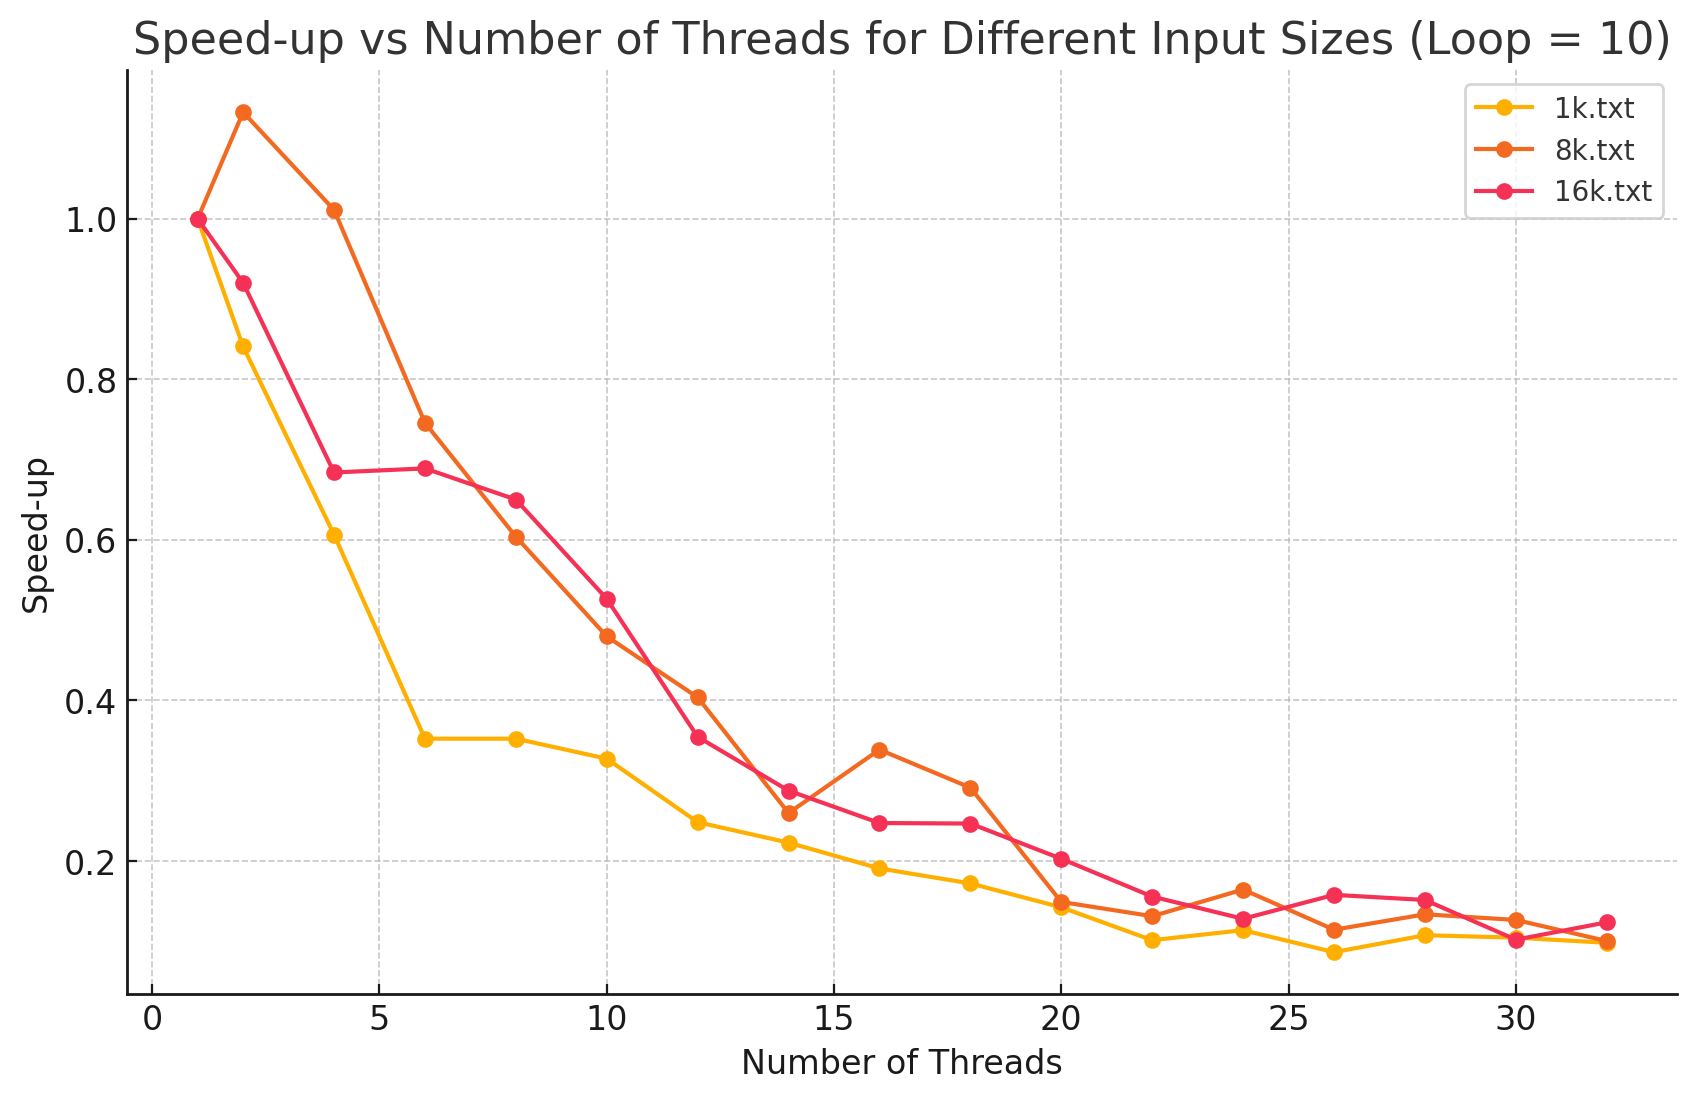
\includegraphics[width=\textwidth]{loop10Sleep.png}
        \caption{Number of Threads VS. Speed-Up}
        \label{fig:ThreadVsSpeedUp1}
    \end{subfigure}
    \hfill  % Horizontal space between figures
    \begin{subfigure}[t]{0.48\textwidth}  % Adjusted width for side-by-side
        \centering
        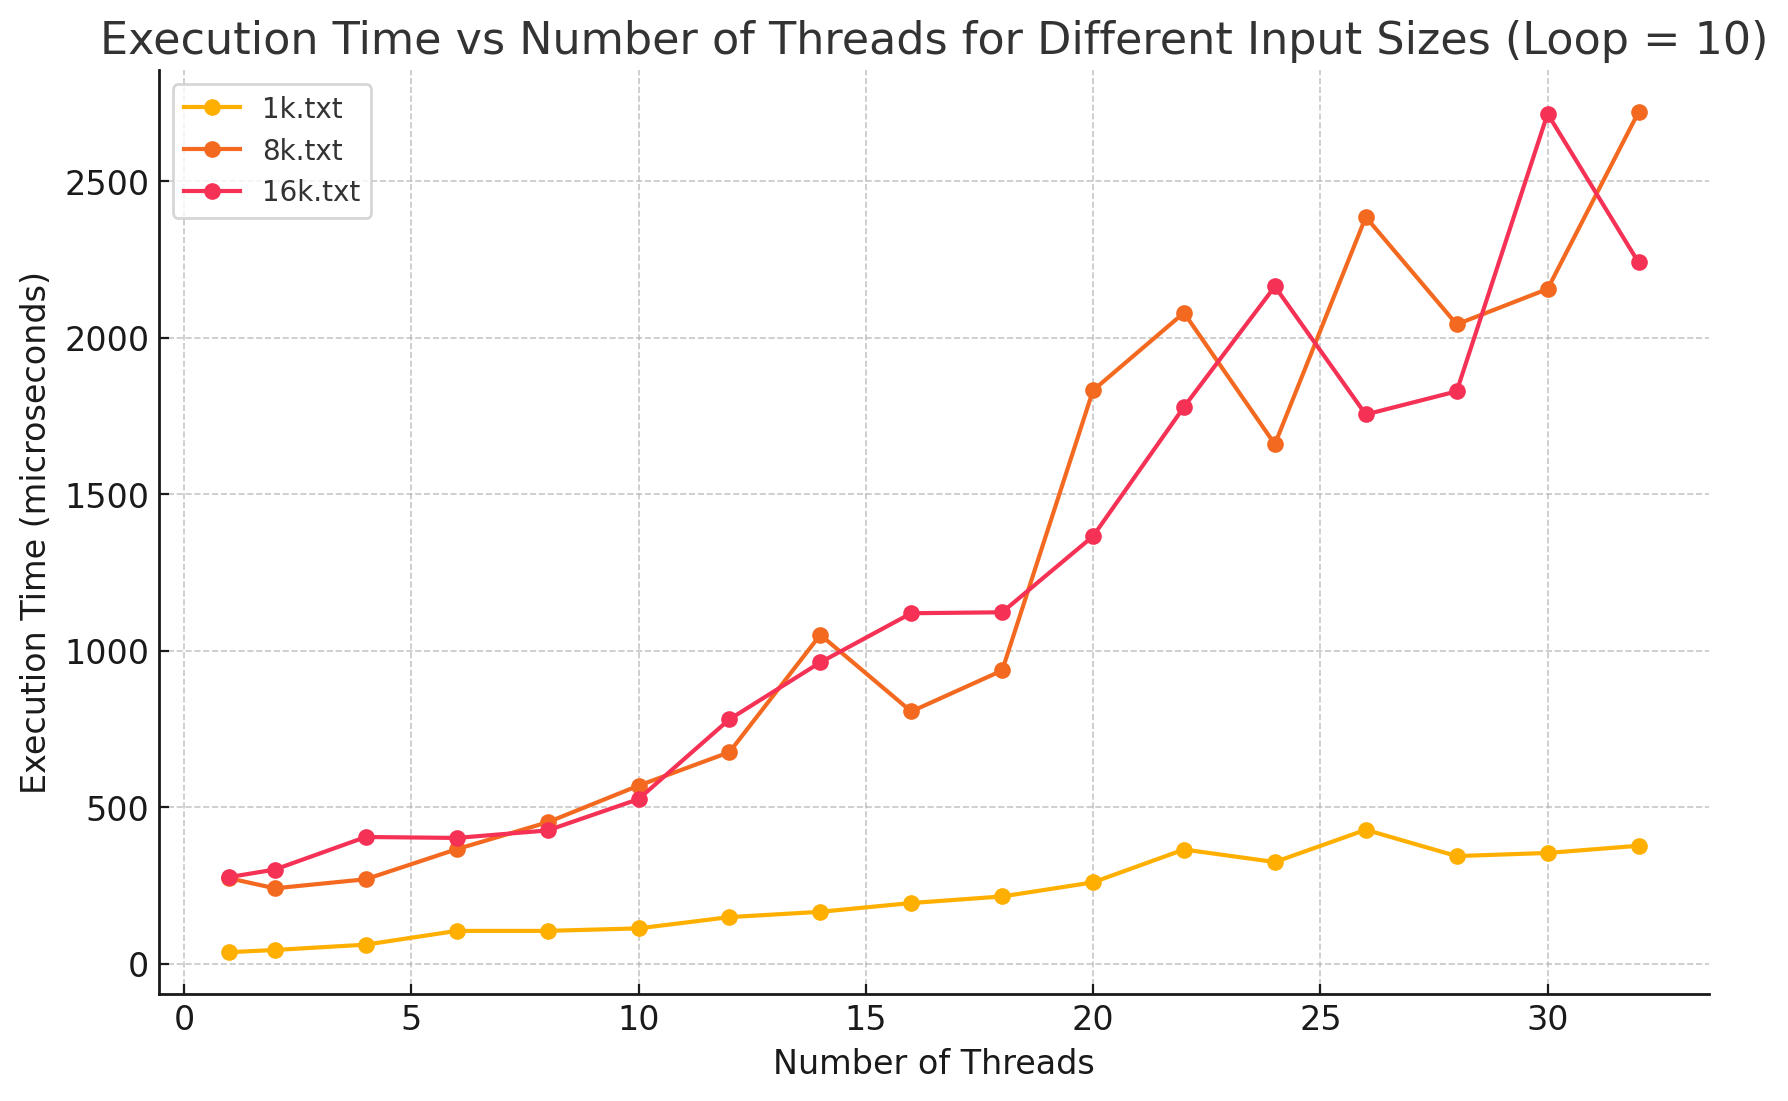
\includegraphics[width=\textwidth]{loop10ExecutionTime.png}
        \caption{Number of Threads VS. Execution Time}
        \label{fig:ThreadVsExecutionTime}
    \end{subfigure}
    \caption{Speed-Up graph and Execution Time graph for loop = 10}
    \label{fig:ThreadVsComparison}
\end{figure}

\hfill  % Horizontal space between figures


\begin{figure}[H]
    \centering
    \begin{subfigure}[t]{0.48\textwidth}  % Adjusted width for side-by-side
        \centering
        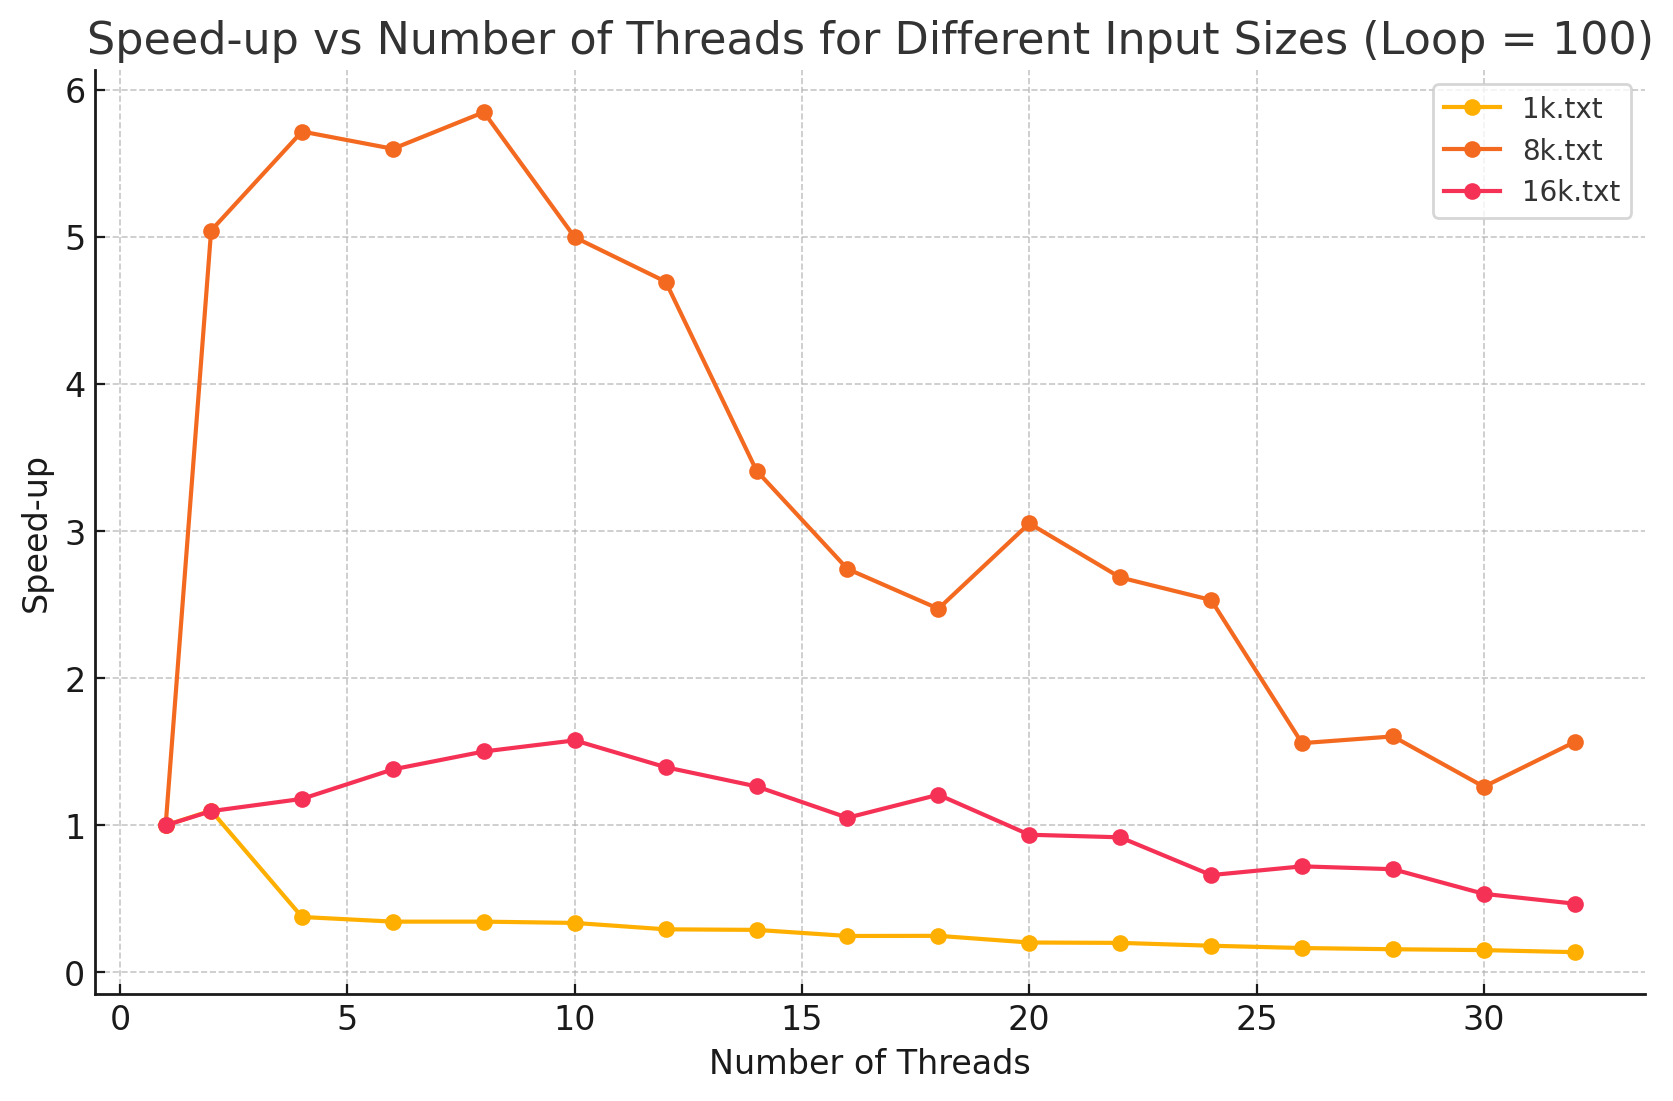
\includegraphics[width=\textwidth]{loop100Sleep.png}
        \caption{Number of Threads VS. Speed-Up}
        \label{fig:ThreadVsSpeedUp1}
    \end{subfigure}
    \hfill  % Horizontal space between figures
    \begin{subfigure}[t]{0.48\textwidth}  % Adjusted width for side-by-side
        \centering
        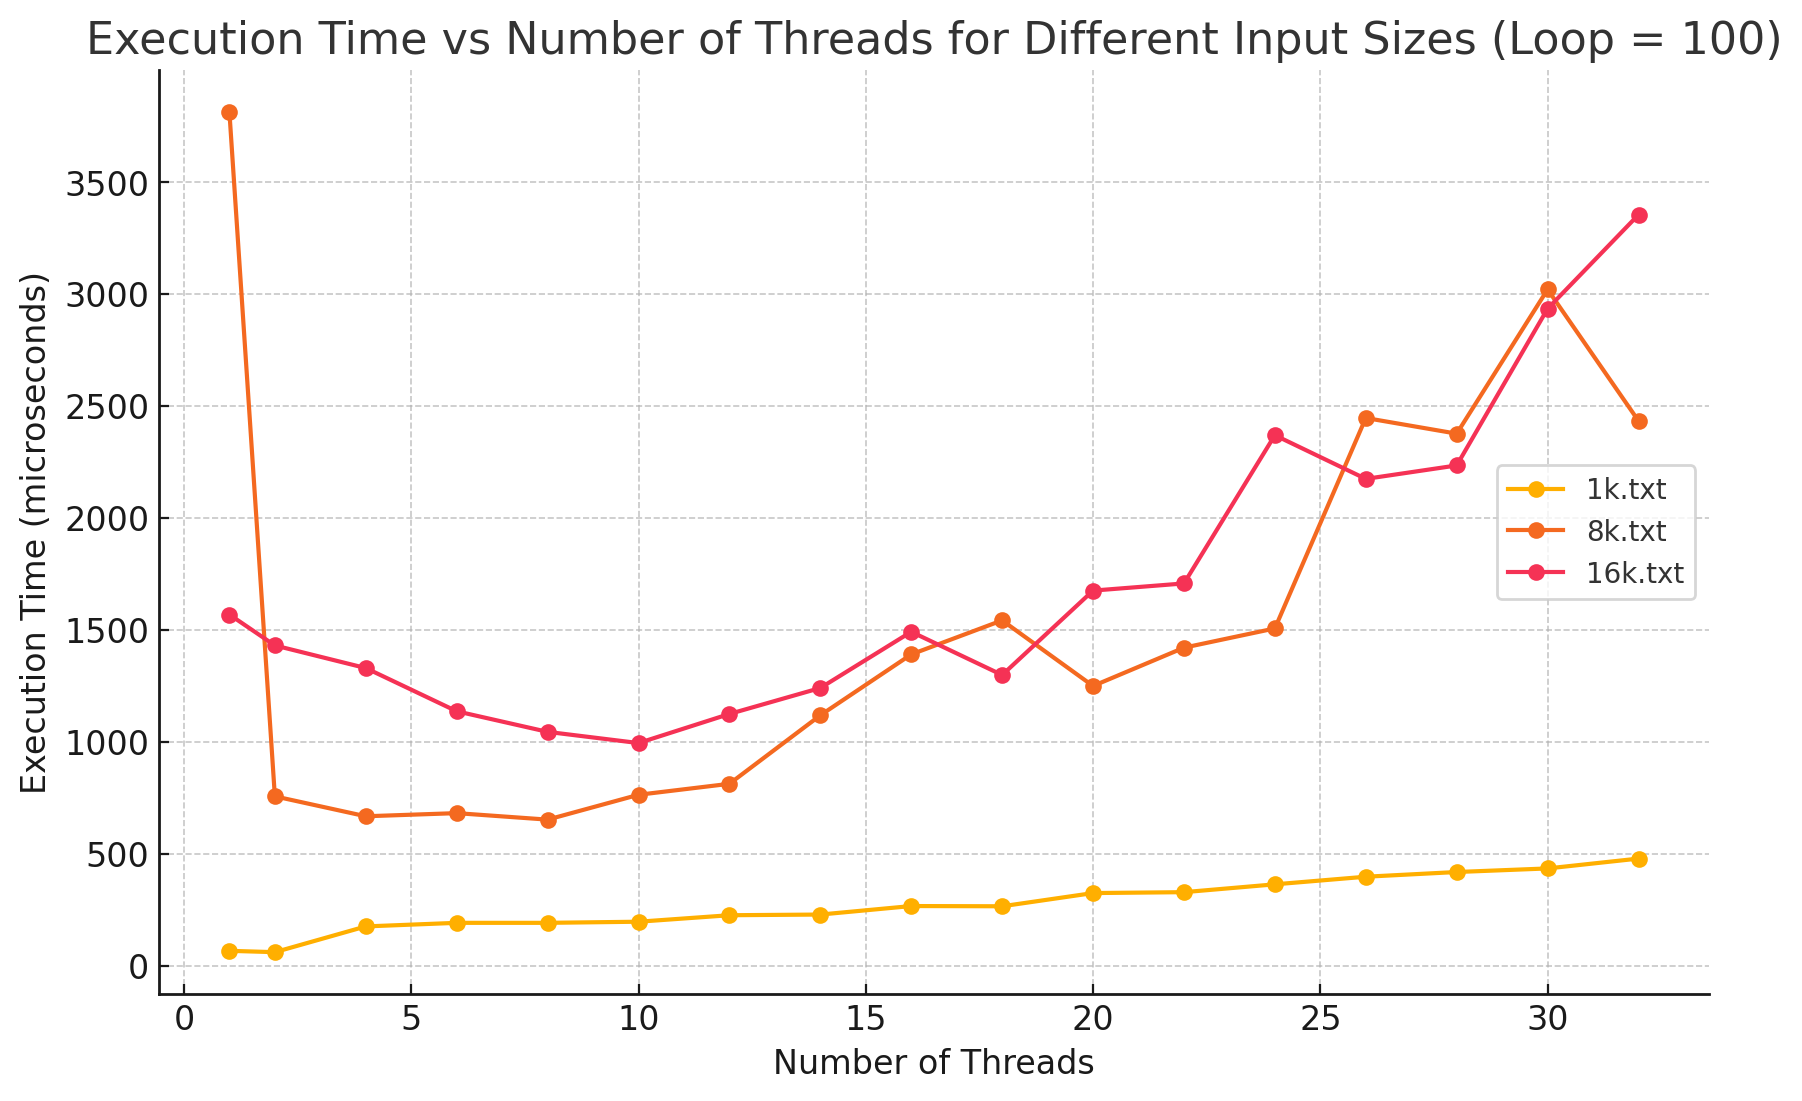
\includegraphics[width=\textwidth]{loop100ExecutionTime.png}
        \caption{Number of Threads VS. Execution Time}
        \label{fig:ThreadVsExecutionTime}
    \end{subfigure}
    \caption{Speed-Up graph and Execution Time graph for loop = 100}
    \label{fig:ThreadVsComparison}
\end{figure}


\hfill  % Horizontal space between figures


\begin{figure}[H]
    \centering
    \begin{subfigure}[t]{0.48\textwidth}  % Adjusted width for side-by-side
        \centering
        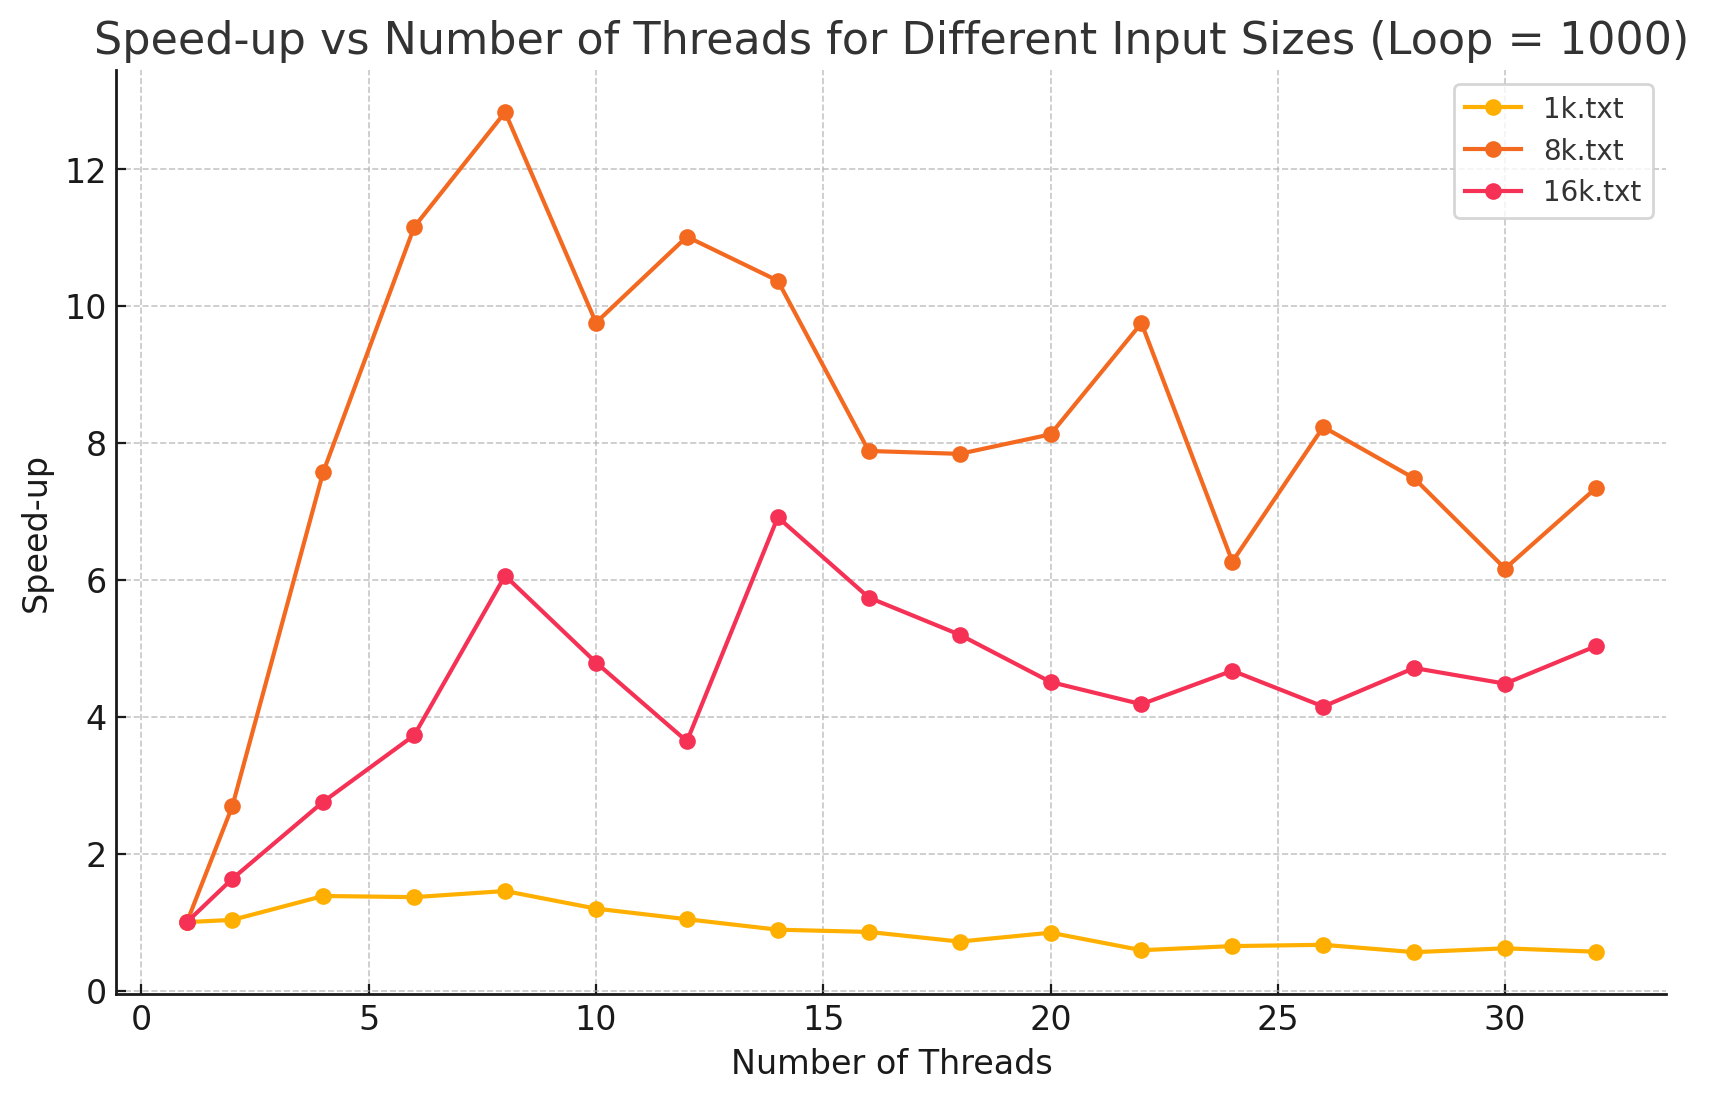
\includegraphics[width=\textwidth]{loop1000Sleep.png}
        \caption{Number of Threads VS. Speed-Up}
        \label{fig:ThreadVsSpeedUp1}
    \end{subfigure}
    \hfill  % Horizontal space between figures
    \begin{subfigure}[t]{0.48\textwidth}  % Adjusted width for side-by-side
        \centering
        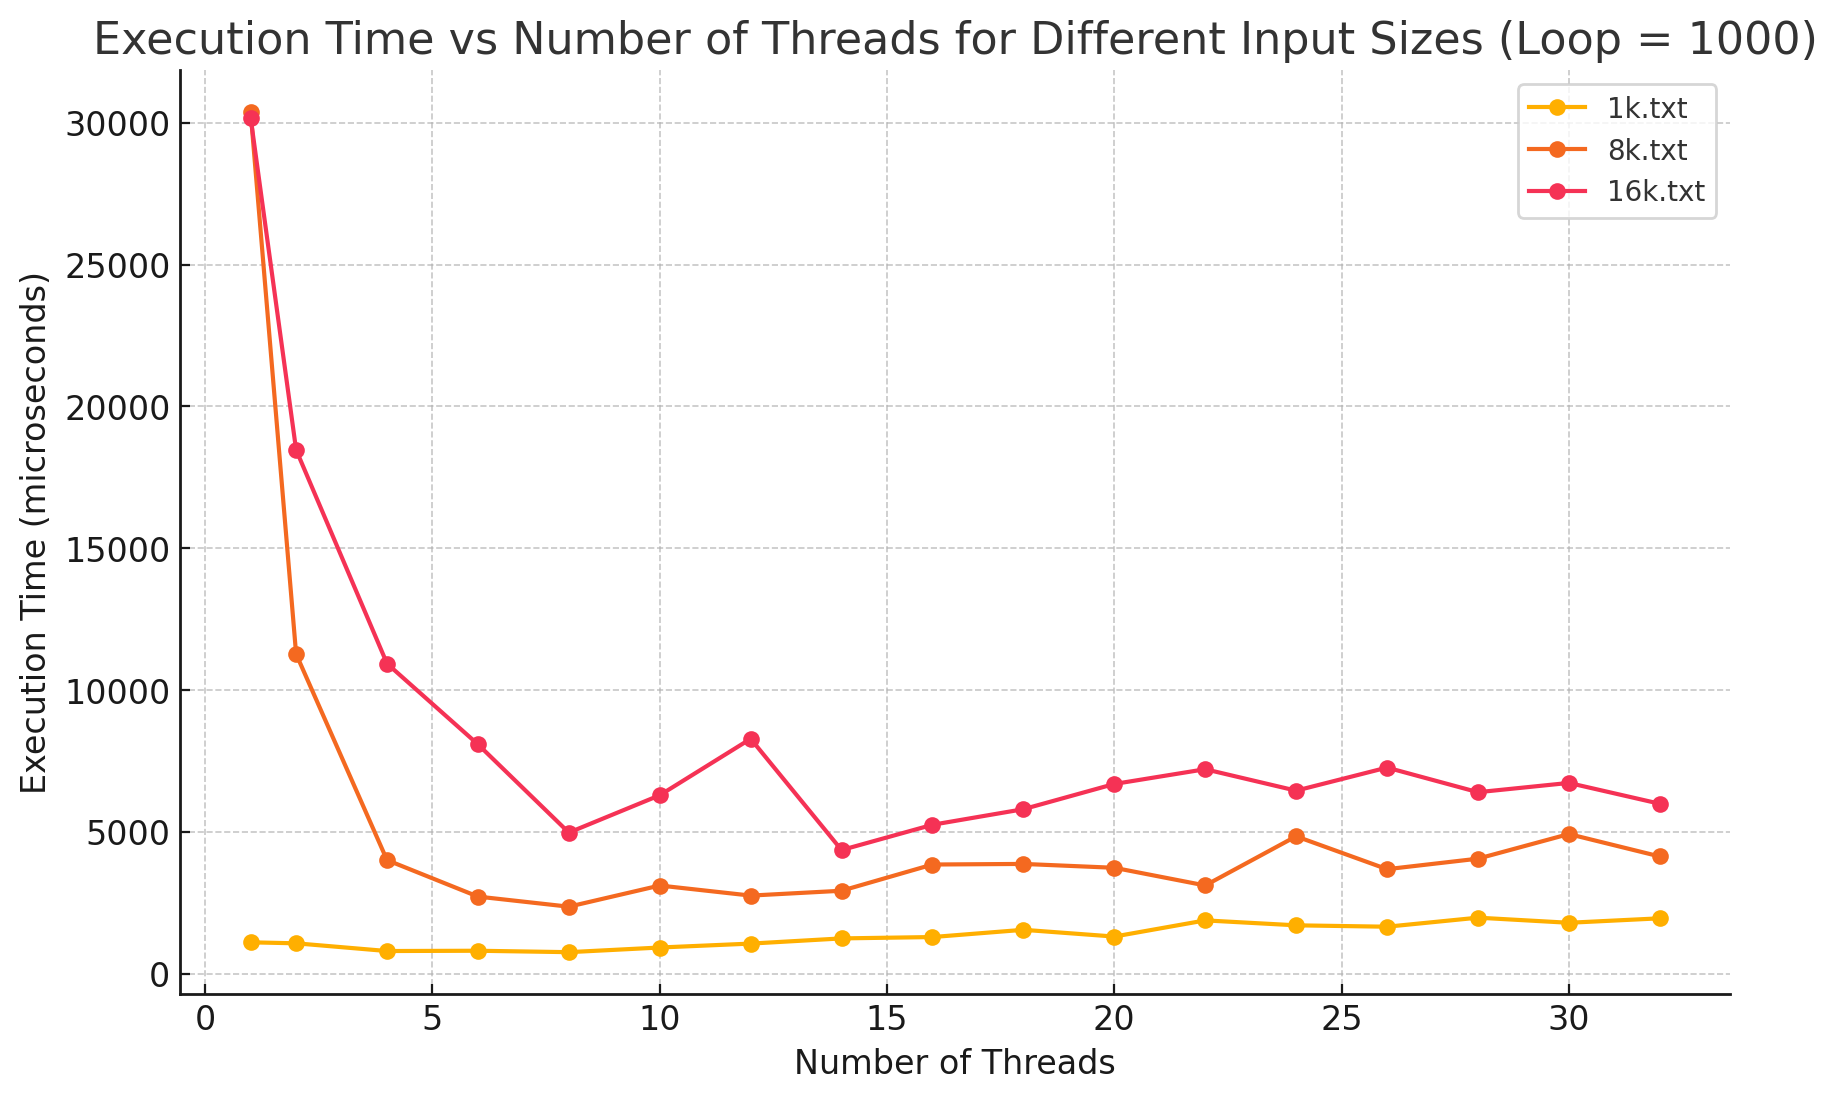
\includegraphics[width=\textwidth]{loop1000ExecutionTime.png}
        \caption{Number of Threads VS. Execution Time}
        \label{fig:ThreadVsExecutionTime}
    \end{subfigure}
    \caption{Speed-Up graph and Execution Time graph for loop = 1000}
    \label{fig:ThreadVsComparison}
\end{figure}


\hfill  % Horizontal space between figures

\begin{figure}[H]
    \centering
    \begin{subfigure}[t]{0.48\textwidth}  % Adjusted width for side-by-side
        \centering
        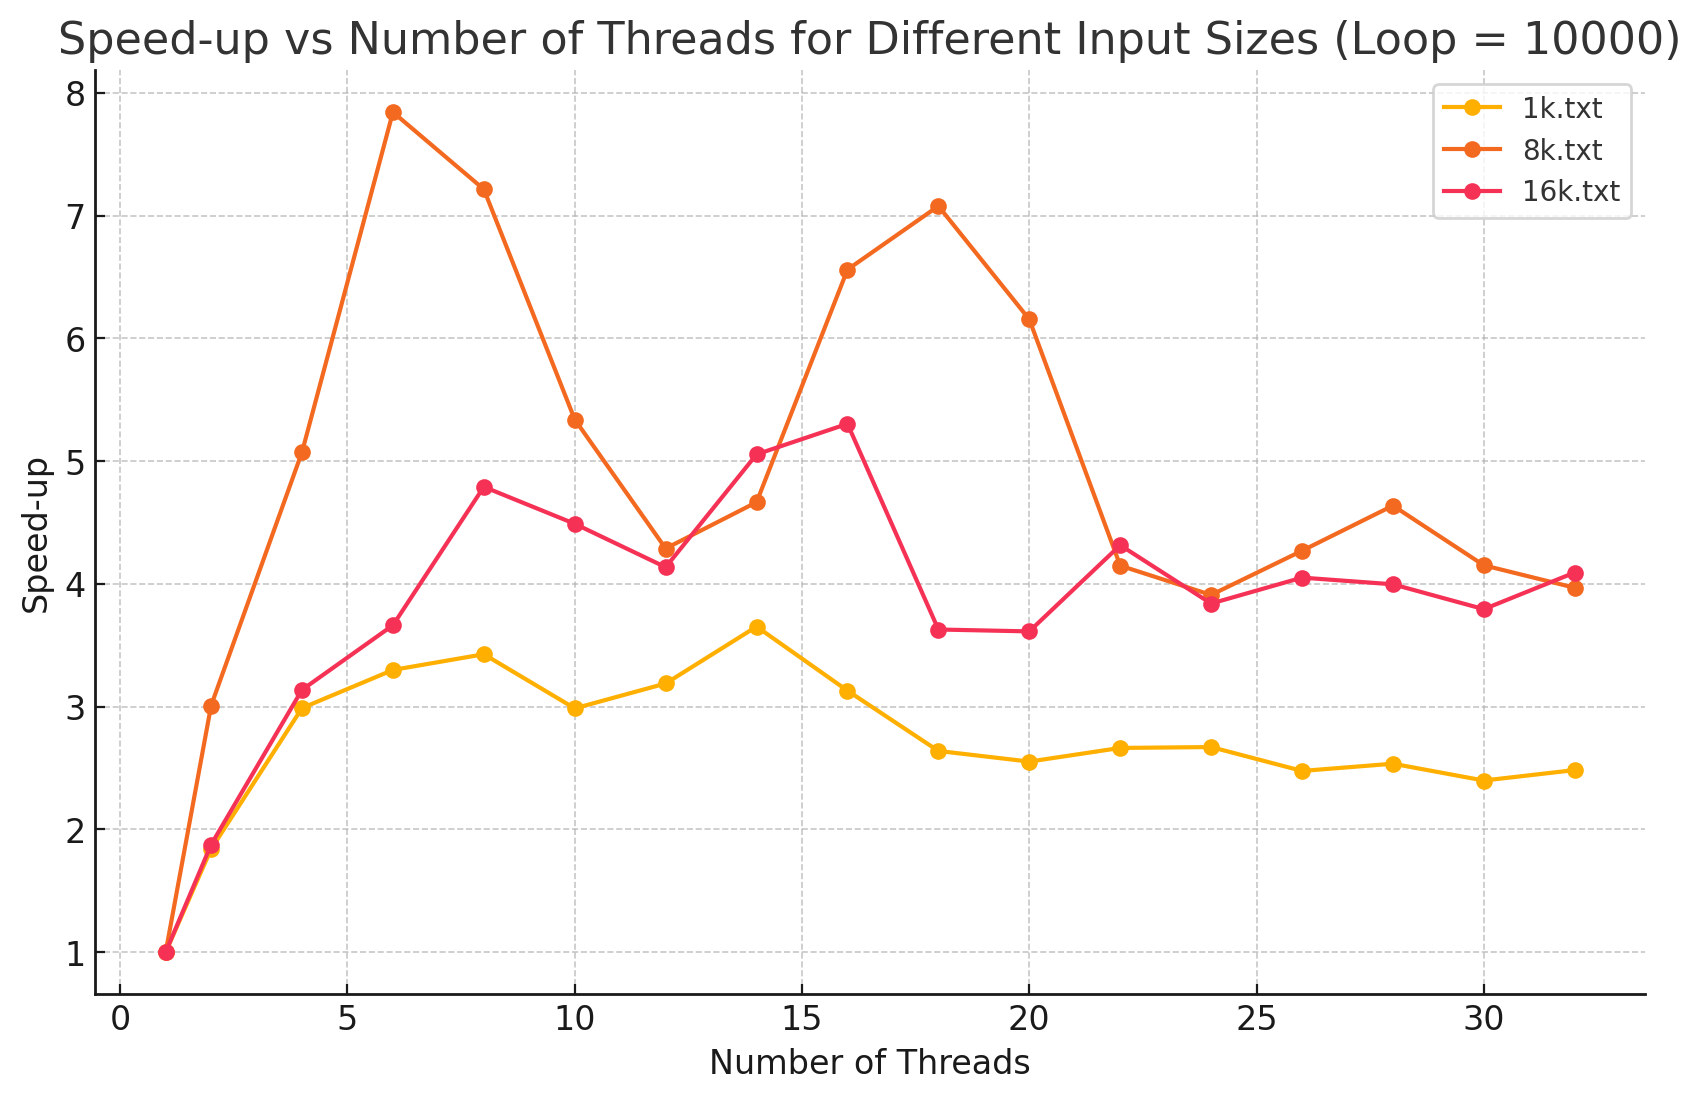
\includegraphics[width=\textwidth]{loop10000Sleep.png}
        \caption{Number of Threads VS. Speed-Up}
        \label{fig:ThreadVsSpeedUp1}
    \end{subfigure}
    \hfill  % Horizontal space between figures
    \begin{subfigure}[t]{0.48\textwidth}  % Adjusted width for side-by-side
        \centering
        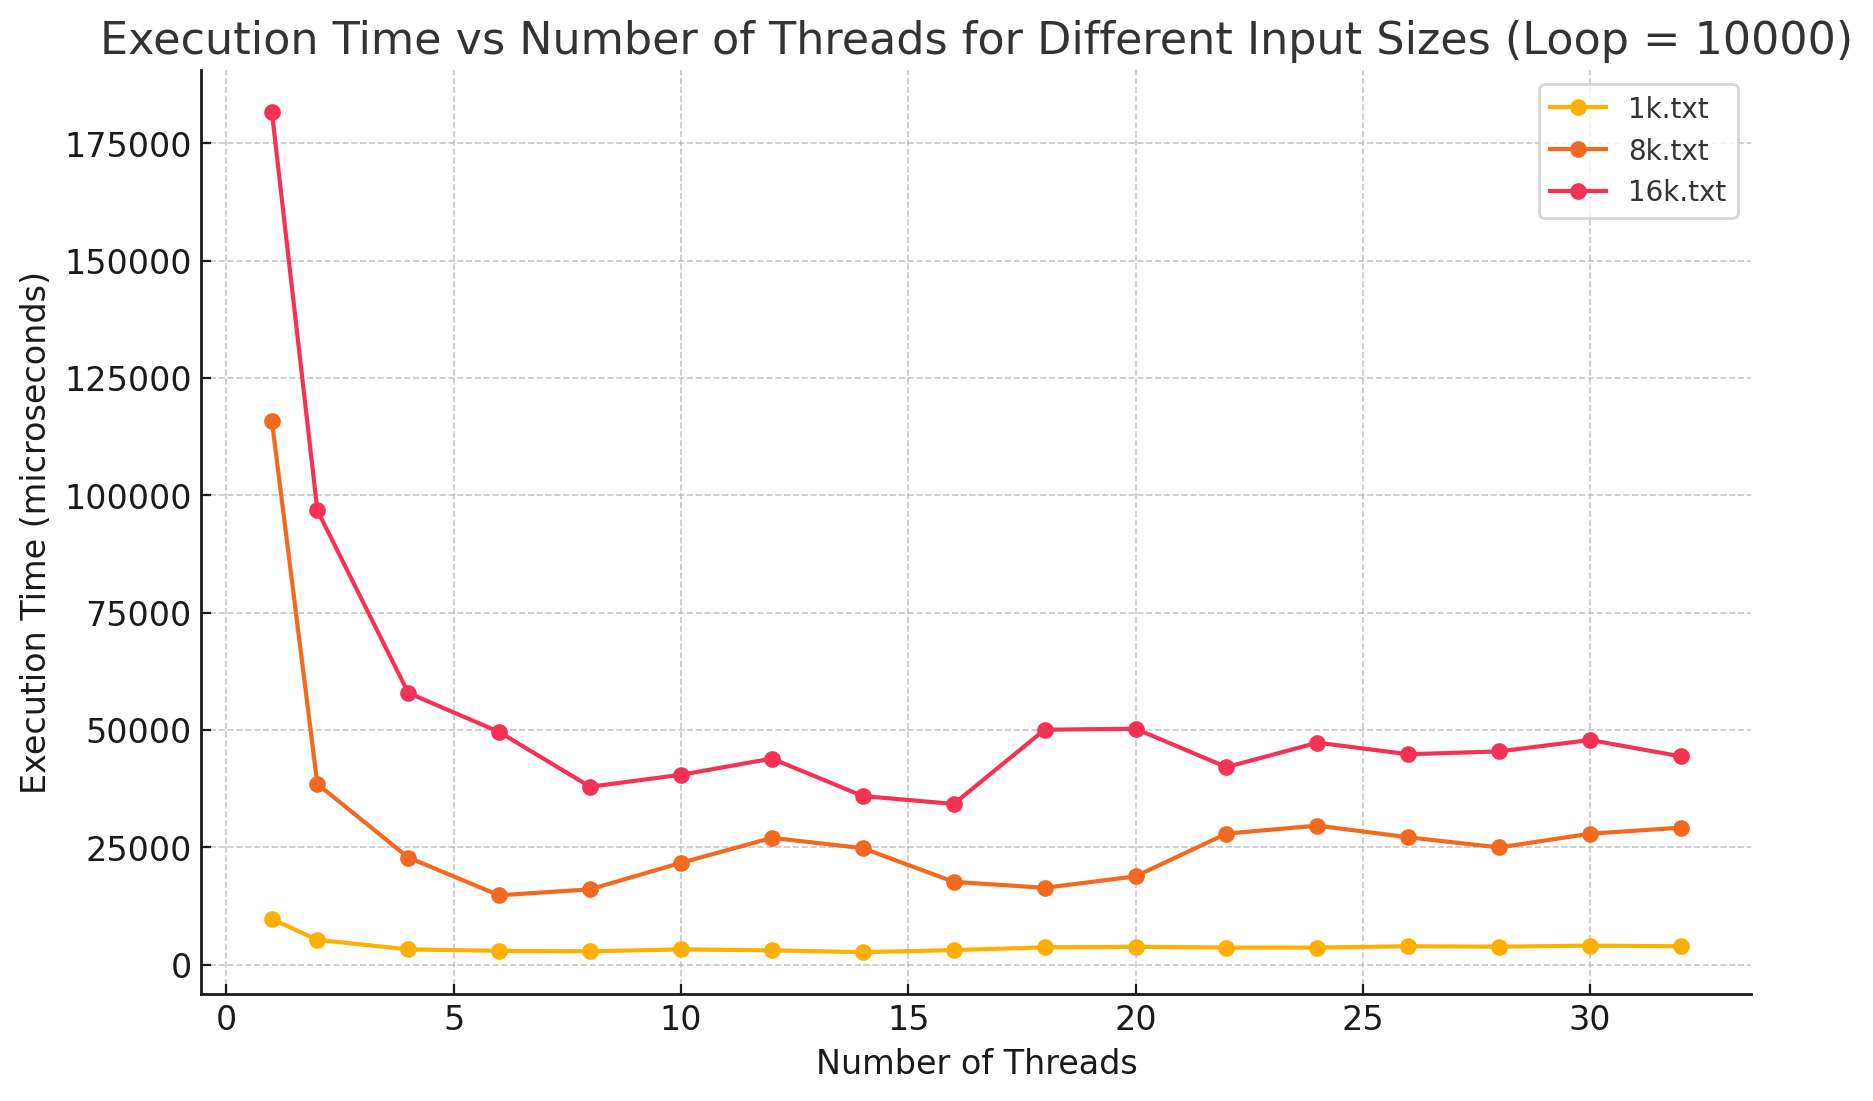
\includegraphics[width=\textwidth]{loop10000ExecutionTime.png}
        \caption{Number of Threads VS. Execution Time}
        \label{fig:ThreadVsExecutionTime}
    \end{subfigure}
    \caption{Speed-Up graph and Execution Time graph for loop = 10000}
    \label{fig:ThreadVsComparison}
\end{figure}

\hfill  % Horizontal space between figures


\begin{figure}[H]
    \centering
    \begin{subfigure}[t]{0.48\textwidth}  % Adjusted width for side-by-side
        \centering
        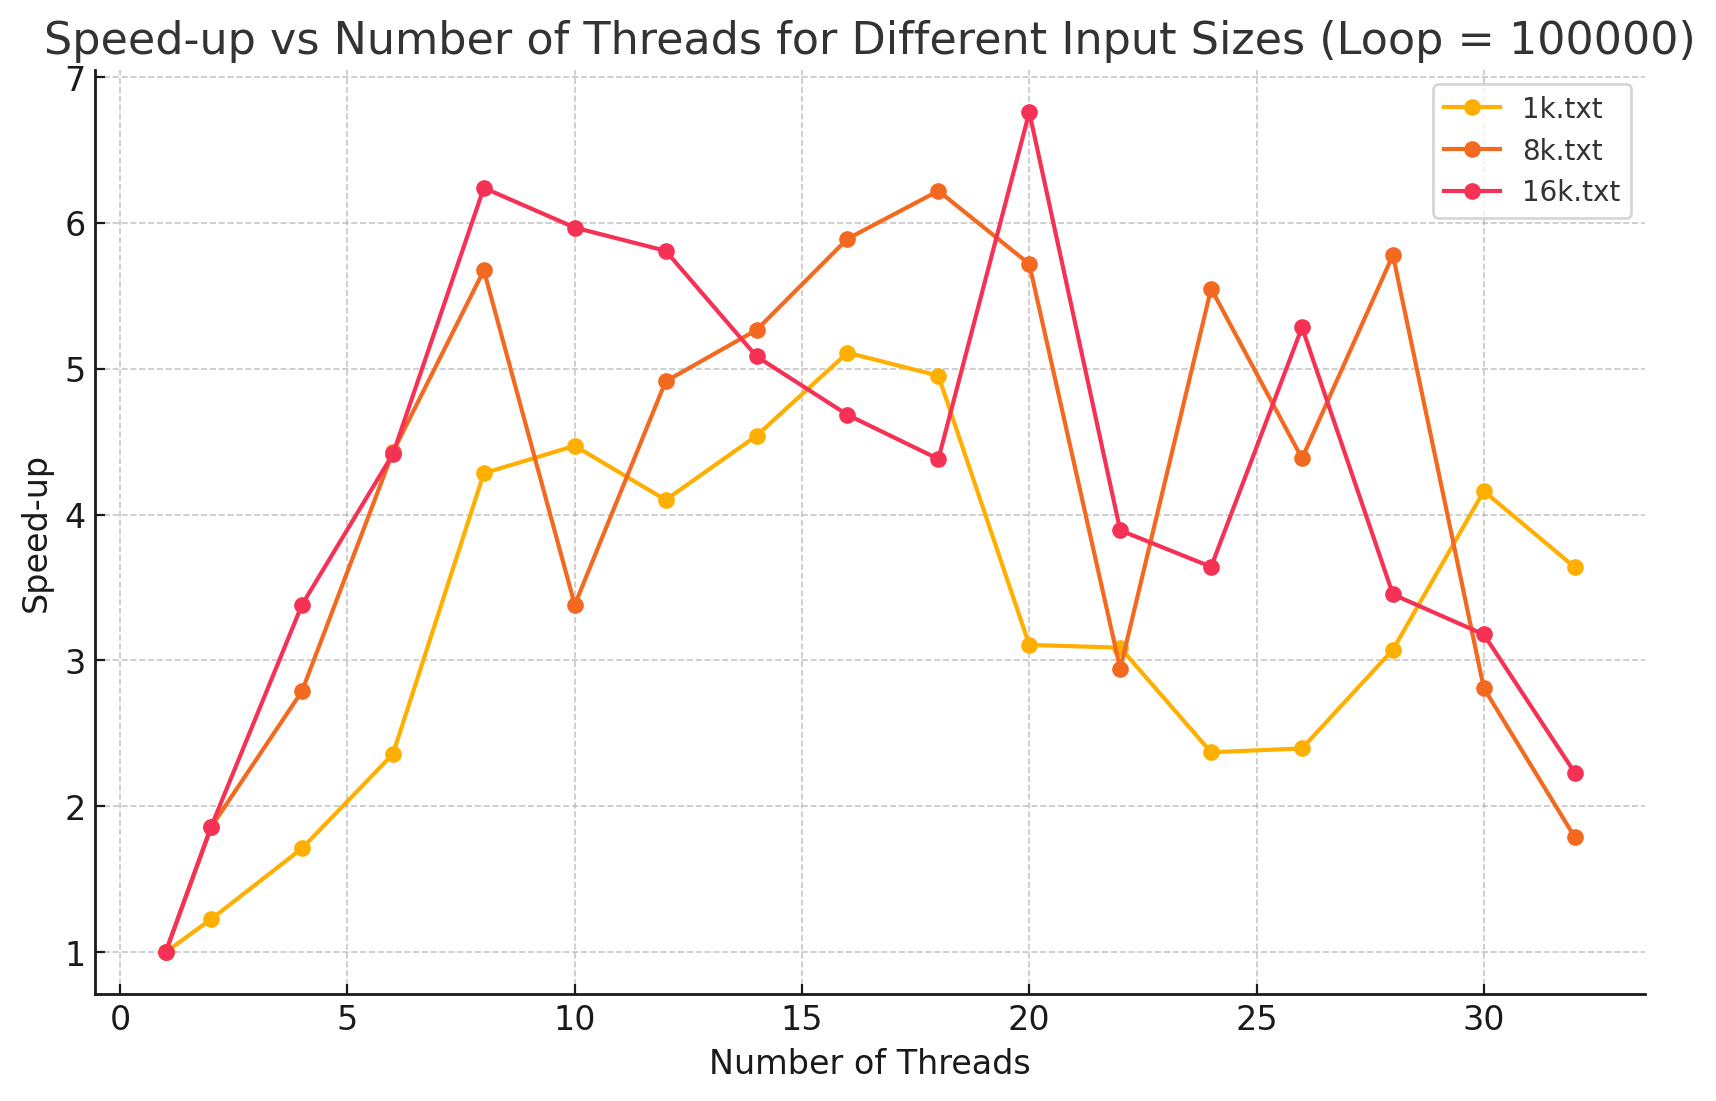
\includegraphics[width=\textwidth]{loop100000Sleep.png}
        \caption{Number of Threads VS. Speed-Up}
        \label{fig:ThreadVsSpeedUp1}
    \end{subfigure}
    \hfill  % Horizontal space between figures
    \begin{subfigure}[t]{0.48\textwidth}  % Adjusted width for side-by-side
        \centering
        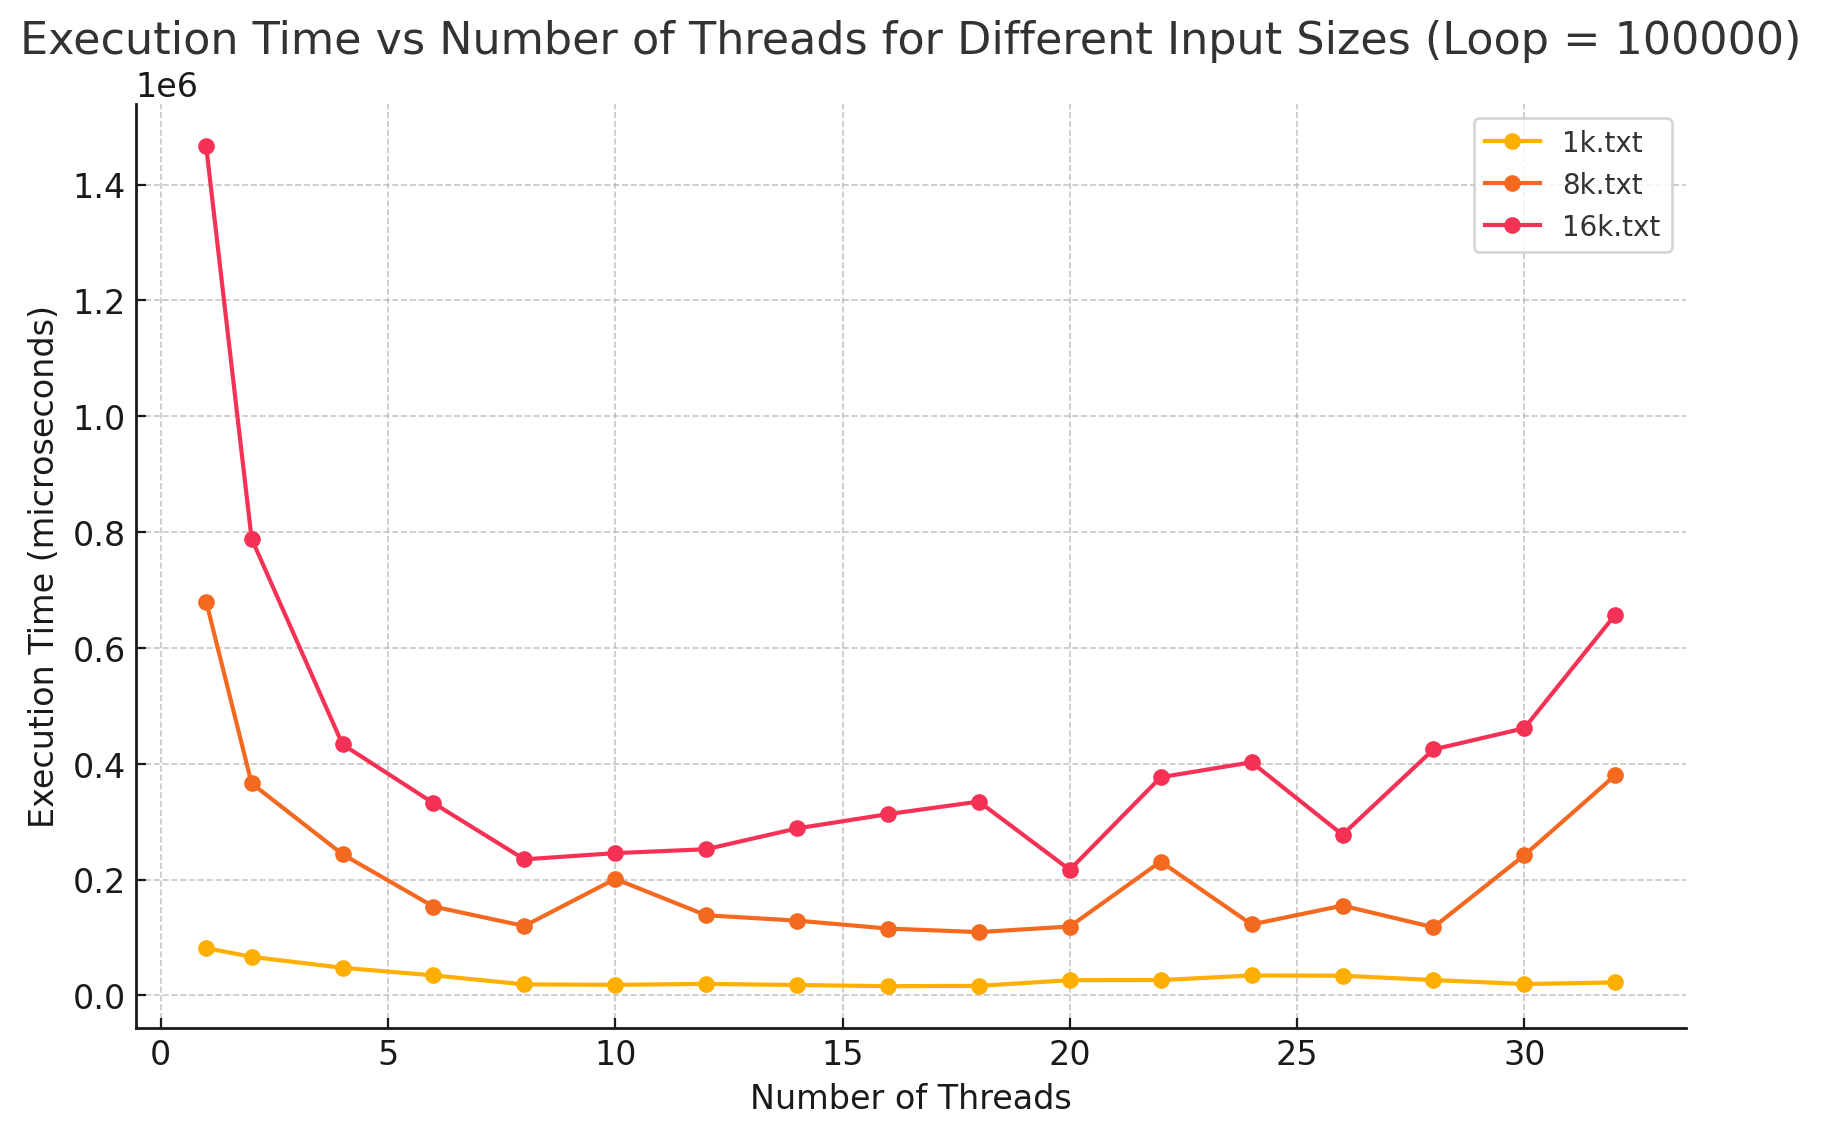
\includegraphics[width=\textwidth]{loop100000ExecutionTime.png}
        \caption{Number of Threads VS. Execution Time}
        \label{fig:ThreadVsExecutionTime}
    \end{subfigure}
    \caption{Speed-Up graph and Execution Time graph for loop = 100000}
    \label{fig:ThreadVsComparison}
\end{figure}

\hfill  % Horizontal space between figures

\begin{figure}[H]
    \centering
    \begin{subfigure}[t]{0.48\textwidth}  % Adjusted width for side-by-side
        \centering
        \includegraphics[width=\textwidth]{loop1000000Sleep.png}
        \caption{Number of Threads VS. Speed-Up}
        \label{fig:ThreadVsSpeedUp1}
    \end{subfigure}
    \hfill  % Horizontal space between figures
    \begin{subfigure}[t]{0.48\textwidth}  % Adjusted width for side-by-side
        \centering
        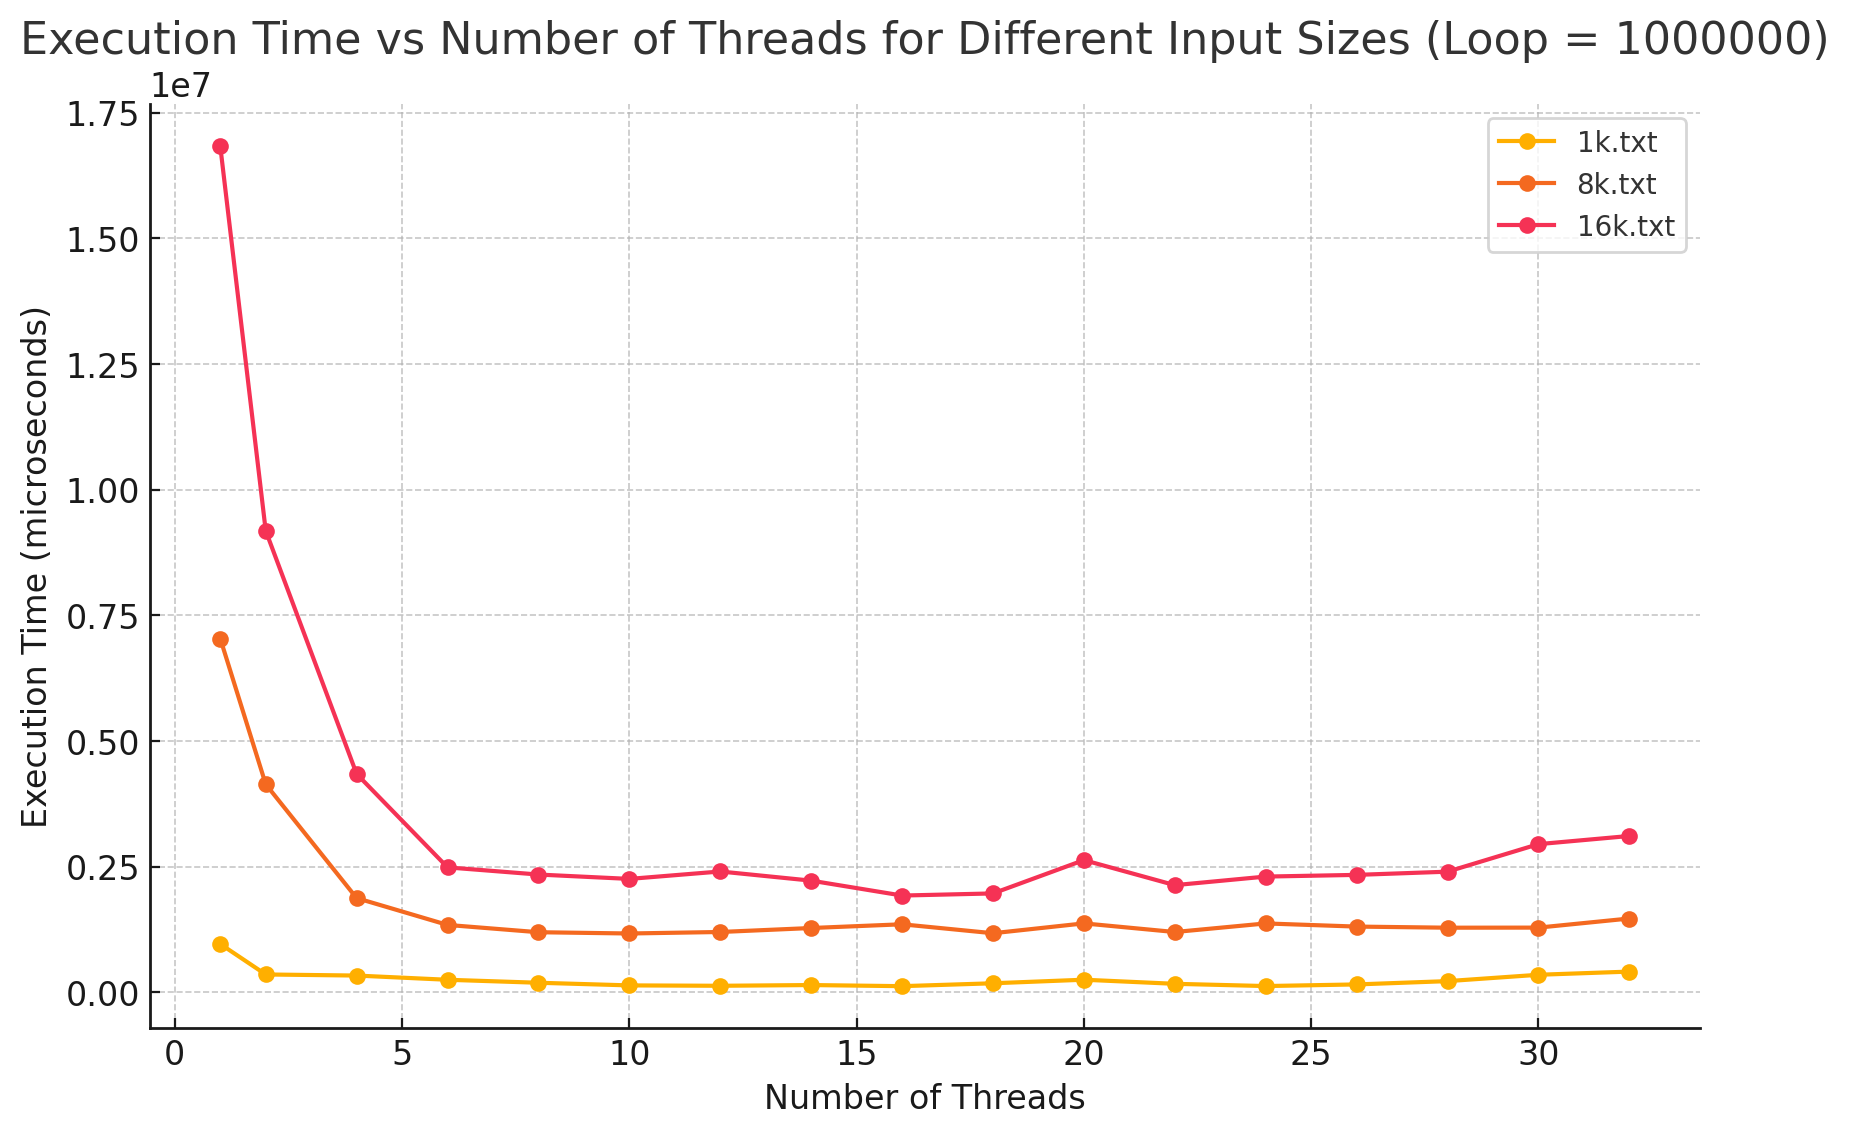
\includegraphics[width=\textwidth]{loop1000000ExecutionTime.png}
        \caption{Number of Threads VS. Execution Time}
        \label{fig:ThreadVsExecutionTime}
    \end{subfigure}
    \caption{Speed-Up graph and Execution Time graph for loop = 1000000}
    \label{fig:ThreadVsComparison}
\end{figure}



\subsection{Speedup analysis with yield (simple counter based spin-barrier) }

\begin{figure}[H]
    \centering
    \begin{subfigure}[t]{0.48\textwidth}  % Adjusted width for side-by-side
        \centering
        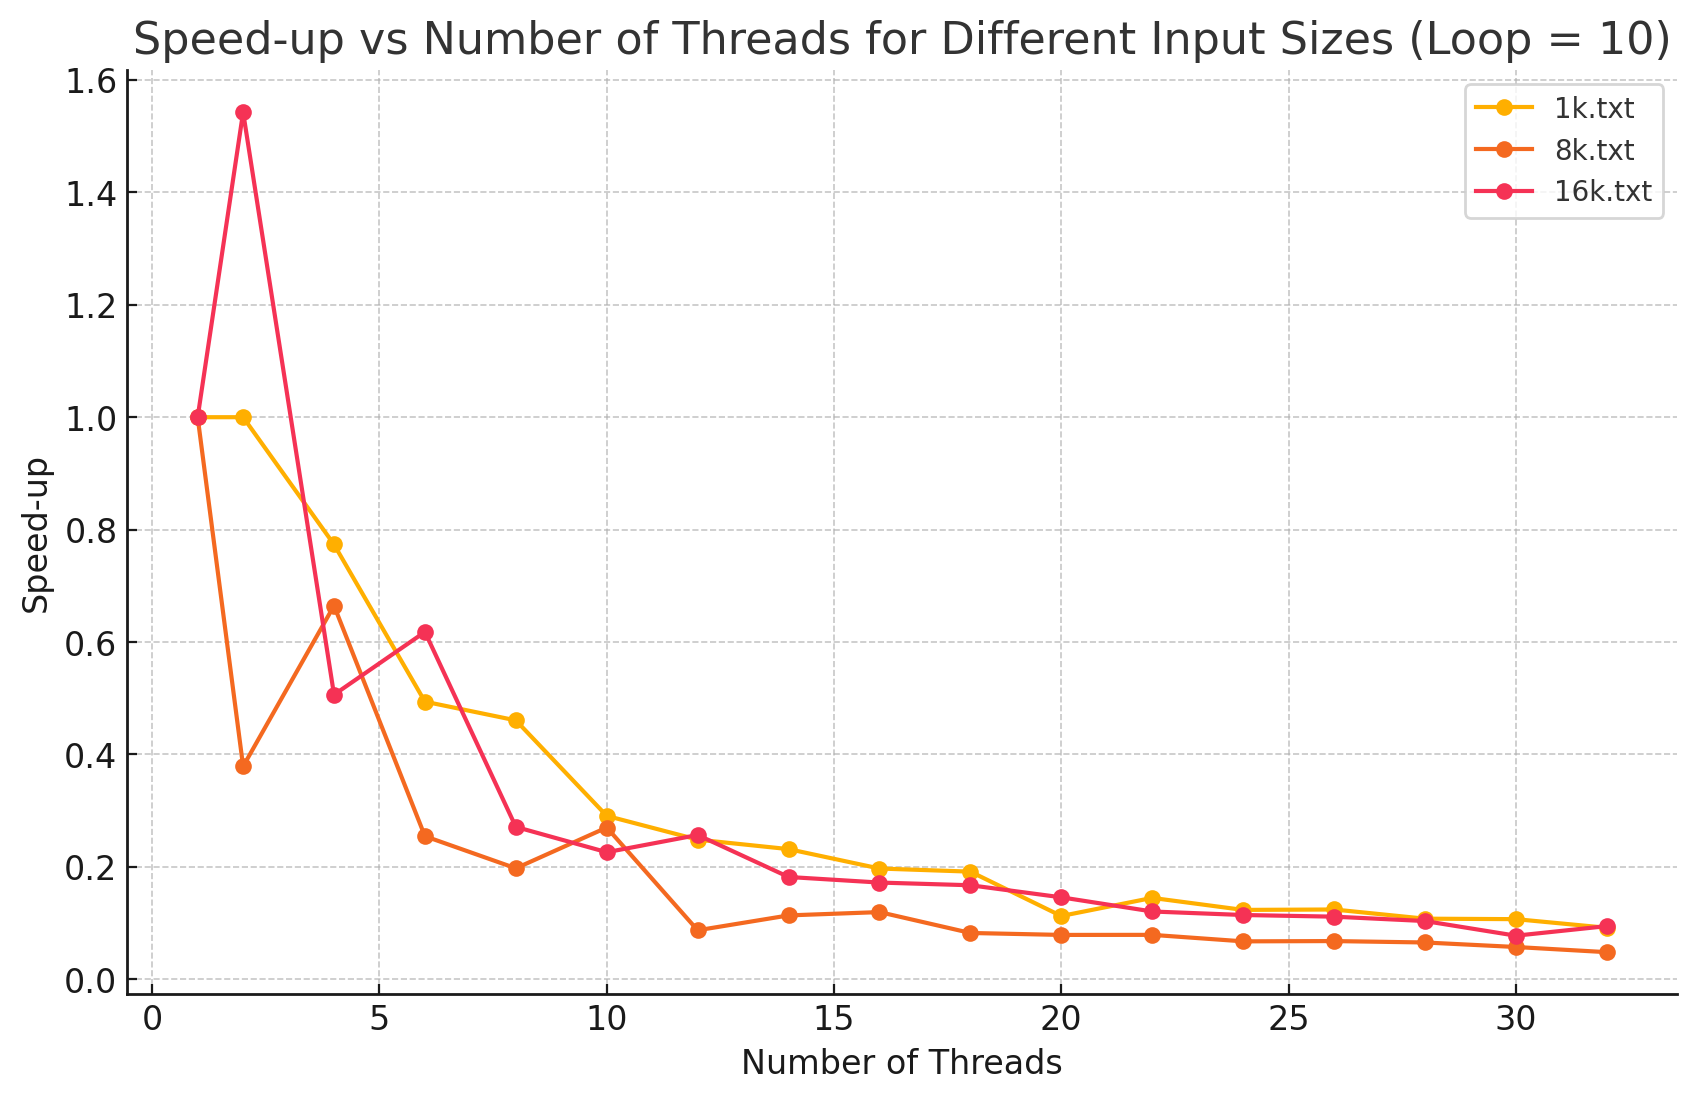
\includegraphics[width=\textwidth]{loop10Yield.png}
        \caption{Number of Threads VS. Speed-Up}
        \label{fig:ThreadVsSpeedUp1}
    \end{subfigure}
    \hfill  % Horizontal space between figures
    \begin{subfigure}[t]{0.48\textwidth}  % Adjusted width for side-by-side
        \centering
        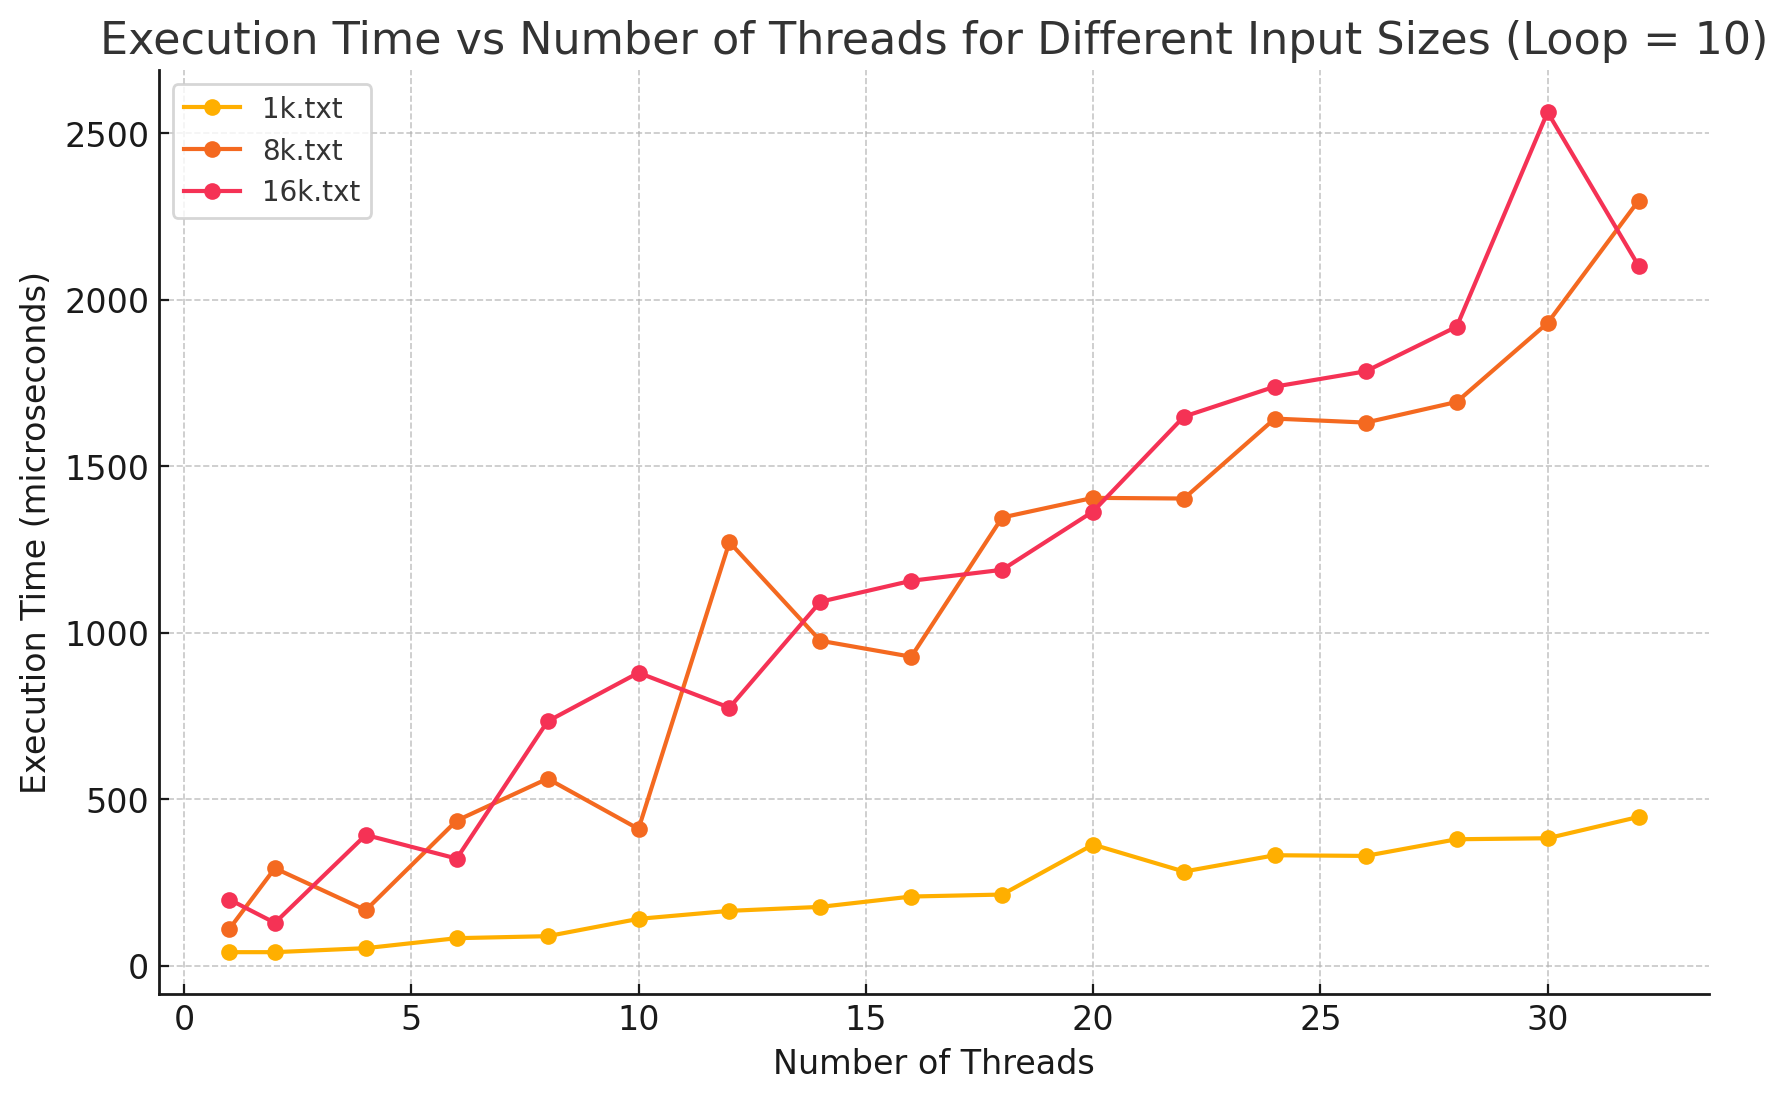
\includegraphics[width=\textwidth]{loop10YieldExecutionTime.png}
        \caption{Number of Threads VS. Execution Time}
        \label{fig:ThreadVsExecutionTime}
    \end{subfigure}
    \caption{Speed-Up graph and Execution Time graph for loop = 10}
    \label{fig:ThreadVsComparison}
\end{figure}

\hfill  % Horizontal space between figures

\begin{figure}[H]
    \centering
    \begin{subfigure}[t]{0.48\textwidth}  % Adjusted width for side-by-side
        \centering
        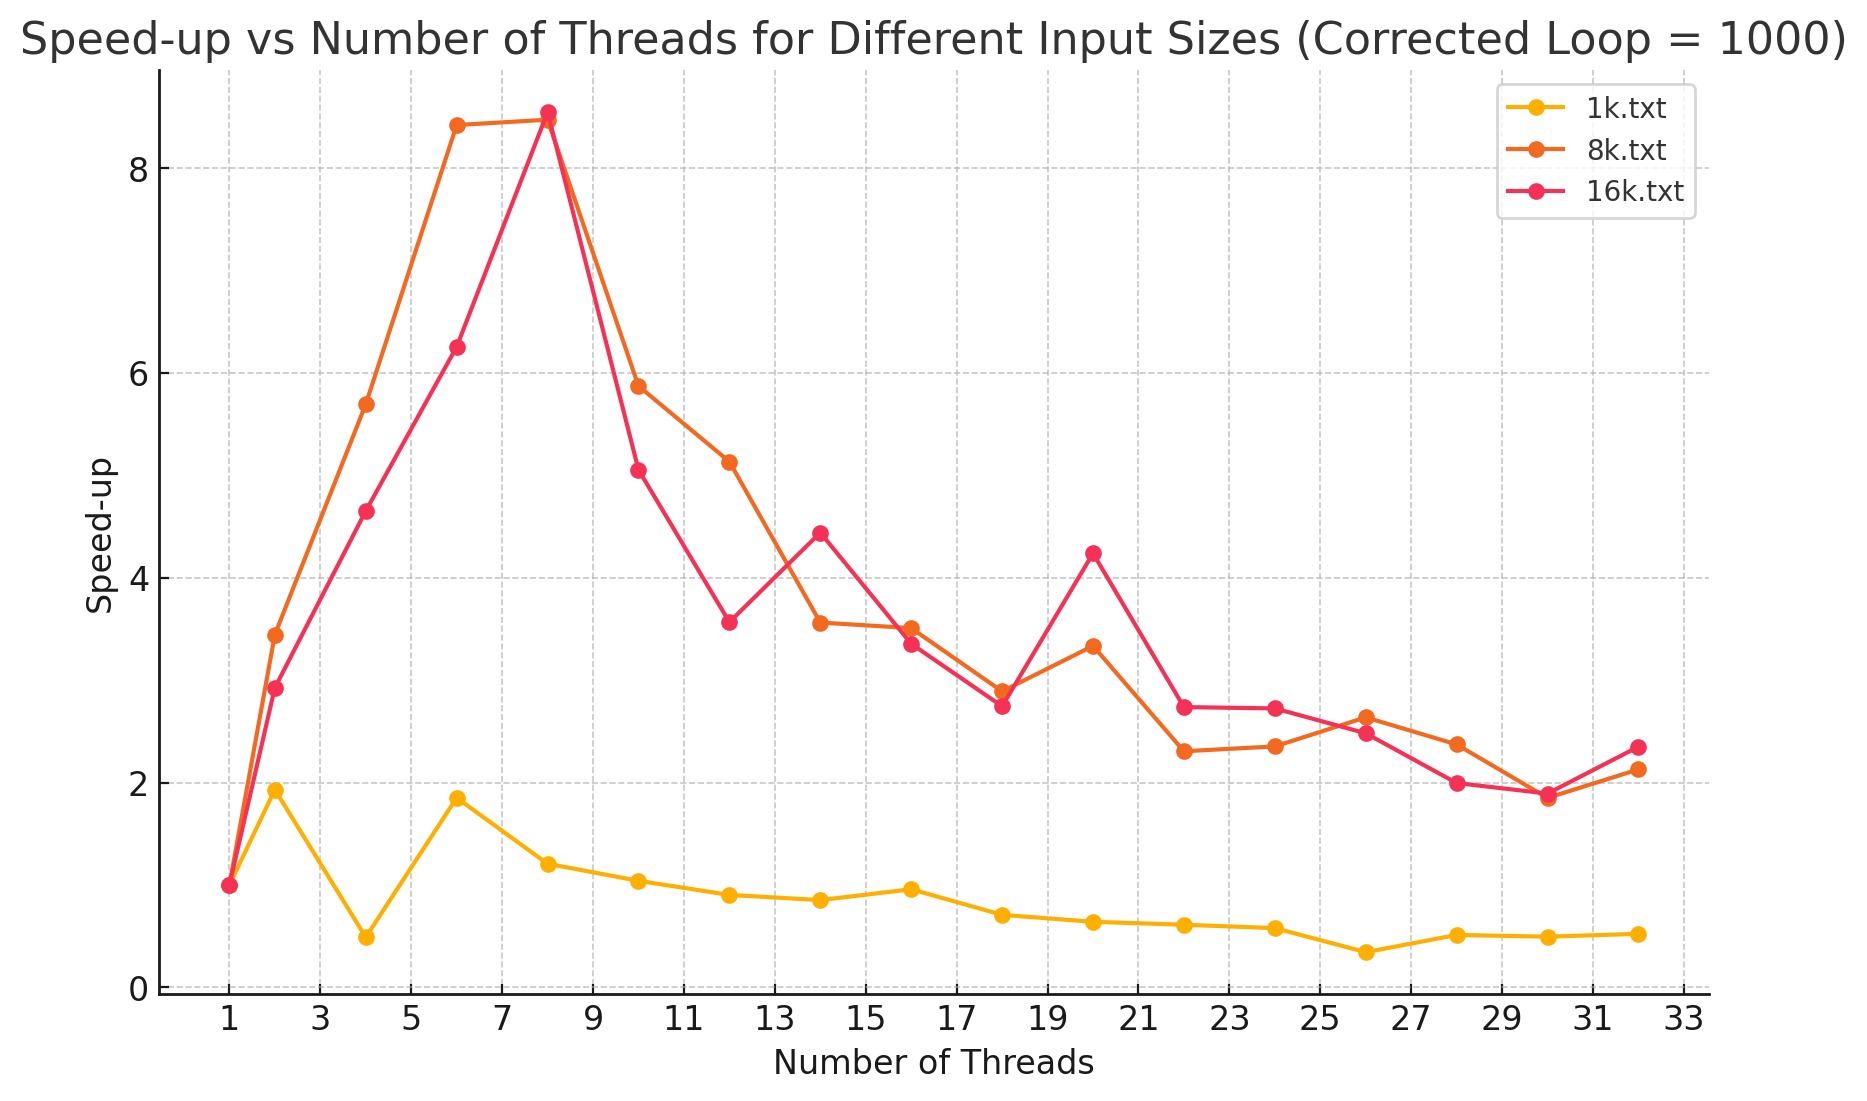
\includegraphics[width=\textwidth]{loop1000Yield.png}
        \caption{Number of Threads VS. Speed-Up}
        \label{fig:ThreadVsSpeedUp1}
    \end{subfigure}
    \hfill  % Horizontal space between figures
    \begin{subfigure}[t]{0.48\textwidth}  % Adjusted width for side-by-side
        \centering
        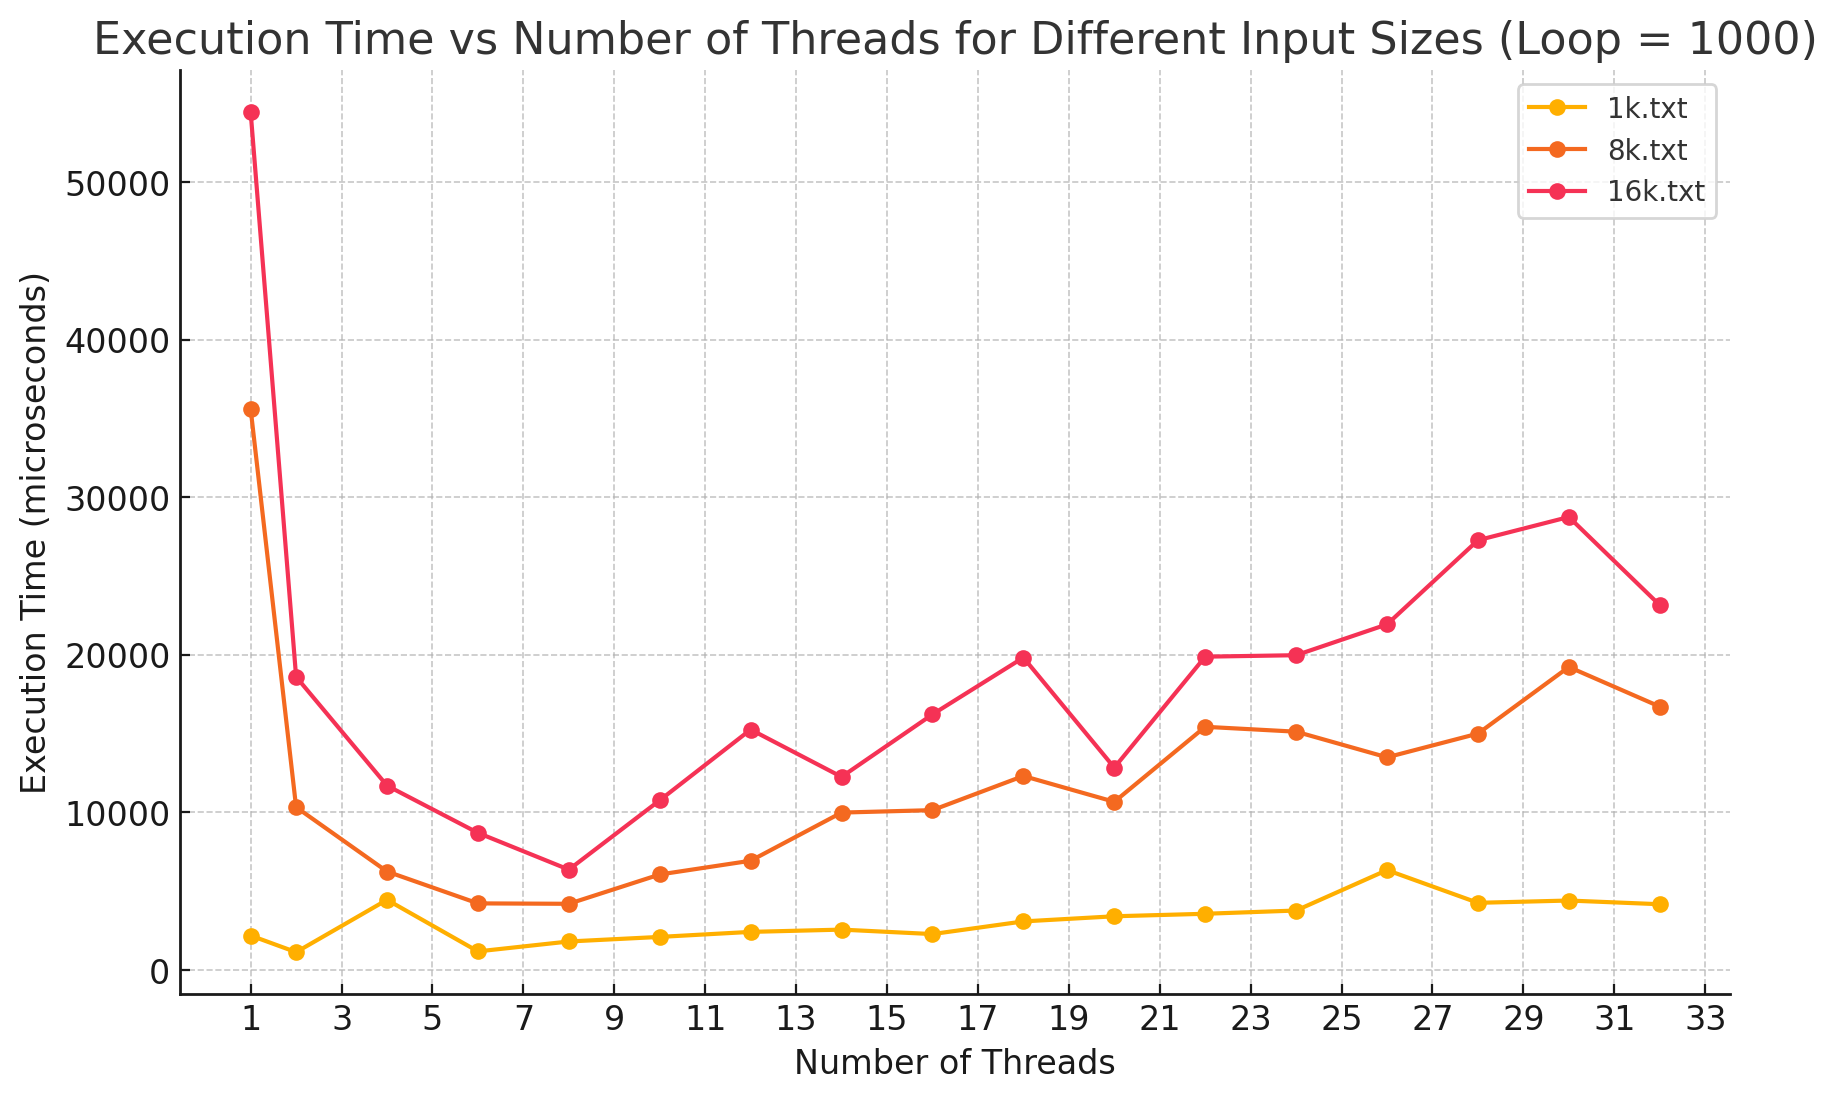
\includegraphics[width=\textwidth]{loop1000YieldExecutionTime.png}
        \caption{Number of Threads VS. Execution Time}
        \label{fig:ThreadVsExecutionTime}
    \end{subfigure}
    \caption{Speed-Up graph and Execution Time graph for loop = 1000}
    \label{fig:ThreadVsComparison}
\end{figure}
\hfill  % Horizontal space between figures


\begin{figure}[H]
    \centering
    \begin{subfigure}[t]{0.48\textwidth}  % Adjusted width for side-by-side
        \centering
        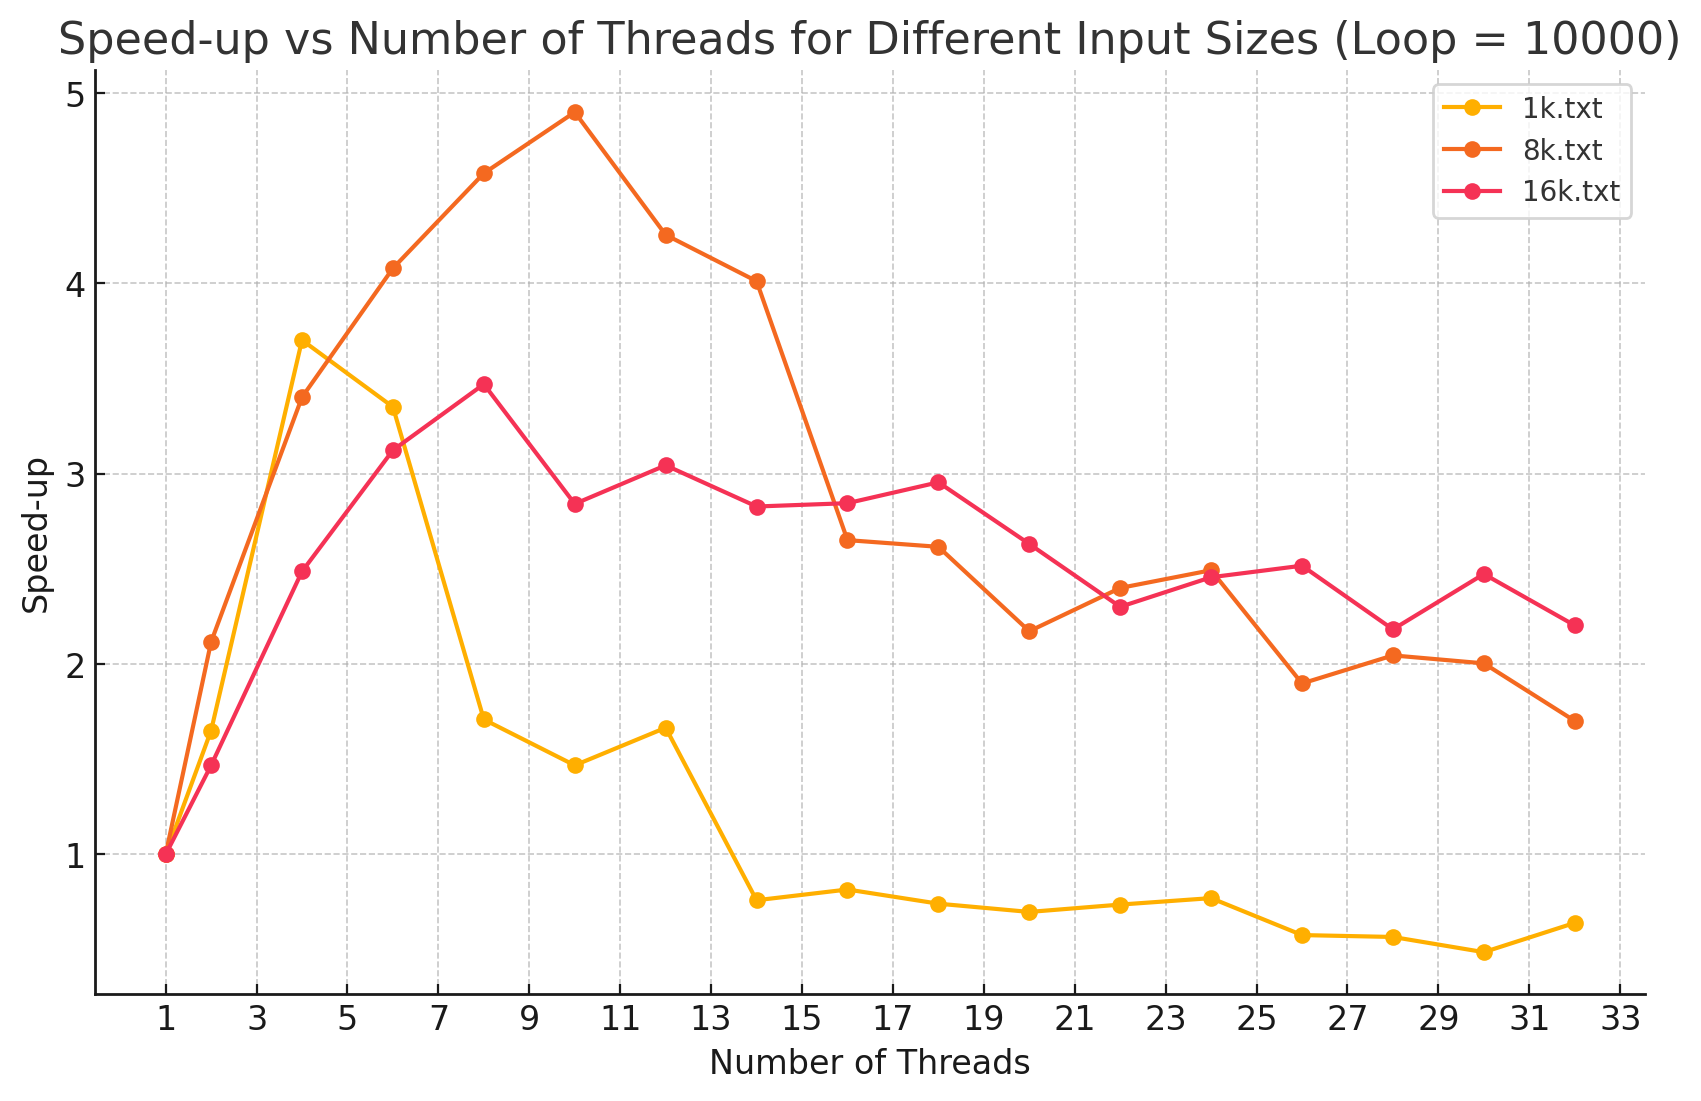
\includegraphics[width=\textwidth]{loop10000Yield.png}
        \caption{Number of Threads VS. Speed-Up}
        \label{fig:ThreadVsSpeedUp1}
    \end{subfigure}
    \hfill  % Horizontal space between figures
    \begin{subfigure}[t]{0.48\textwidth}  % Adjusted width for side-by-side
        \centering
        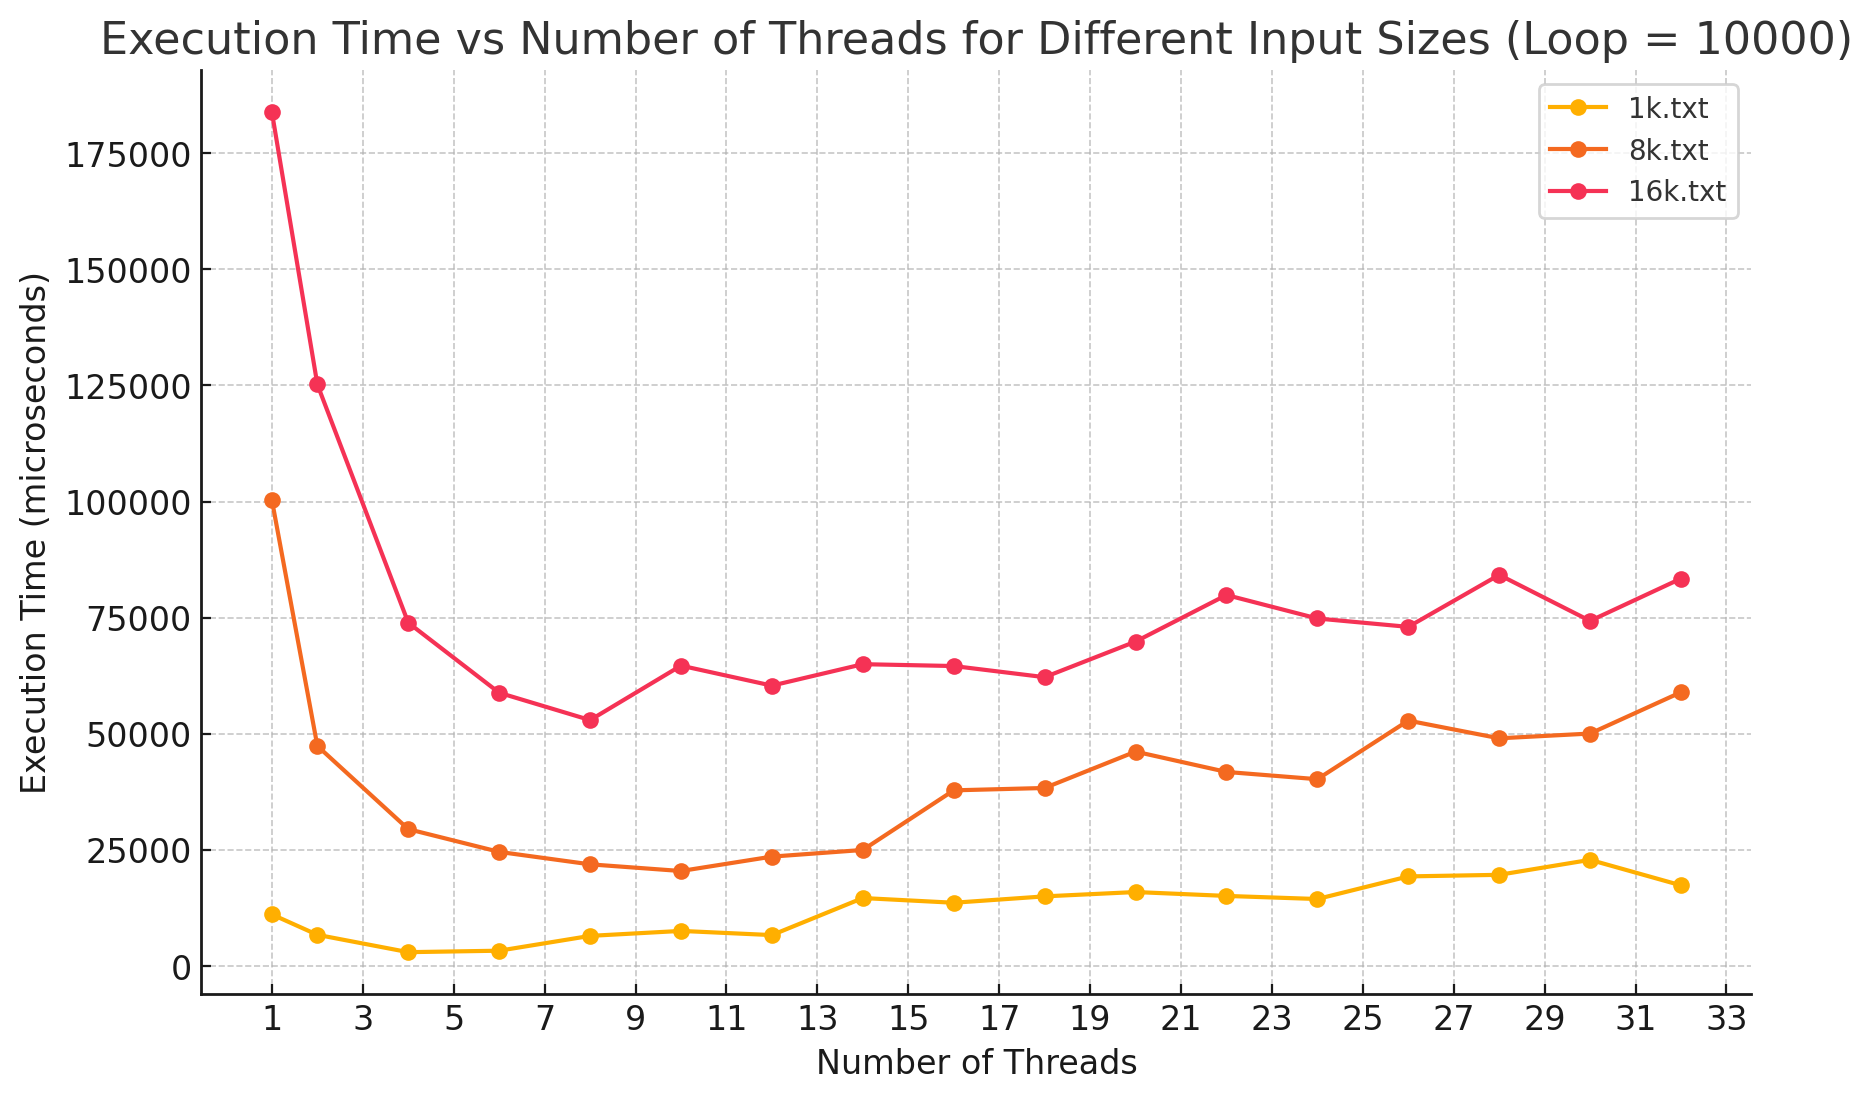
\includegraphics[width=\textwidth]{loop10000YieldExecutionTime.png}
        \caption{Number of Threads VS. Execution Time}
        \label{fig:ThreadVsExecutionTime}
    \end{subfigure}
    \caption{Speed-Up graph and Execution Time graph for loop = 10000}
    \label{fig:ThreadVsComparison}
\end{figure}
\hfill  % Horizontal space between figures


\begin{figure}[H]
    \centering
    \begin{subfigure}[t]{0.48\textwidth}  % Adjusted width for side-by-side
        \centering
        \includegraphics[width=\textwidth]{loop100000Yield.png}
        \caption{Number of Threads VS. Speed-Up}
        \label{fig:ThreadVsSpeedUp1}
    \end{subfigure}
    \hfill  % Horizontal space between figures
    \begin{subfigure}[t]{0.48\textwidth}  % Adjusted width for side-by-side
        \centering
        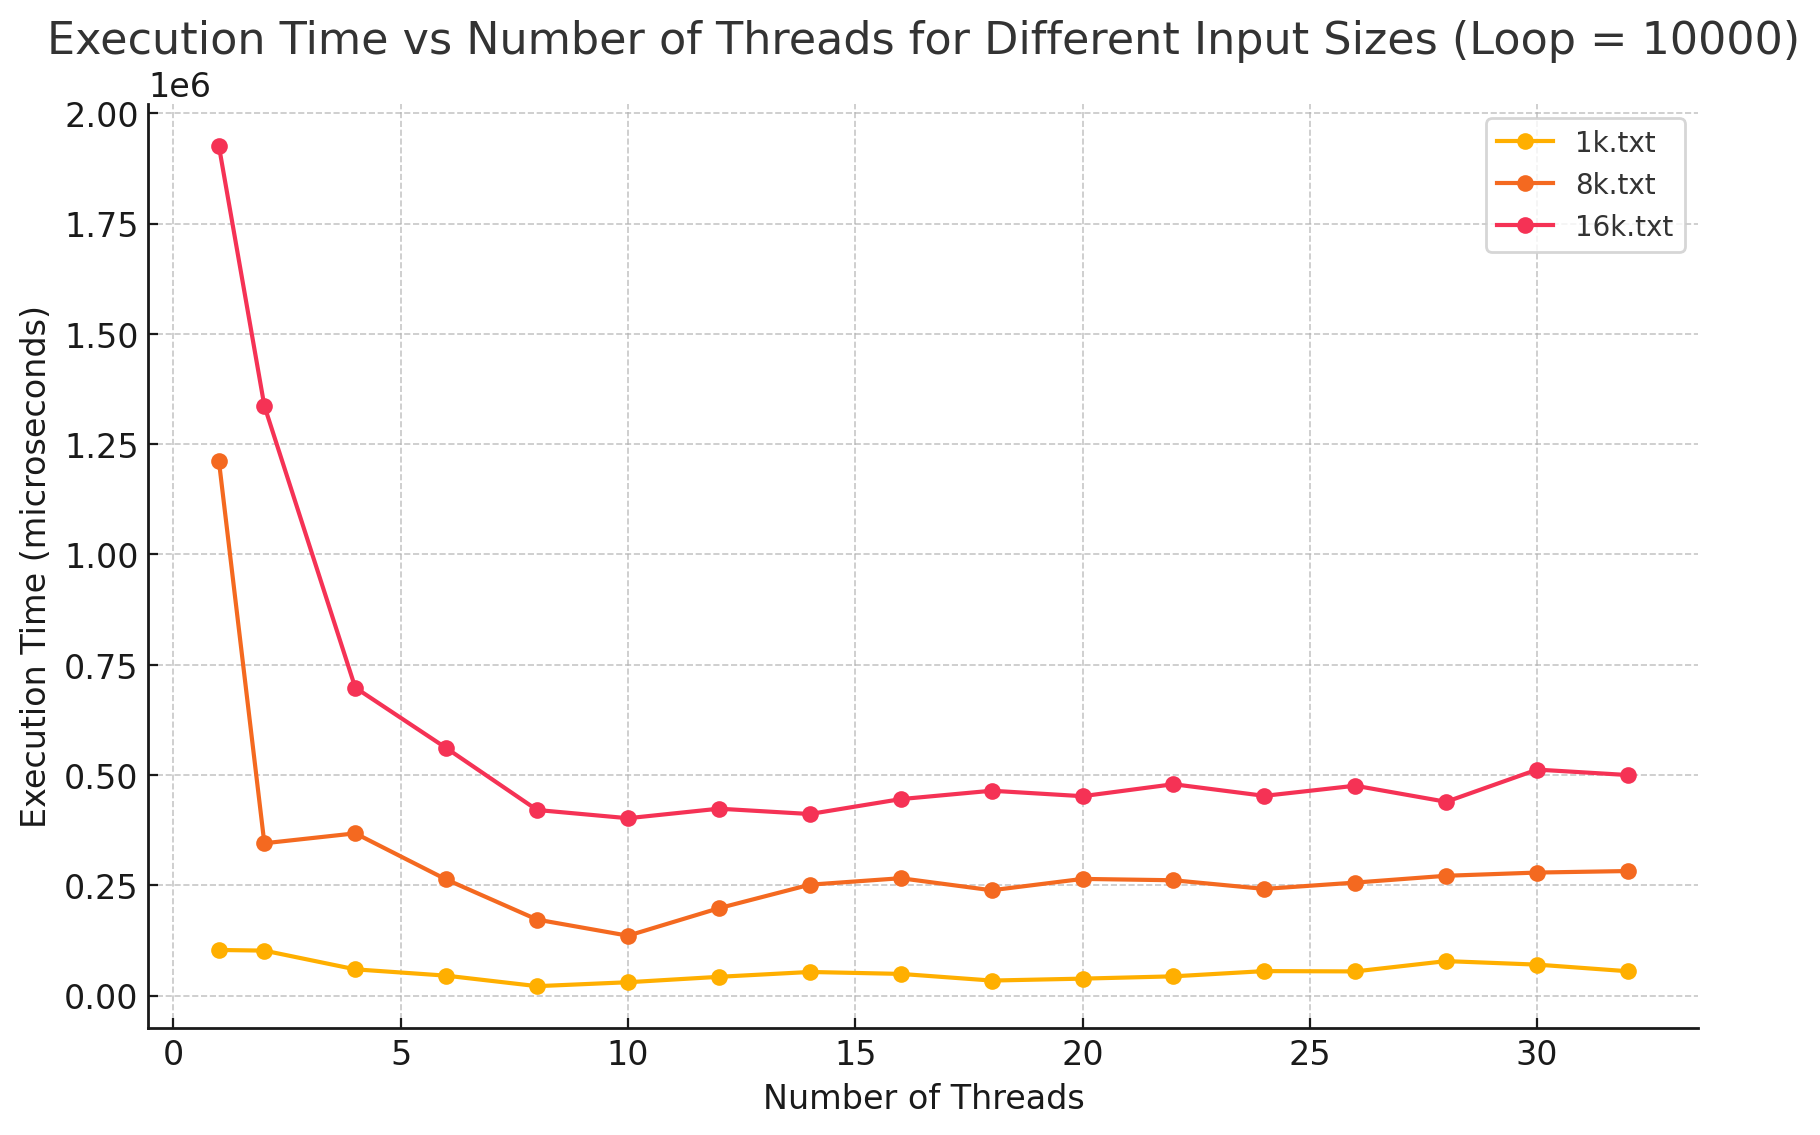
\includegraphics[width=\textwidth]{loop100000YieldExecutionTime.png}
        \caption{Number of Threads VS. Execution Time}
        \label{fig:ThreadVsExecutionTime}
    \end{subfigure}
    \caption{Speed-Up graph and Execution Time graph for loop = 100000}
    \label{fig:ThreadVsComparison}
\end{figure}



\subsection{Speedup analysis with Codio }
\begin{figure}[H]
    \centering
    \begin{subfigure}[t]{0.48\textwidth}  % Adjusted width for side-by-side
        \centering
        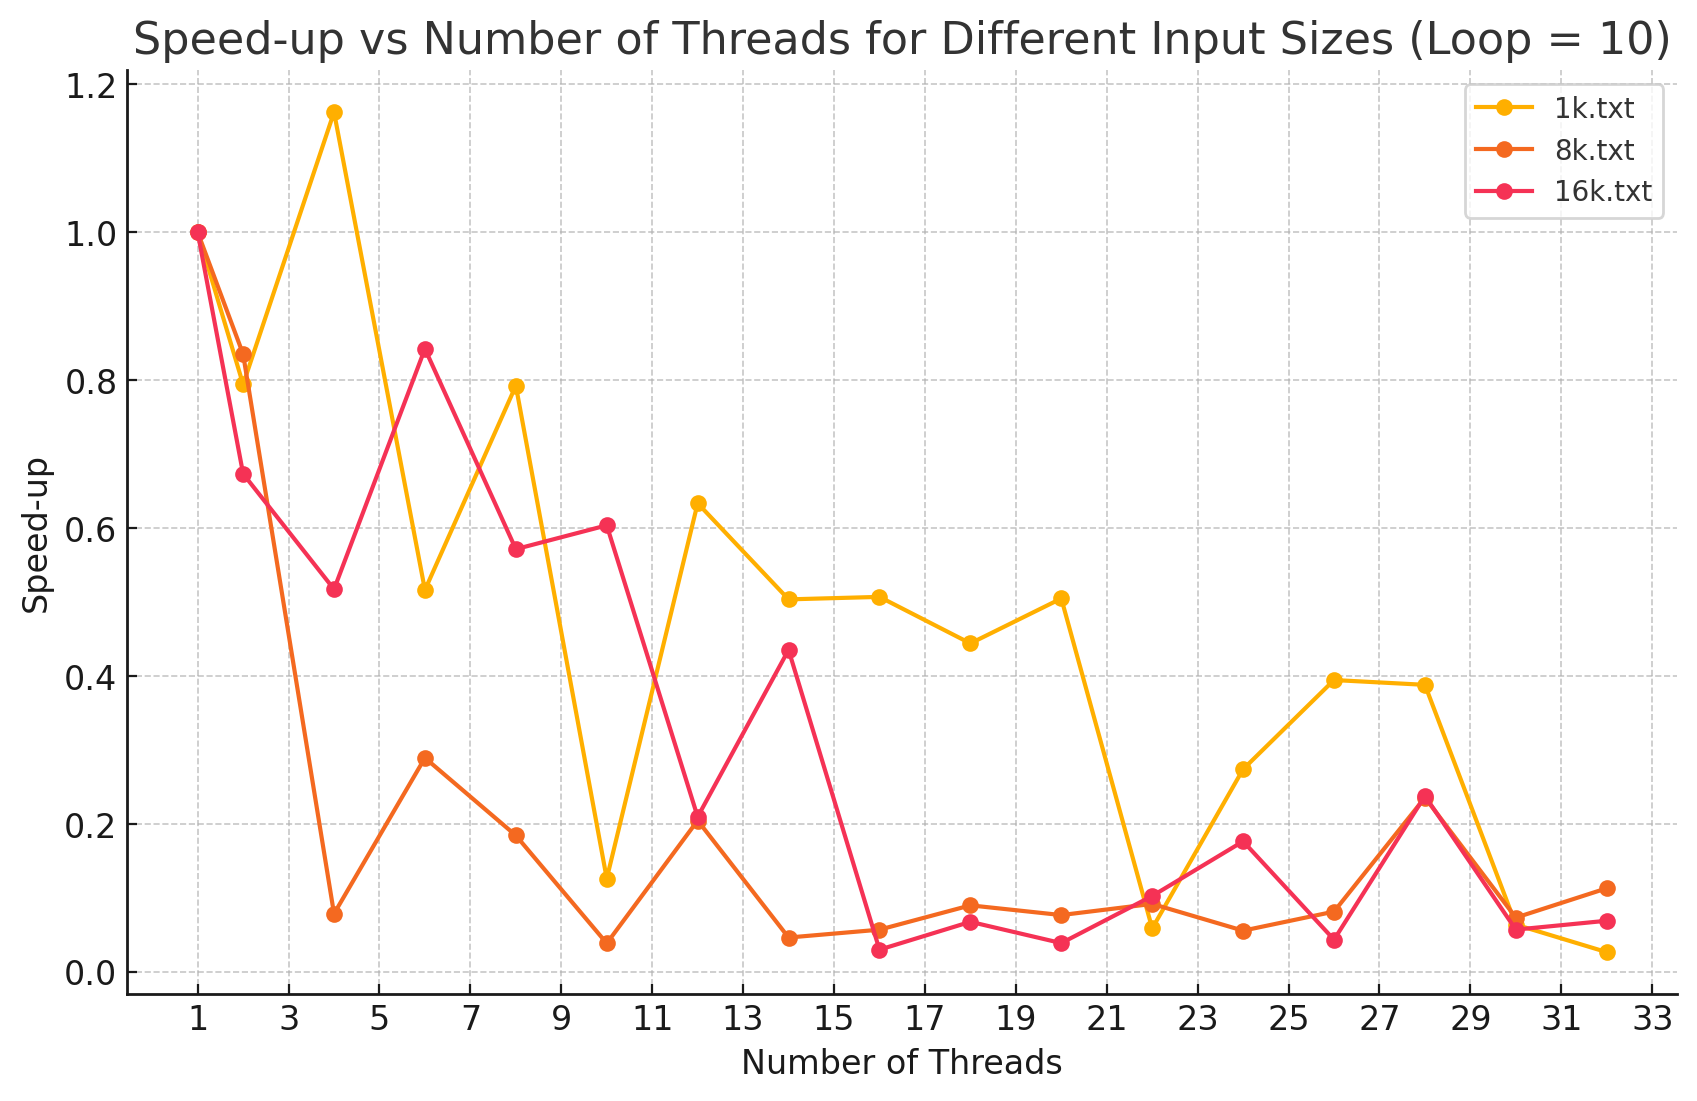
\includegraphics[width=\textwidth]{codioSleepLoop10.png}
        \caption{Number of Threads VS. Speed-Up}
        \label{fig:ThreadVsSpeedUp1}
    \end{subfigure}
    \hfill  % Horizontal space between figures
    \begin{subfigure}[t]{0.48\textwidth}  % Adjusted width for side-by-side
        \centering
        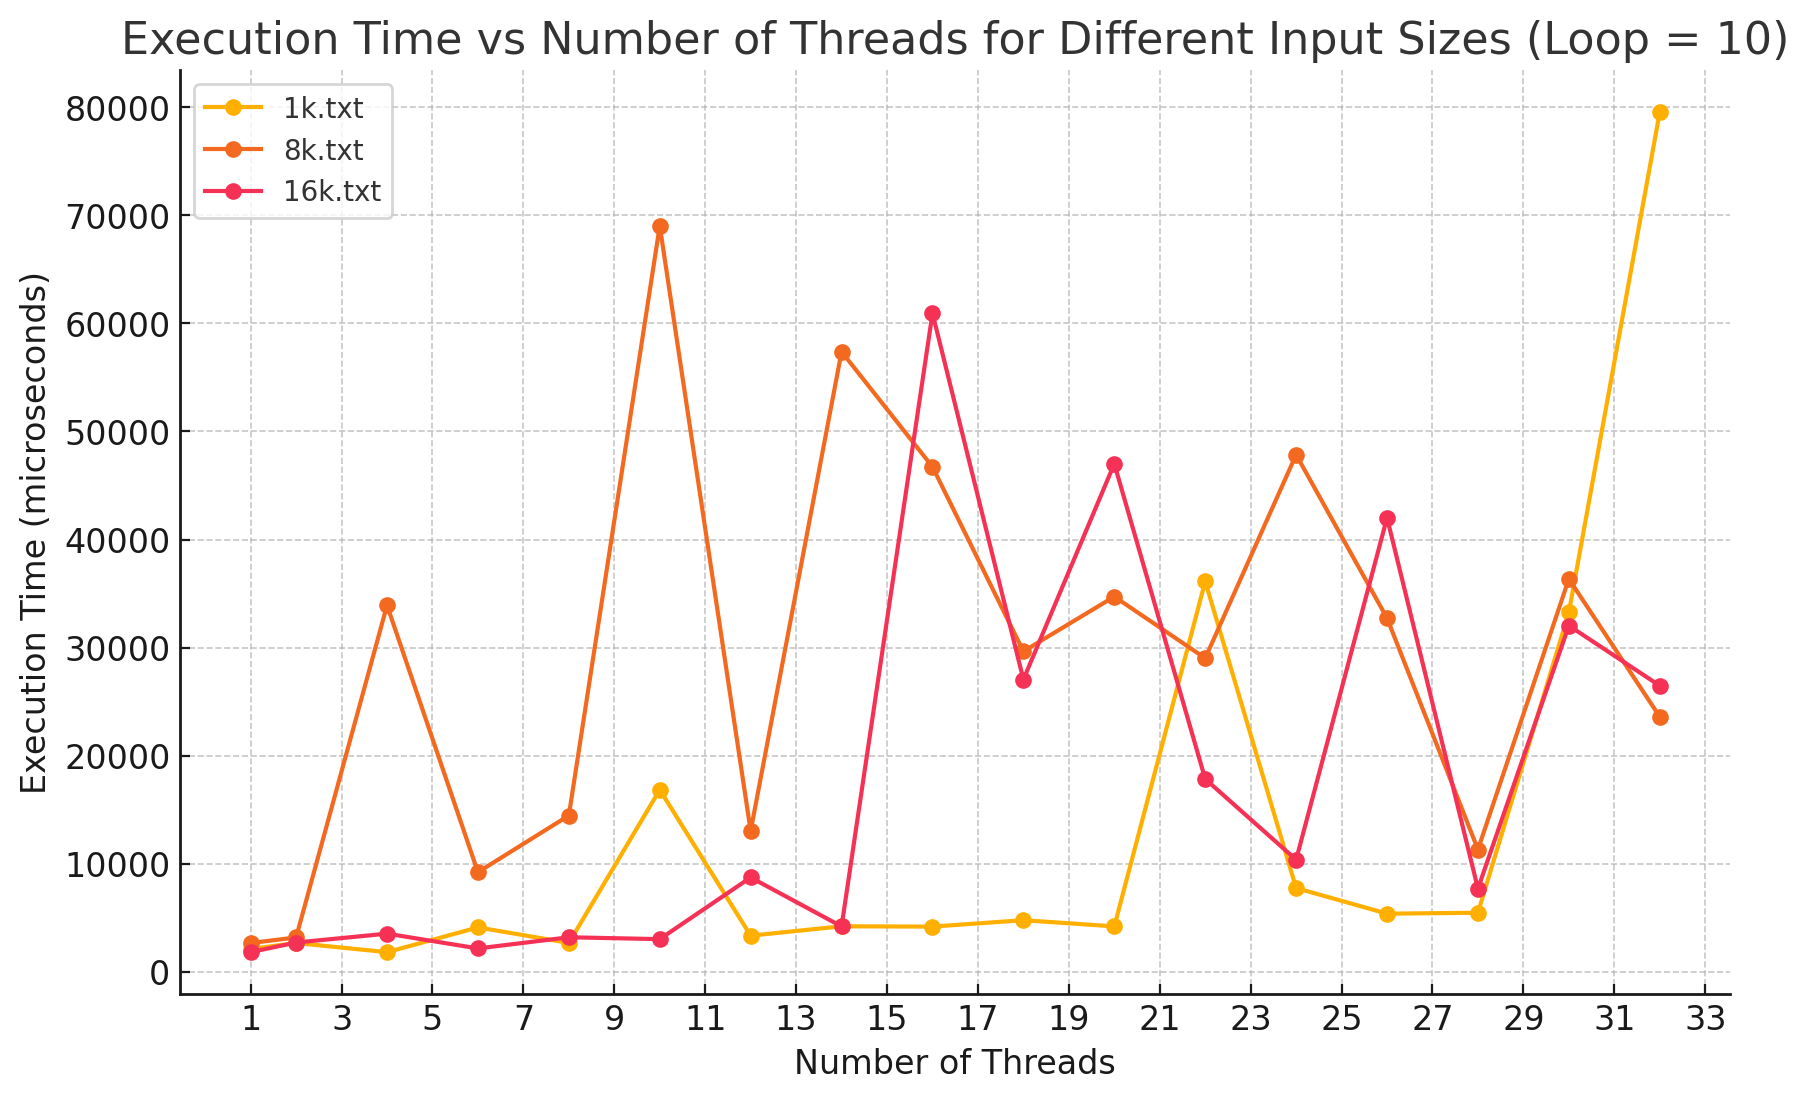
\includegraphics[width=\textwidth]{codioExecutionTimeLoop10.png}
        \caption{Number of Threads VS. Execution Time}
        \label{fig:ThreadVsExecutionTime}
    \end{subfigure}
    \caption{Speed-Up graph and Execution Time graph for loop = 10}
    \label{fig:ThreadVsComparison}
\end{figure}
\hfill  % Horizontal space between figures

\begin{figure}[H]
    \centering
    \begin{subfigure}[t]{0.48\textwidth}  % Adjusted width for side-by-side
        \centering
        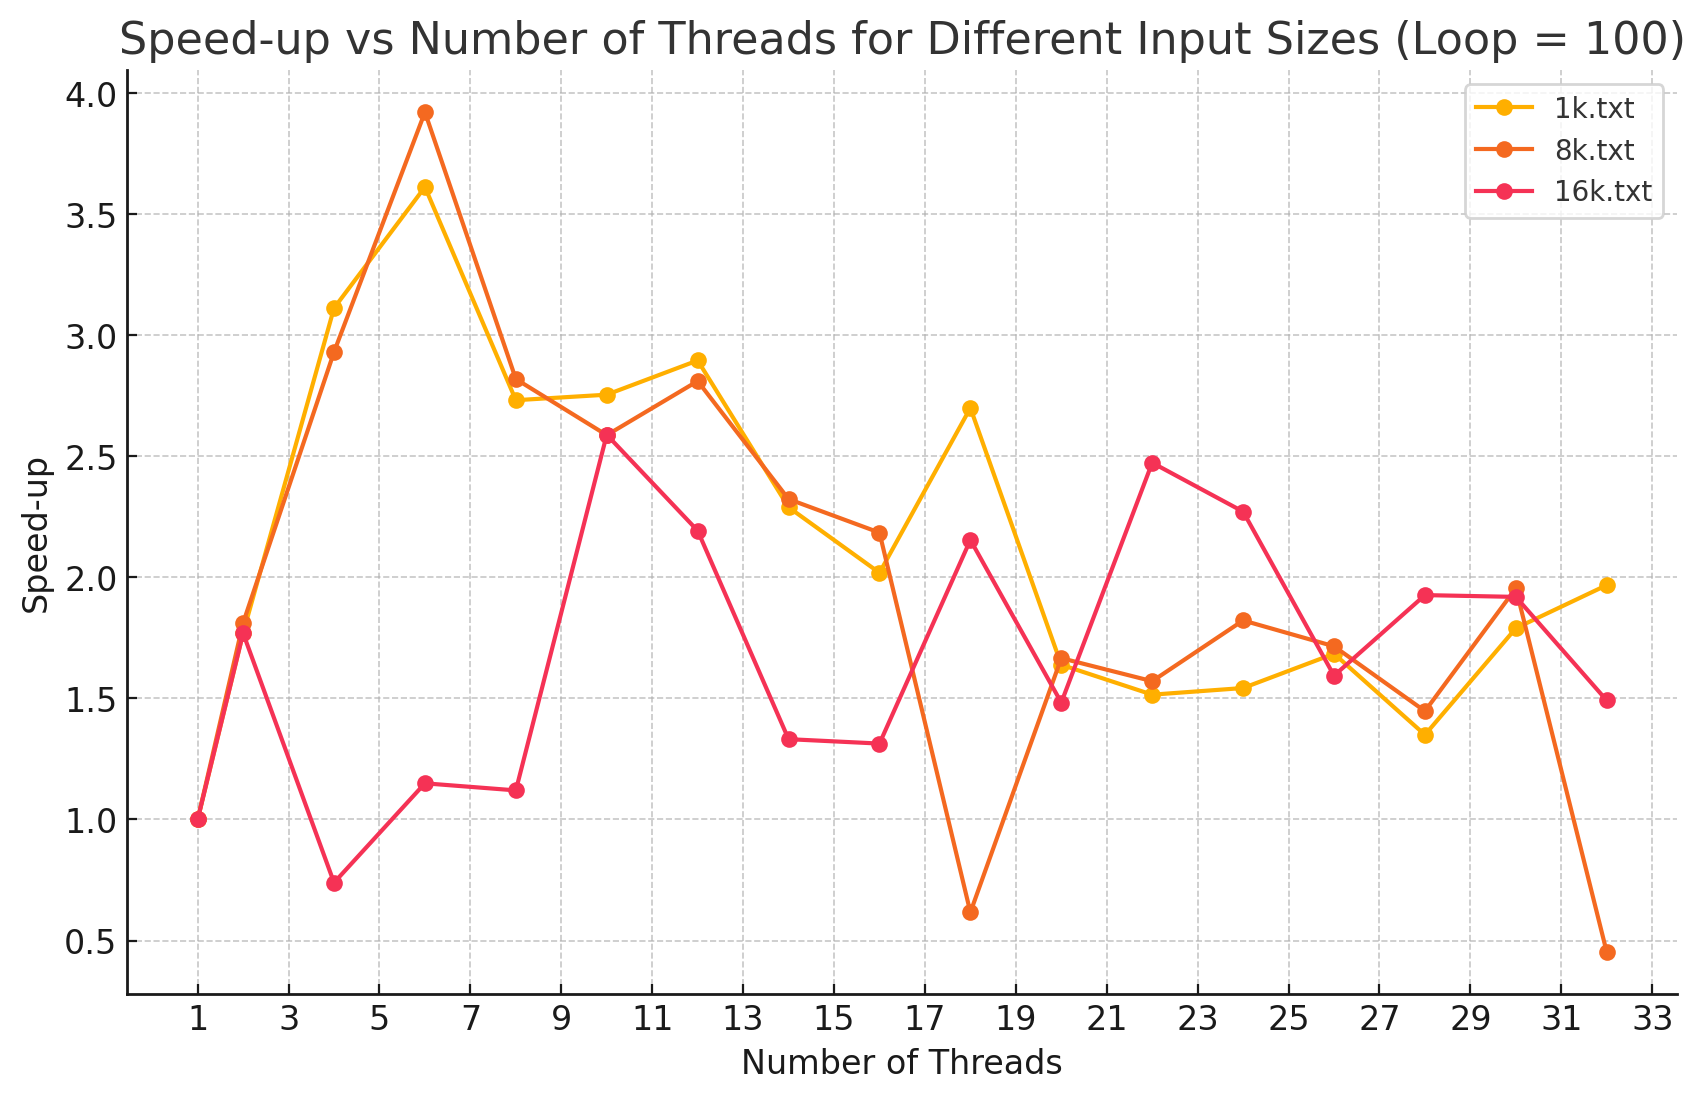
\includegraphics[width=\textwidth]{codioLoop100.png}
        \caption{Number of Threads VS. Speed-Up}
        \label{fig:ThreadVsSpeedUp1}
    \end{subfigure}
    \hfill  % Horizontal space between figures
    \begin{subfigure}[t]{0.48\textwidth}  % Adjusted width for side-by-side
        \centering
        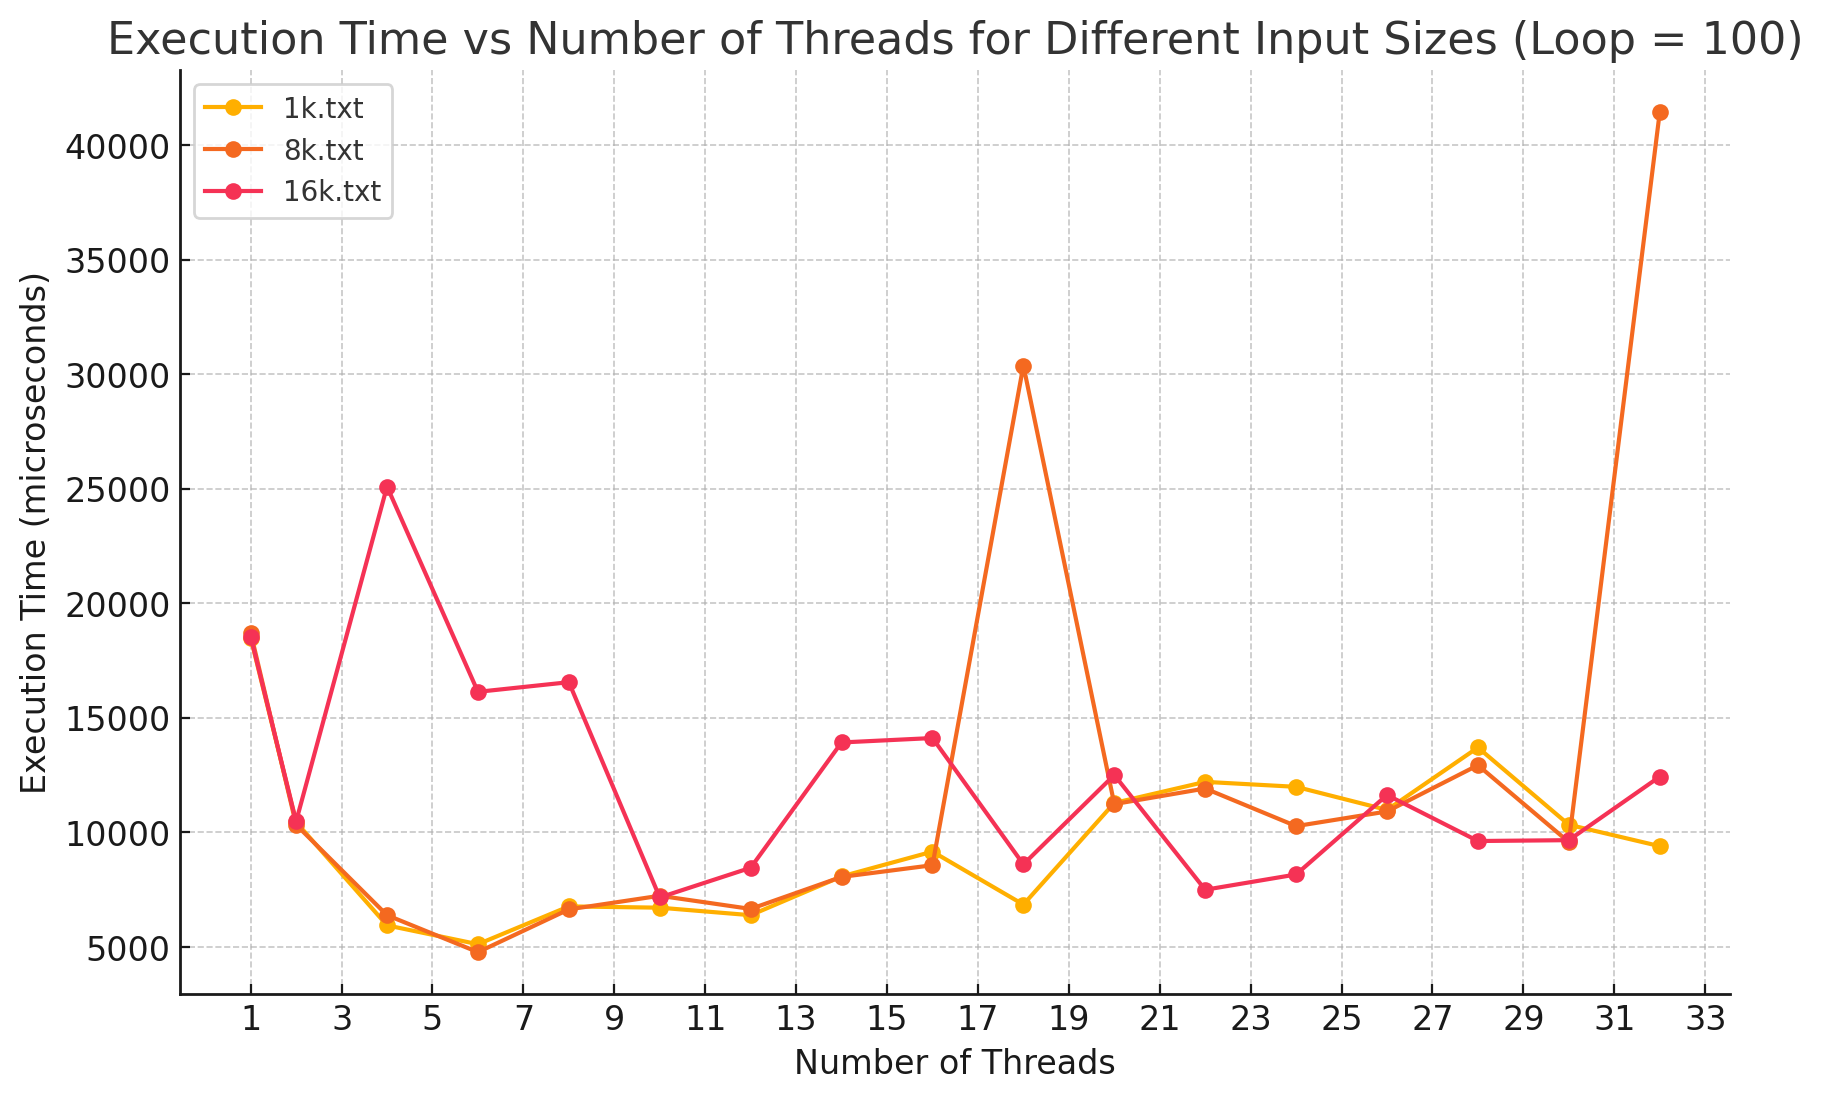
\includegraphics[width=\textwidth]{codioExecutionTimeLoop100.png}
        \caption{Number of Threads VS. Execution Time}
        \label{fig:ThreadVsExecutionTime}
    \end{subfigure}
    \caption{Speed-Up graph and Execution Time graph for loop = 100}
    \label{fig:ThreadVsComparison}
\end{figure}
\hfill  % Horizontal space between figures

\begin{figure}[H]
    \centering
    \begin{subfigure}[t]{0.48\textwidth}  % Adjusted width for side-by-side
        \centering
        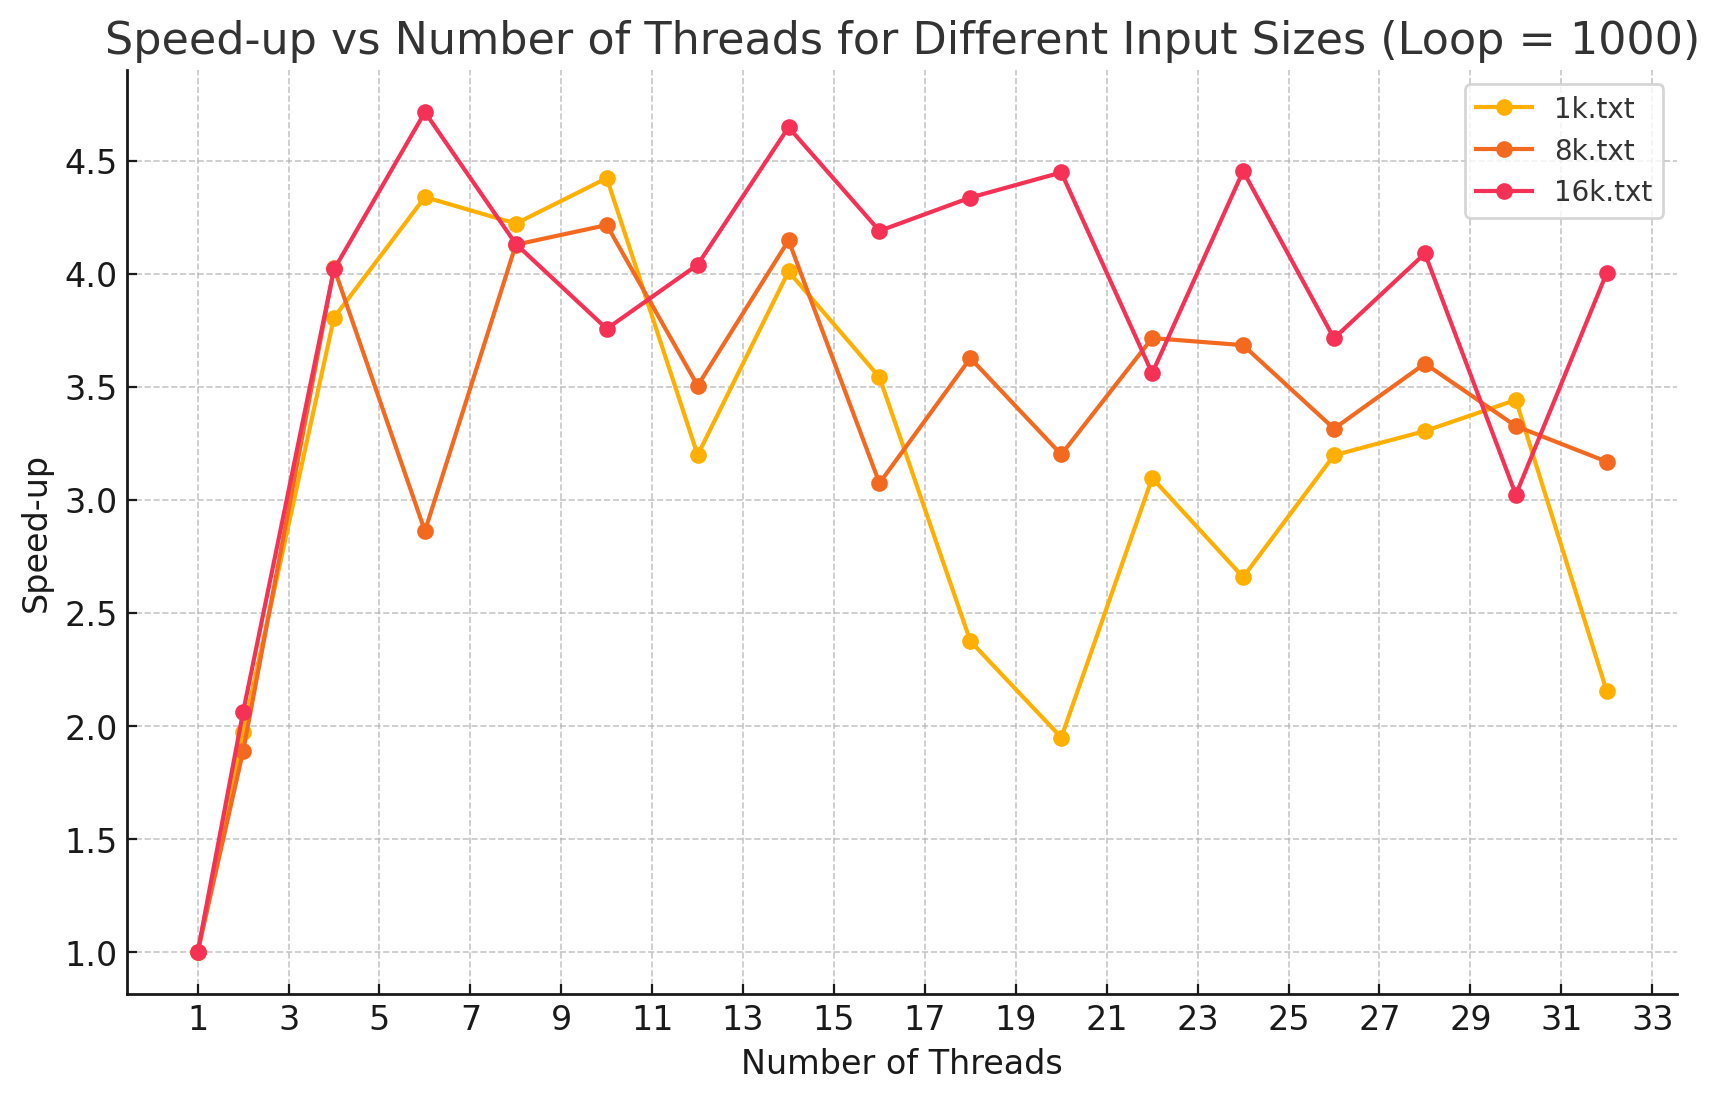
\includegraphics[width=\textwidth]{codioLoop1000.png}
        \caption{Number of Threads VS. Speed-Up}
        \label{fig:ThreadVsSpeedUp1}
    \end{subfigure}
    \hfill  % Horizontal space between figures
    \begin{subfigure}[t]{0.48\textwidth}  % Adjusted width for side-by-side
        \centering
        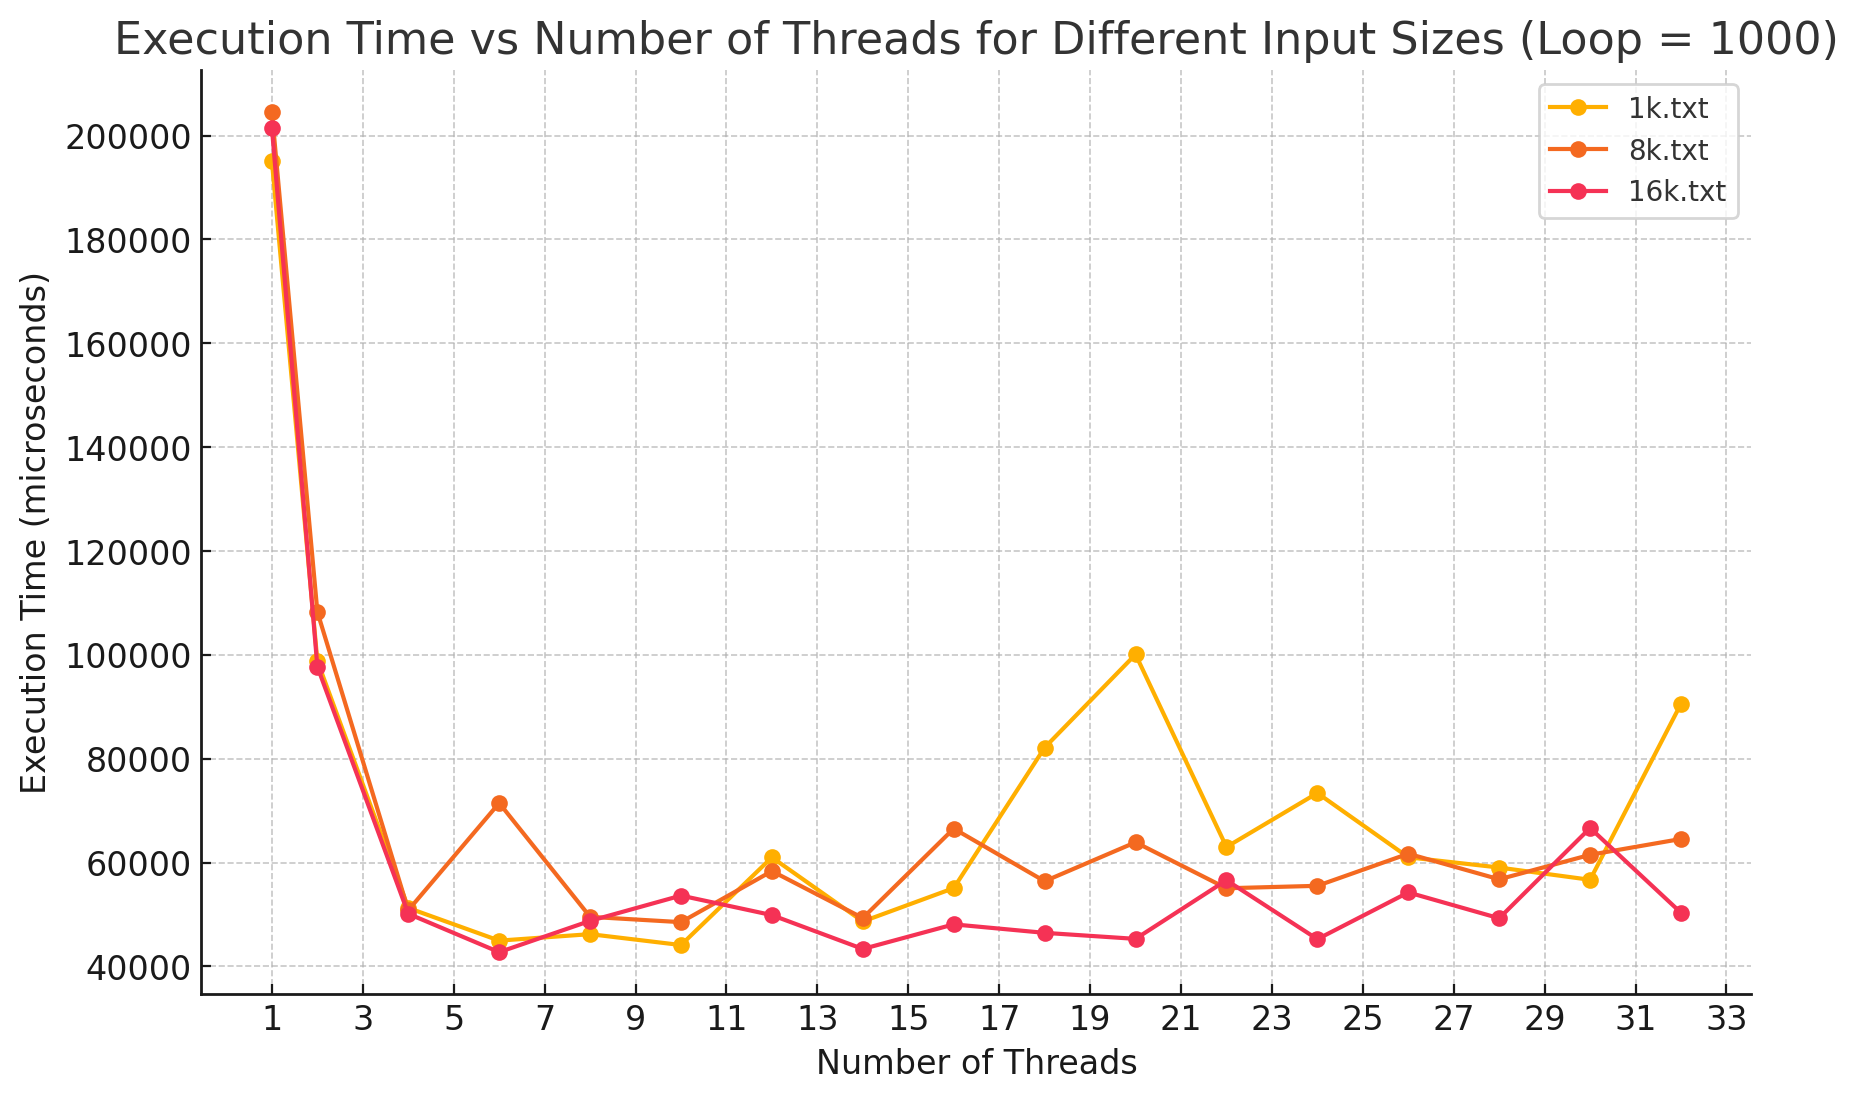
\includegraphics[width=\textwidth]{codioExecutionTimeLoop1000.png}
        \caption{Number of Threads VS. Execution Time}
        \label{fig:ThreadVsExecutionTime}
    \end{subfigure}
    \caption{Speed-Up graph and Execution Time graph for loop = 1000}
    \label{fig:ThreadVsComparison}
\end{figure}
\hfill  % Horizontal space between figures


\begin{figure}[H]
    \centering
    \begin{subfigure}[t]{0.48\textwidth}  % Adjusted width for side-by-side
        \centering
        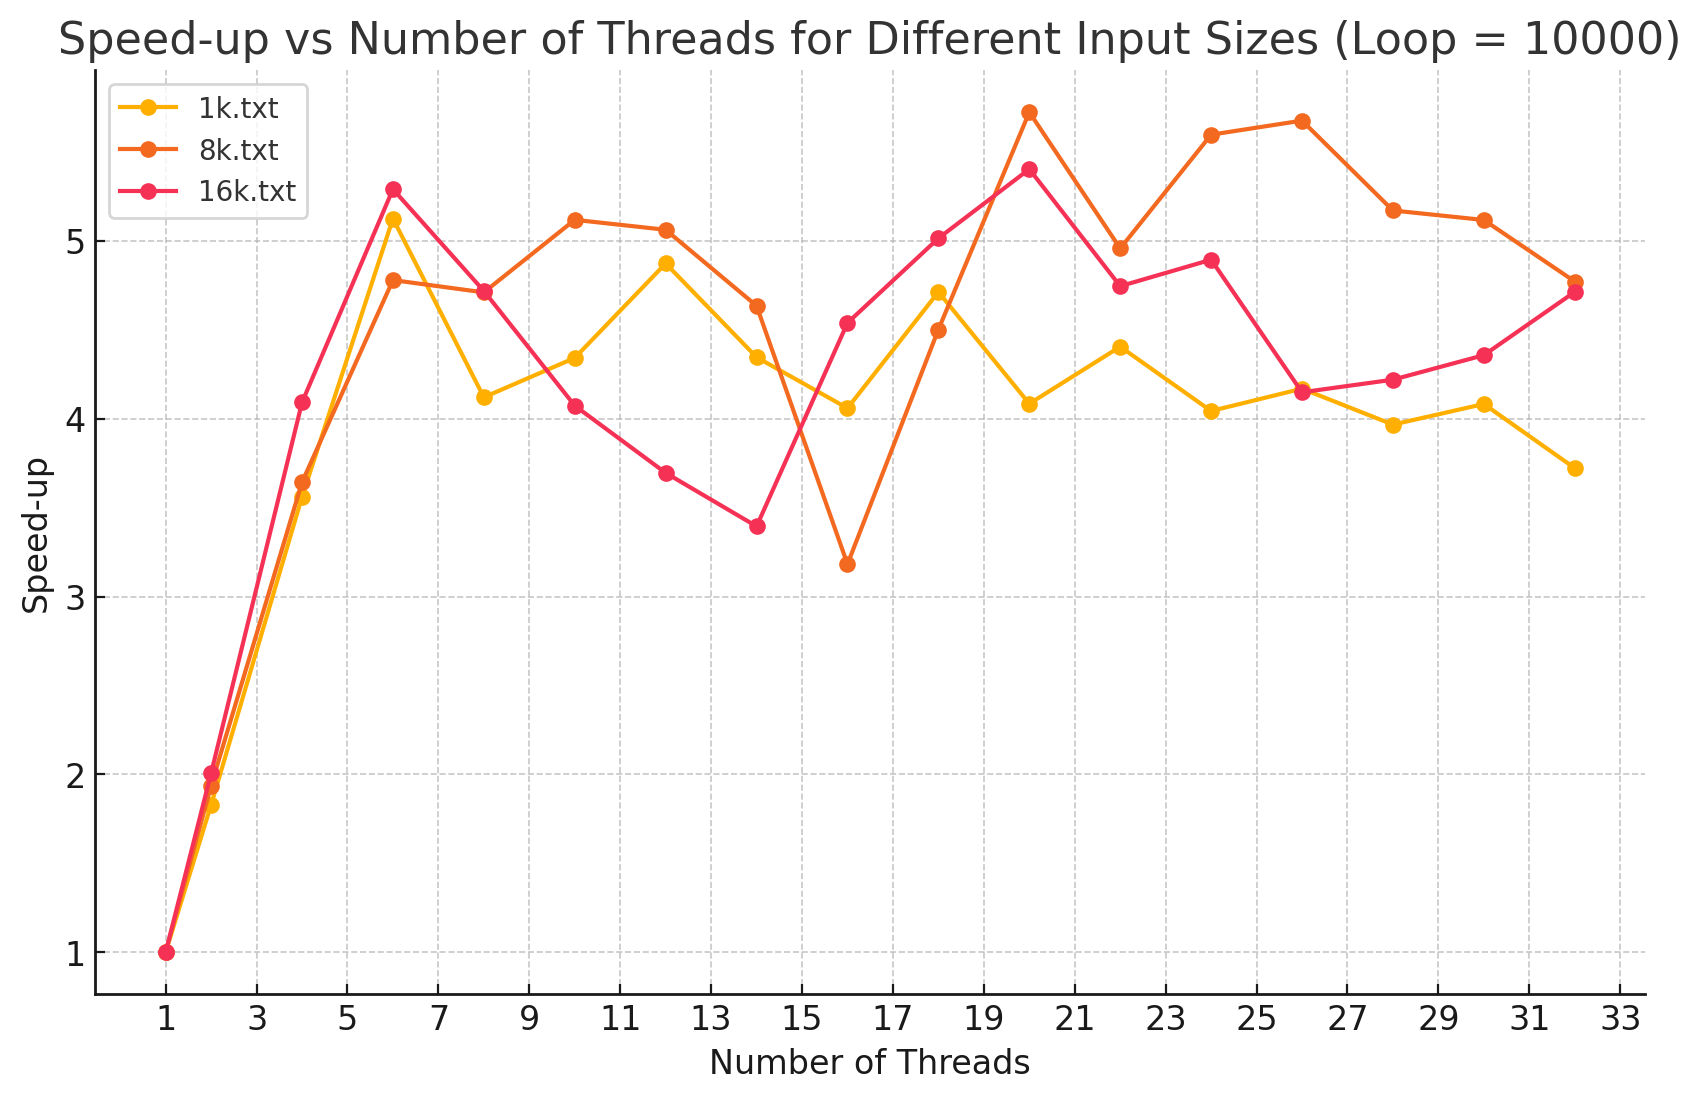
\includegraphics[width=\textwidth]{codioWithSleepLoop10000.png}
        \caption{Number of Threads VS. Speed-Up}
        \label{fig:ThreadVsSpeedUp1}
    \end{subfigure}
    \hfill  % Horizontal space between figures
    \begin{subfigure}[t]{0.48\textwidth}  % Adjusted width for side-by-side
        \centering
        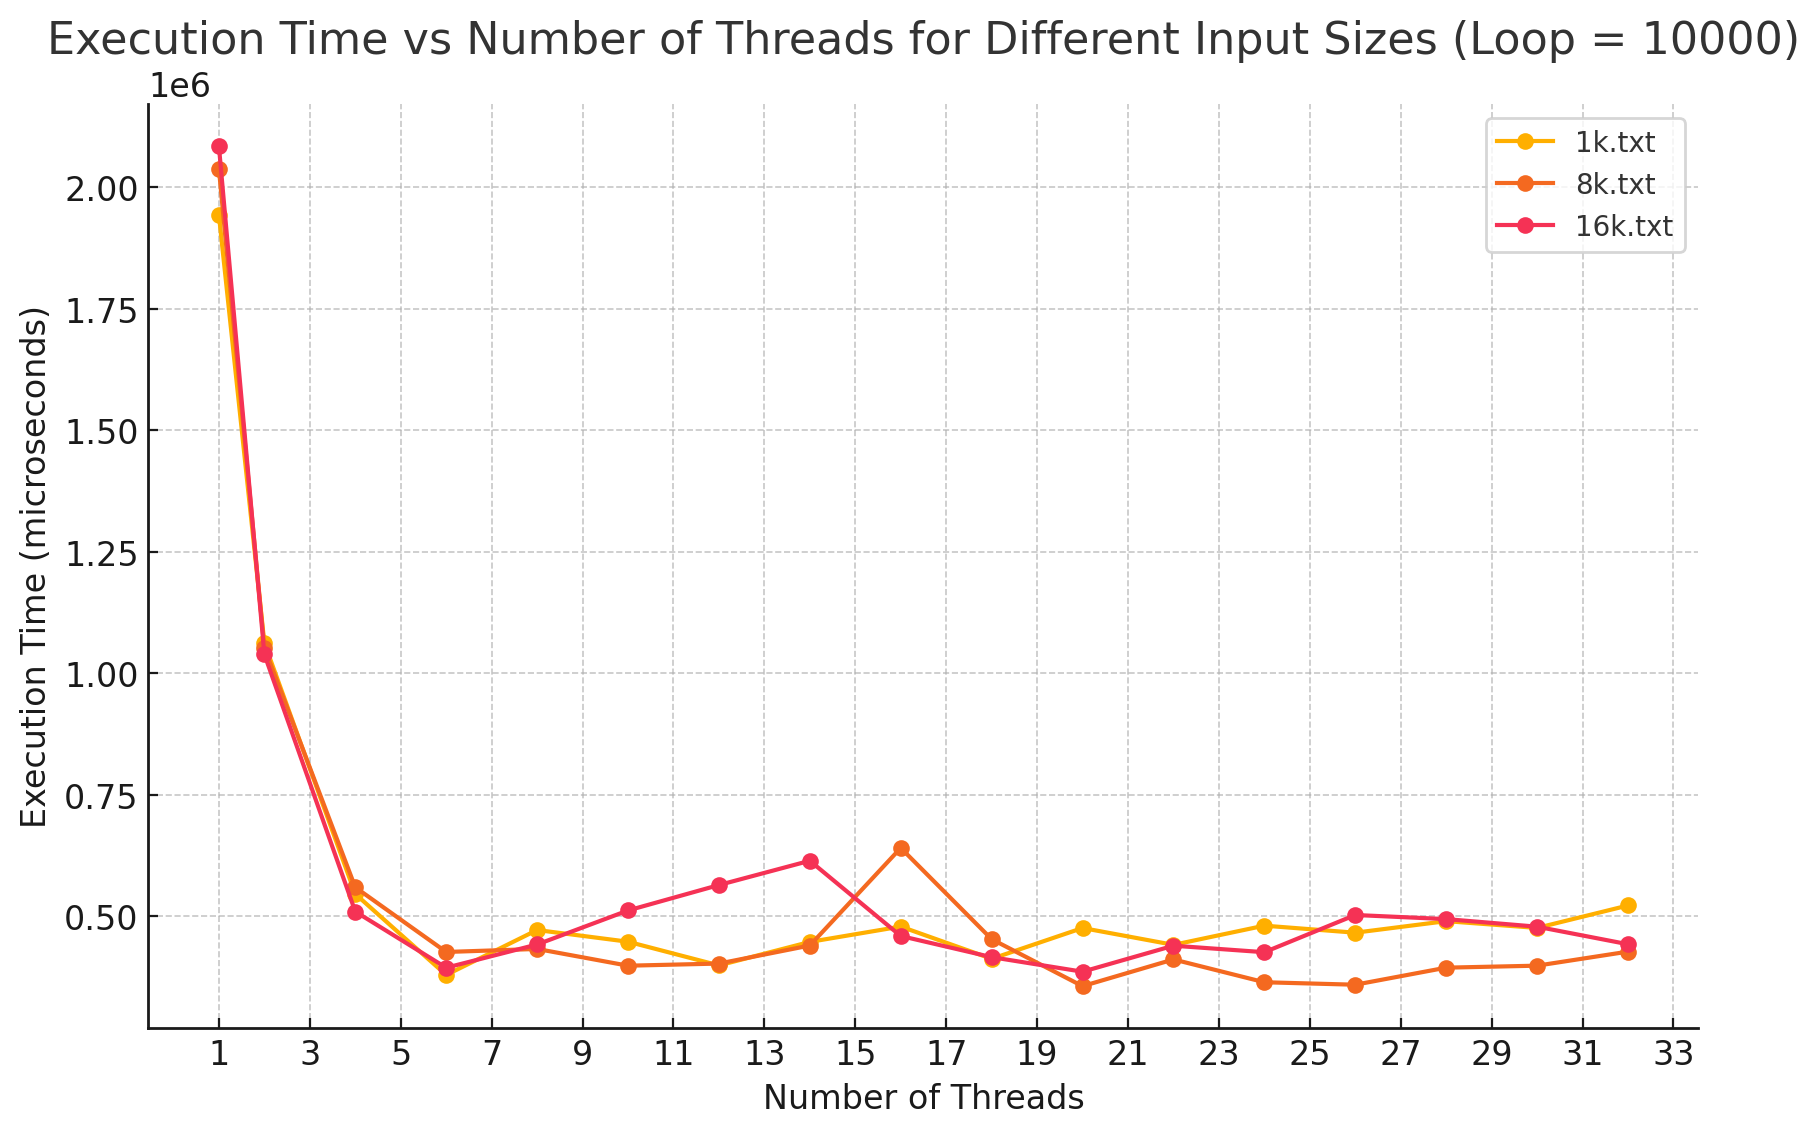
\includegraphics[width=\textwidth]{codioExecutionTimeLoop10000.png}
        \caption{Number of Threads VS. Execution Time}
        \label{fig:ThreadVsExecutionTime}
    \end{subfigure}
    \caption{Speed-Up graph and Execution Time graph for loop = 10000}
    \label{fig:ThreadVsComparison}
\end{figure}
\hfill  % Horizontal space between figures



\begin{figure}[H]
    \centering
    \begin{subfigure}[t]{0.48\textwidth}  % Adjusted width for side-by-side
        \centering
        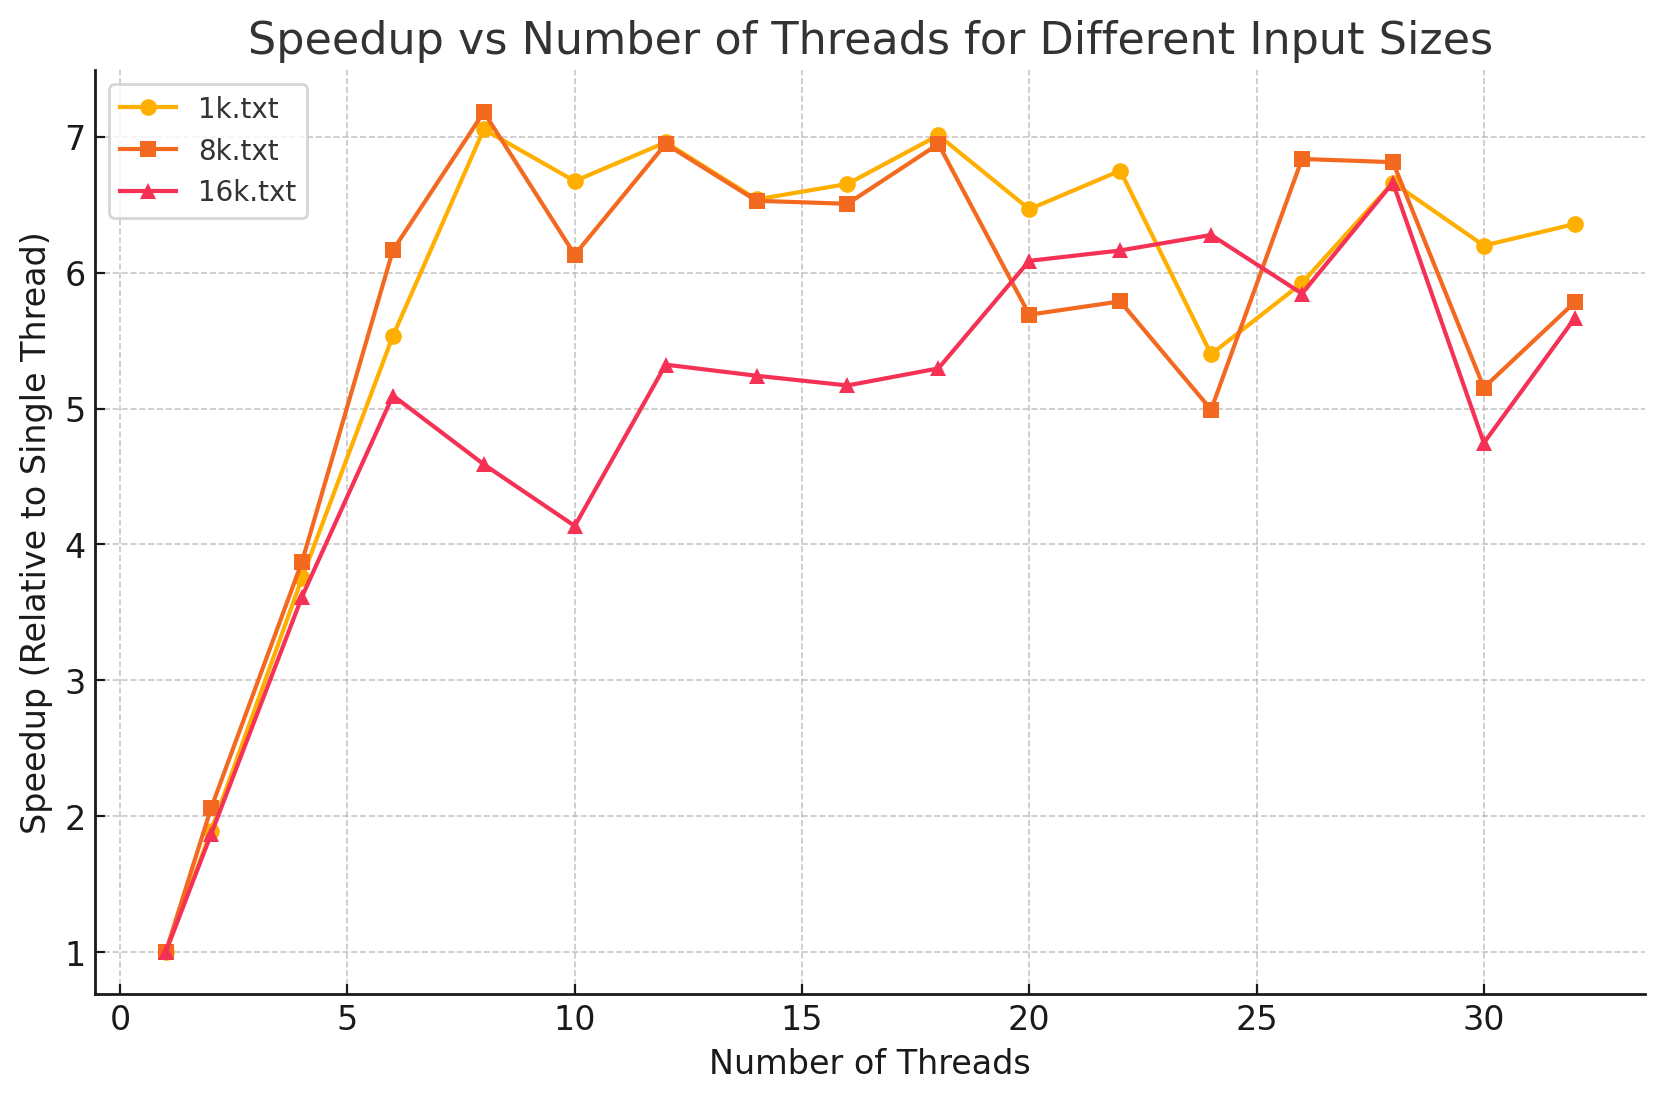
\includegraphics[width=\textwidth]{codioWithSleepLoop100000.png}
        \caption{Number of Threads VS. Speed-Up}
        \label{fig:ThreadVsSpeedUp1}
    \end{subfigure}
    \hfill  % Horizontal space between figures
    \begin{subfigure}[t]{0.48\textwidth}  % Adjusted width for side-by-side
        \centering
        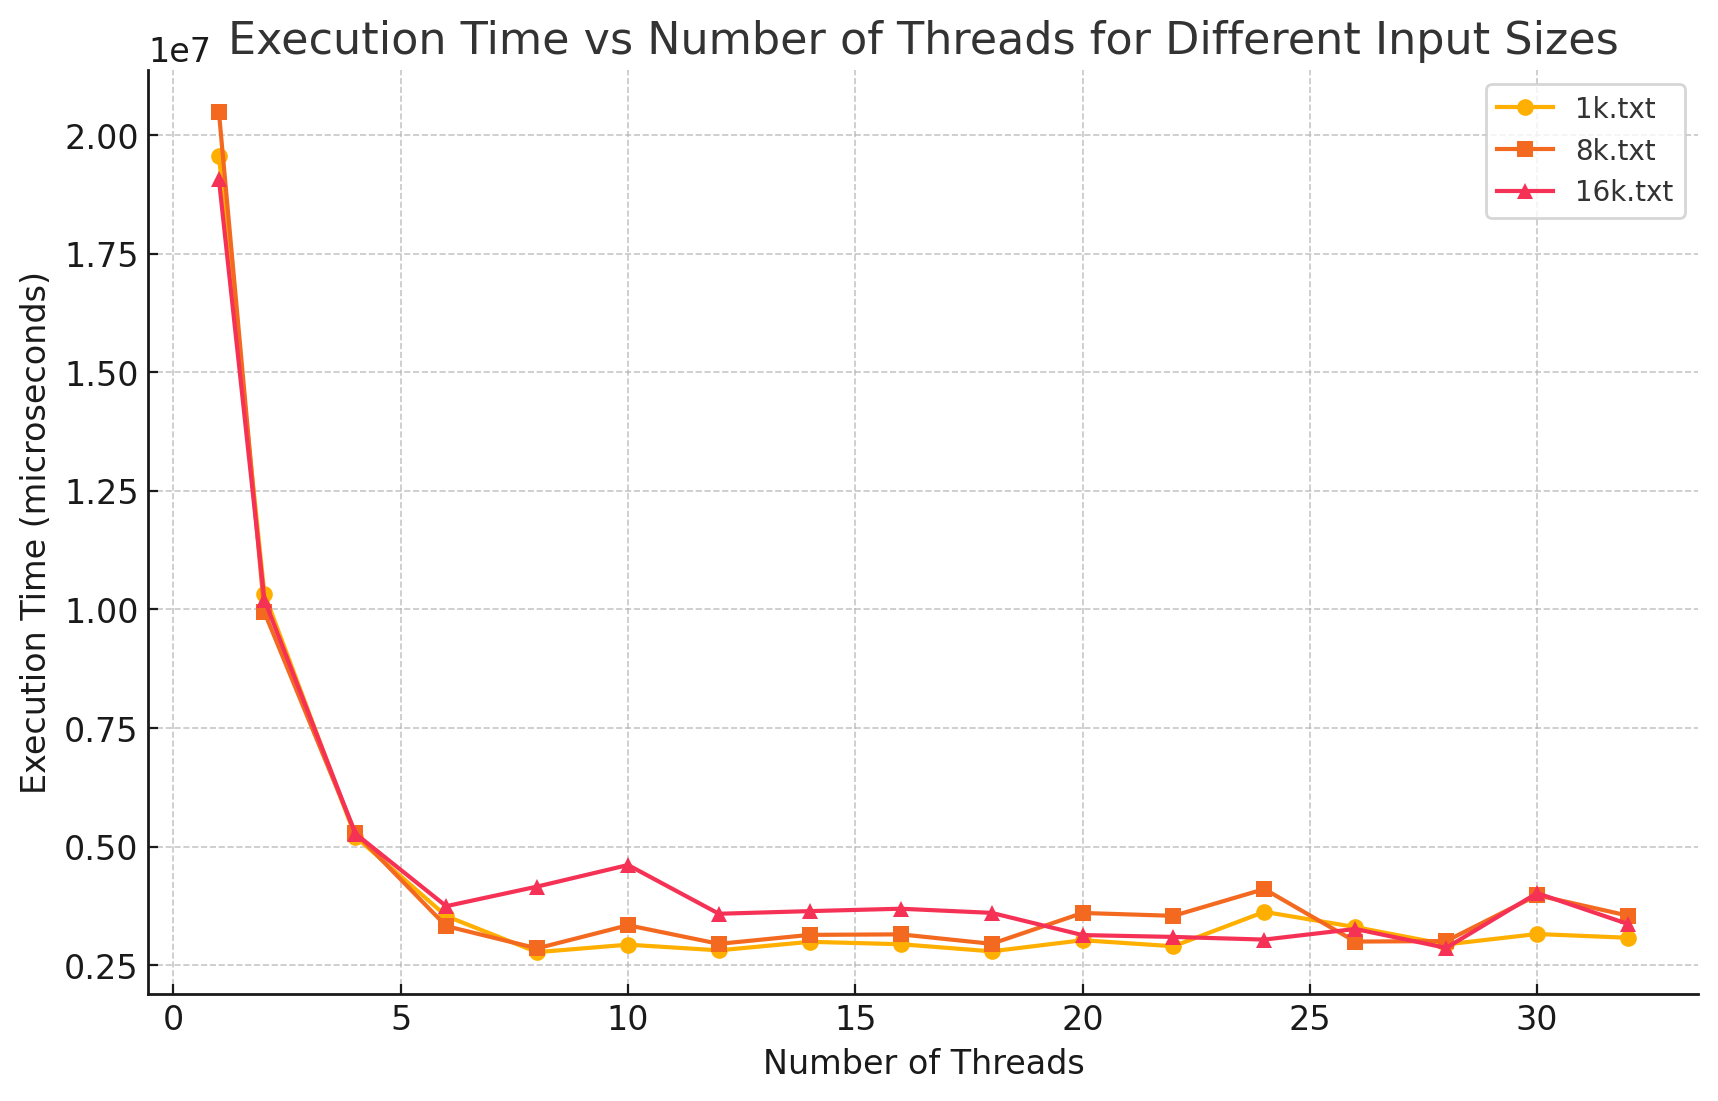
\includegraphics[width=\textwidth]{codioExecutionTimeLoop100000.png}
        \caption{Number of Threads VS. Execution Time}
        \label{fig:ThreadVsExecutionTime}
    \end{subfigure}
    \caption{Speed-Up graph and Execution Time graph for loop = 100000}
    \label{fig:ThreadVsComparison}
\end{figure}
\hfill  % Horizontal space between figures


\subsection{Speedup analysis with addition as operator (Comparison group) }

\begin{figure}[H]
    \centering
    \begin{subfigure}[t]{0.48\textwidth}  % Adjusted width for side-by-side
        \centering
        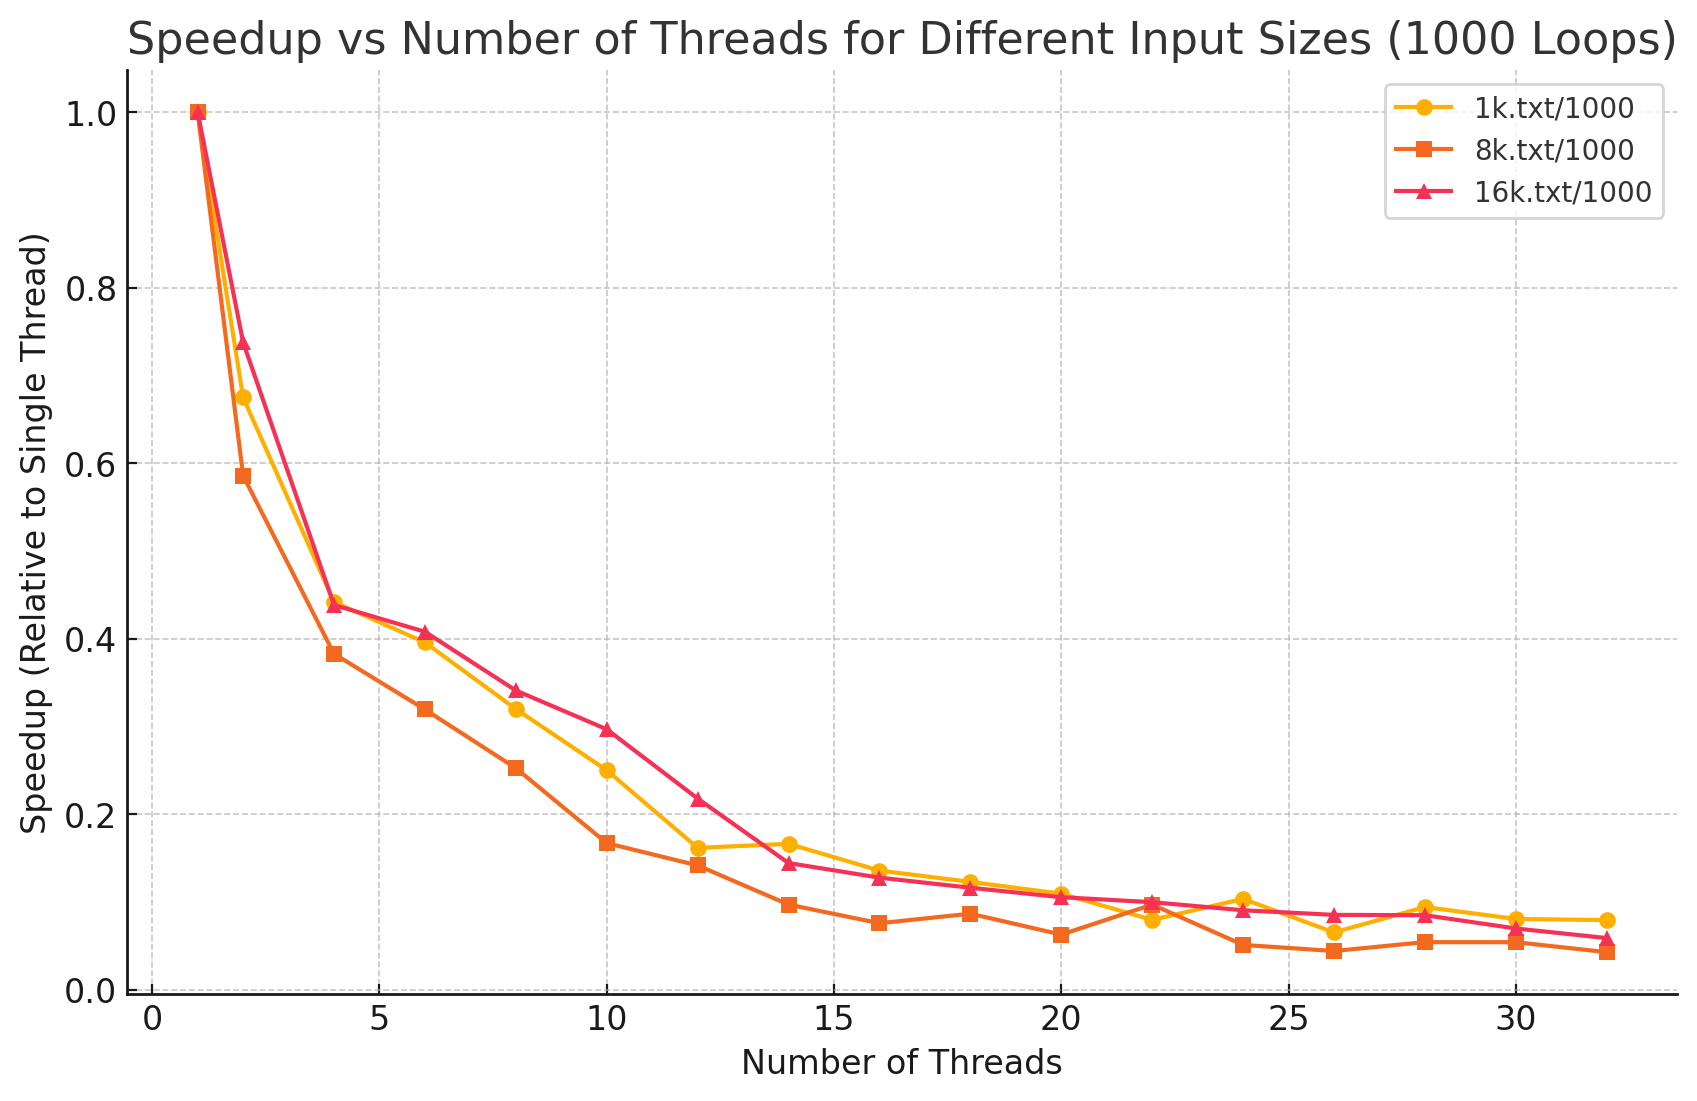
\includegraphics[width=\textwidth]{additionAsOpLoop1000Speedup.png}
        \caption{Number of Threads VS. Speed-Up}
        \label{fig:ThreadVsSpeedUp1}
    \end{subfigure}
    \hfill  % Horizontal space between figures
    \begin{subfigure}[t]{0.48\textwidth}  % Adjusted width for side-by-side
        \centering
        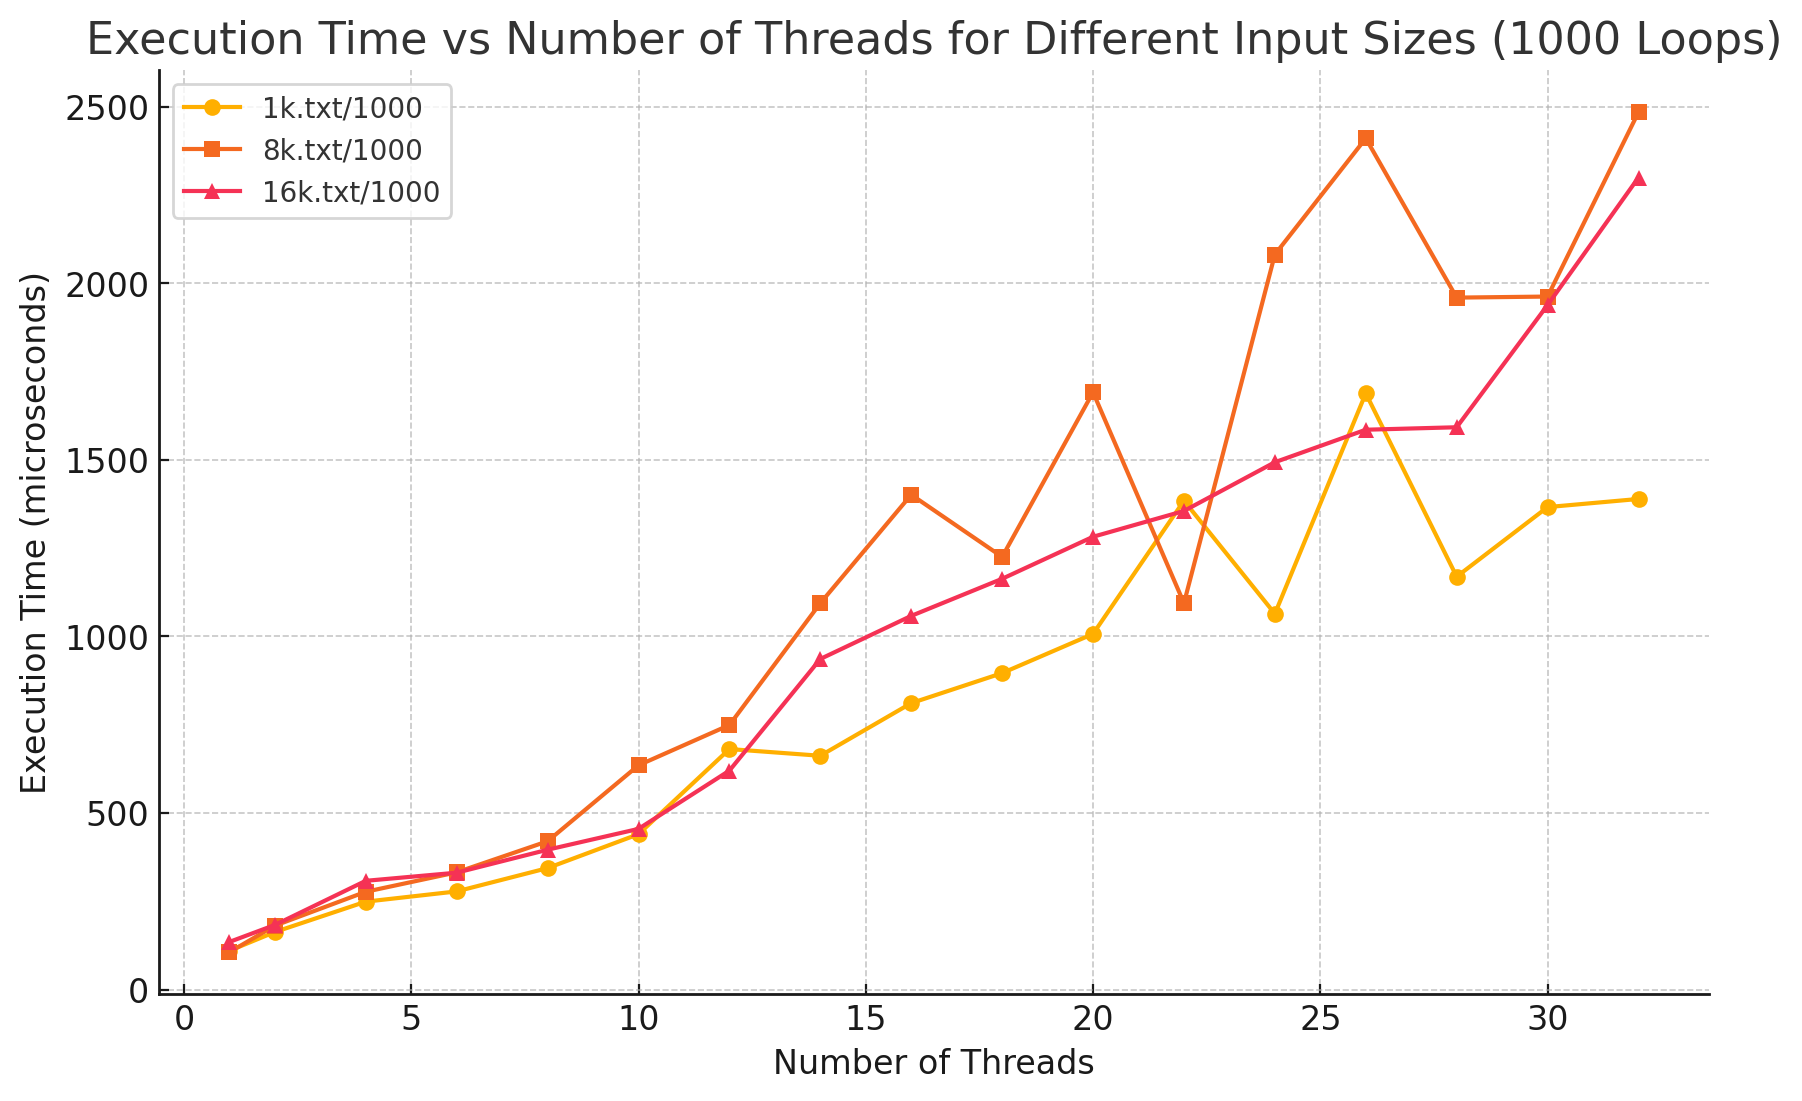
\includegraphics[width=\textwidth]{additionAsOpLoop1000Exe.png}
        \caption{Number of Threads VS. Execution Time}
        \label{fig:ThreadVsExecutionTime}
    \end{subfigure}
    \caption{Speed-Up graph and Execution Time graph for loop = 1000}
    \label{fig:ThreadVsComparison}
\end{figure}
\hfill  % Horizontal space between figures

\subsection{Speedup analysis with pthread\_barrier\_wait (Comparison group) }

\begin{figure}[H]
    \centering
    \begin{subfigure}[t]{0.48\textwidth}  % Adjusted width for side-by-side
        \centering
        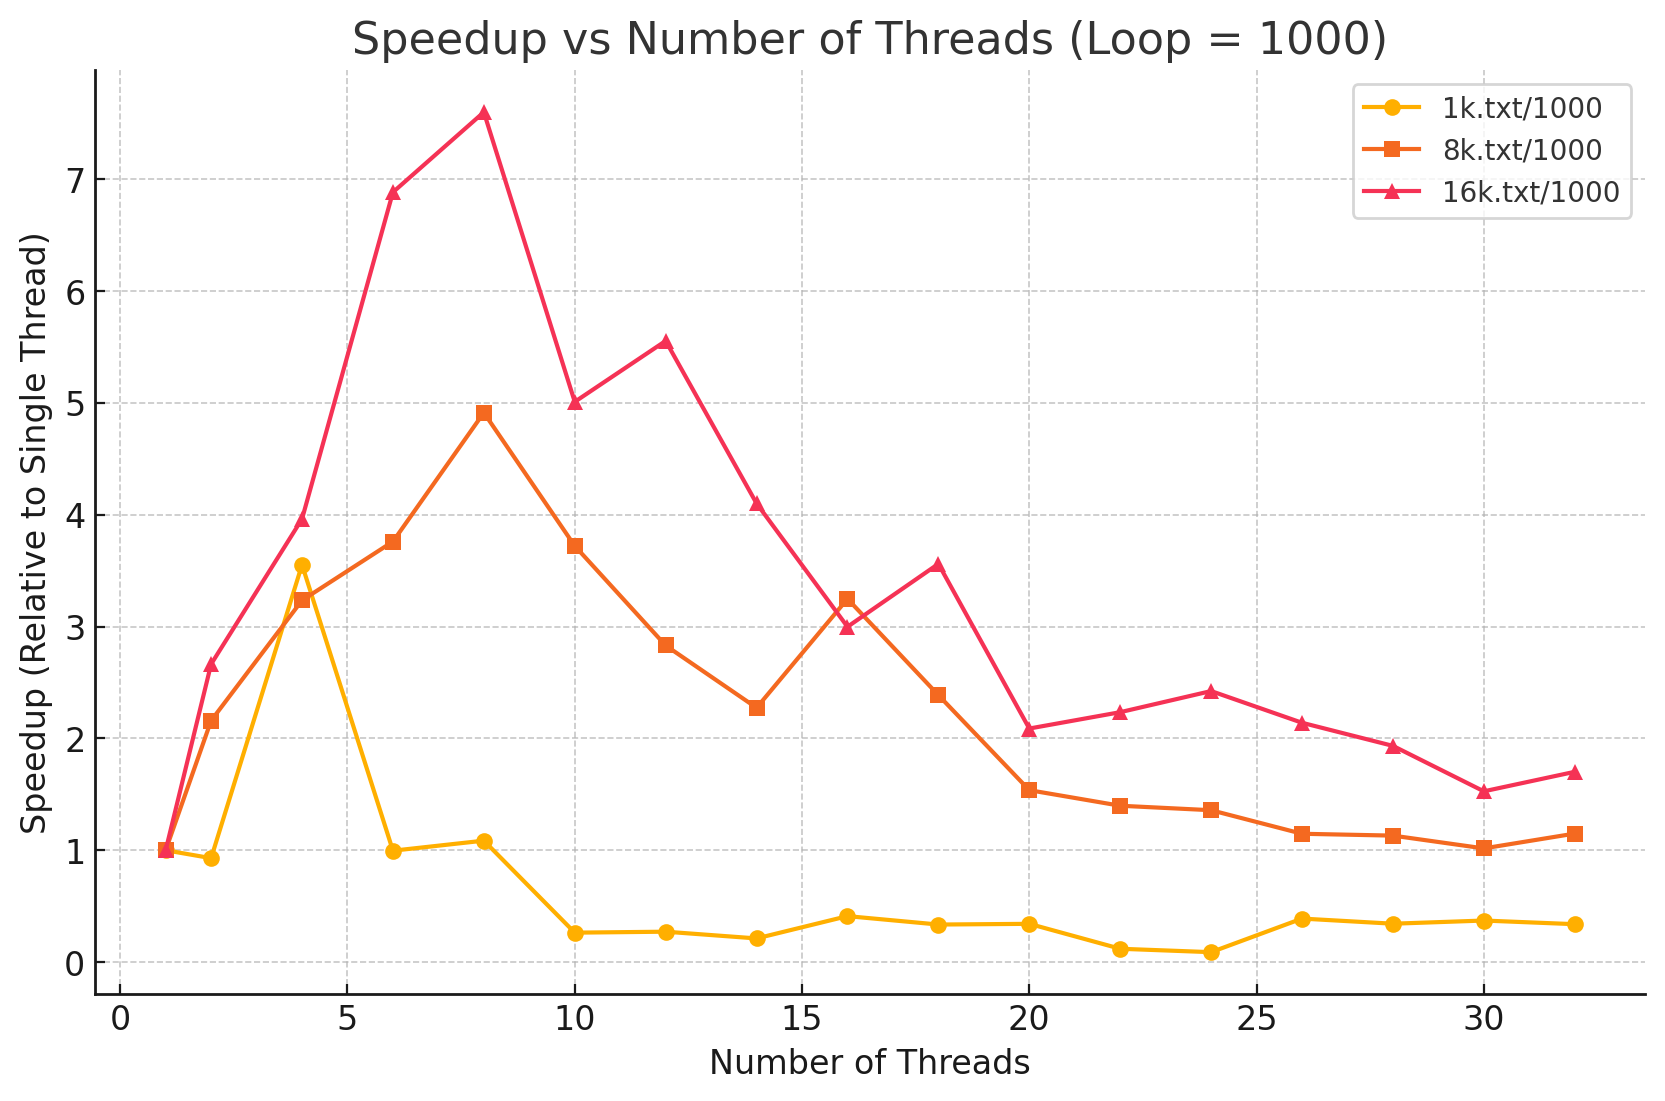
\includegraphics[width=\textwidth]{pthread_wait_speedup.png}
        \caption{Number of Threads VS. Speed-Up}
        \label{fig:ThreadVsSpeedUp1}
    \end{subfigure}
    \hfill  % Horizontal space between figures
    \begin{subfigure}[t]{0.48\textwidth}  % Adjusted width for side-by-side
        \centering
        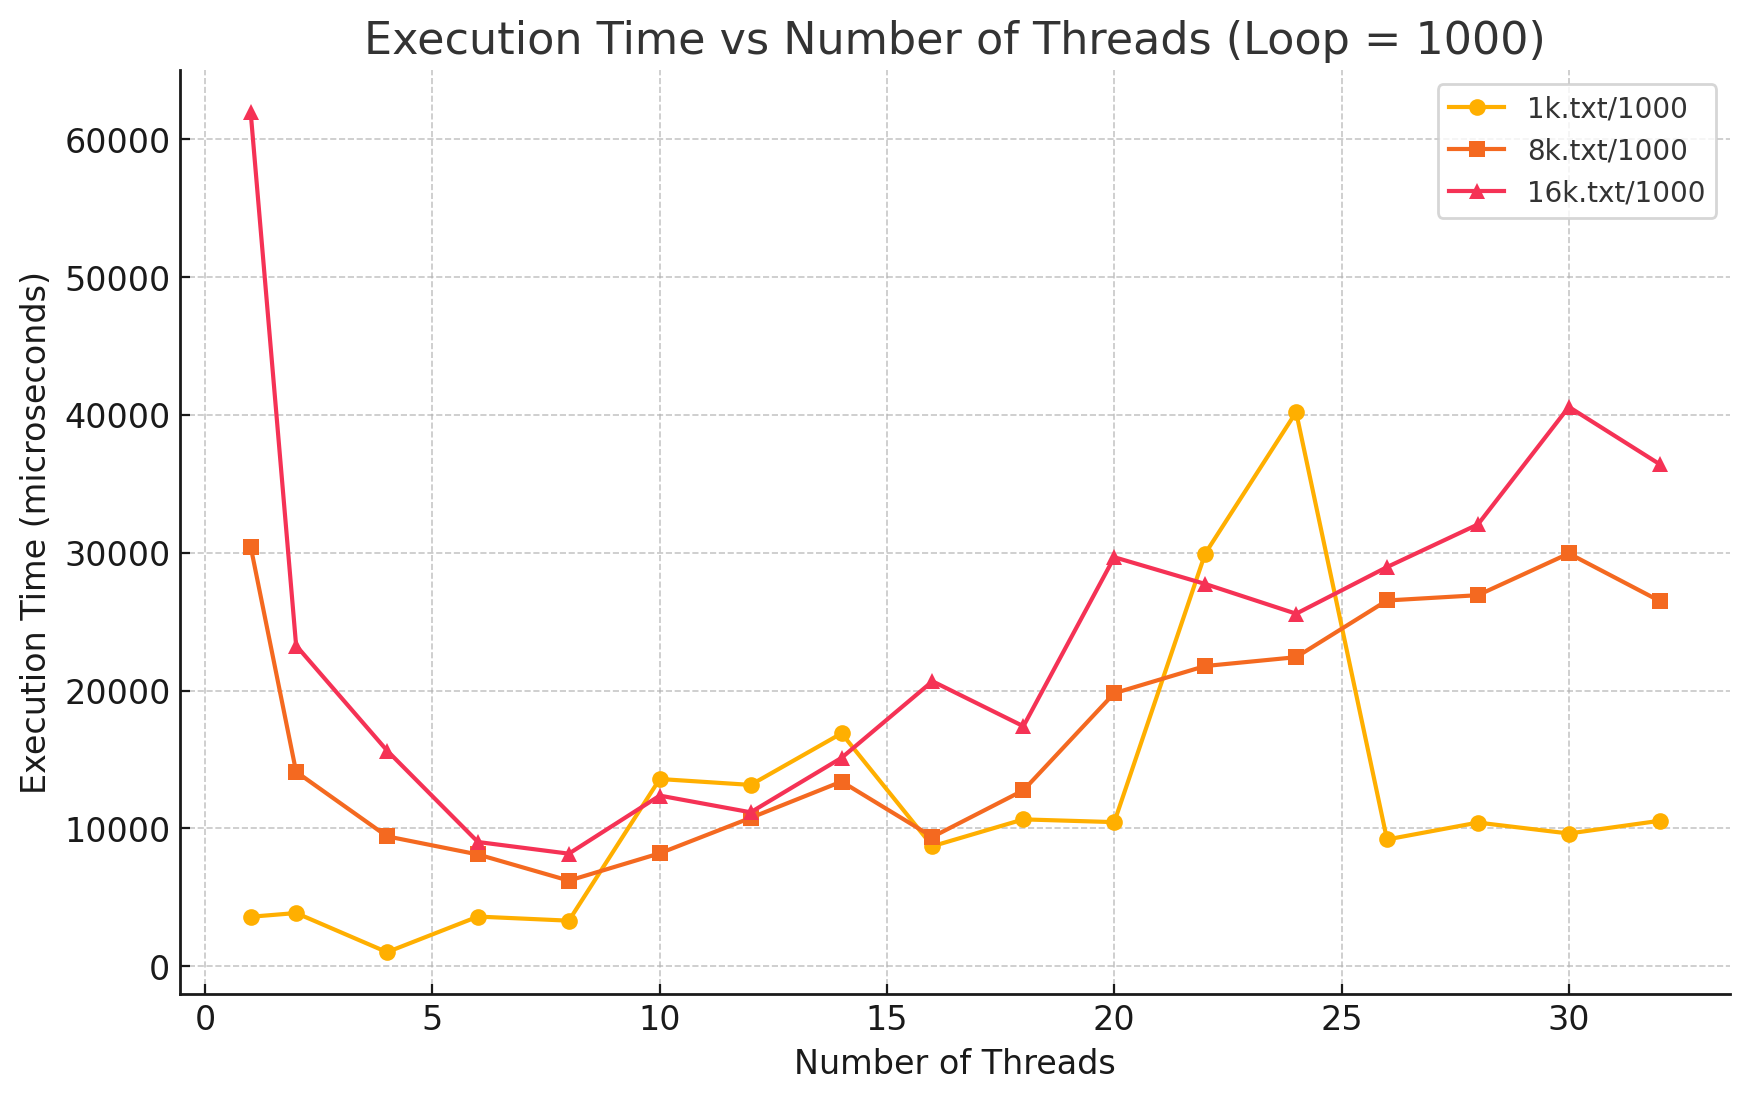
\includegraphics[width=\textwidth]{pthread_wait_execution.png}
        \caption{Number of Threads VS. Execution Time}
        \label{fig:ThreadVsExecutionTime}
    \end{subfigure}
    \caption{Speed-Up graph and Execution Time graph for loop = 1000}
    \label{fig:ThreadVsComparison}
\end{figure}
\hfill  % Horizontal space between figures



\section{Analysis and comparison}
Some improvements that I added in prefix\_sum function to help with performance  \\
1. Hybrid Approach for Small Inputs
\[
\text{if } n \leq 1024 \text{ and } n\_loops \leq 100:
\]
For small input sizes, the prefix sum is calculated sequentially, bypassing the overhead of thread creation and synchronization. This ensures better performance for small inputs where parallelization is not beneficial.\\

2. Static Work Distribution
Each thread is assigned a static range of the input array:
\[
\text{chunk\_size} = \frac{n + \text{num\_threads} - 1}{\text{num\_threads}}
\]
This ensures balanced work distribution across threads, reducing contention and avoiding overloading any single thread.\\

3. Reduced Synchronization Frequency
Synchronization barriers are applied every few iterations, rather than after each step:
\[
\text{if } d \% \text{sync\_interval} = 0 \text{, then barrier\_wait();}
\]
This reduces the overhead from frequent synchronization, allowing threads to work more independently.

4. Parallelized Up-Sweep and Down-Sweep Phases
The Blelloch algorithm is applied in parallel:
\[
\text{stride} = 2^{d+1} \quad (\text{up-sweep and down-sweep phases})
\]
This enables efficient parallelization of both phases, allowing threads to work on separate sections of the array, minimizing inter-thread dependencies.\\

5. Tunable Synchronization Interval
The synchronization interval can be adjusted for further optimization:
\[
\text{sync\_interval} = 2
\]
This allows fine-tuning of synchronization frequency to balance performance and correctness.\\

6. Efficient Identity Element Setting
Only the thread with \texttt{thread\_id = 0} sets the identity element in the output:
\[
\text{if } \text{thread\_id} = 0: \quad \text{output}[n-1] = 0
\]
This prevents redundant work and allows other threads to continue with the down-sweep phase.

\subsection{Performance}
\subsubsection{Performance with different input size}
s we can see from the graphs above, larger input sizes generally result in better performance. 
This is because larger workloads provide more opportunities to parallelize the computation across threads. 
With smaller inputs, the overhead of thread management and synchronization outweighs the benefits of parallel execution. For larger inputs, the results are more consistent, and we observe fewer drastic changes in speedup as we increase the number of threads. This consistency is due to the workload being large enough to keep all threads busy, 
which helps mitigate the relative impact of synchronization overhead.

\subsubsection{Performance with different loop size}
With loop size = 10, the speedup is not significant, we can observe speedup drops as we add more threads because the Synchronization Overhead dominate the performance and makes it not speeding up.

starting from loop size = 100, the speedup is much better when we add more threads to it, but at some point we will see a peak in performance, and after that adding more threads does not increase the overall speedup.
As we increase the loop size, the speedup vs threads result becomes more consistent and not increasing or decreasing too much, adding more threads at this phase doesn't add much value in terms of performance.


\subsubsection{Performance with Sleep VS. Yield}
I noticed that when we use sleep, the performance is somewhat consistent, adding more threads will help, but up to a point, then adding more threads does not improve too much.\\
However for yield, when we yield and slowly increase number of threads, the performance peaked at a certain number, then it began to be worse than the peak performance. \\
The reason might be with many threads (especially more threads than CPU cores), yielding threads can create a lot of context switching. Each yielded thread is still ready to be run, and the CPU needs to frequently switch between threads. This context-switching overhead increases with more threads, which degrades performance and leads to inefficient CPU utilization.\\
 Yielding can result in threads getting rescheduled frequently as well, this constant checks is wasting CPU resources because the system is repeatedly putting threads on and off.
 But with sleep, when a thread sleeps, it is removed from the ready queue for the duration of the sleep period. This reduces the number of context switches the OS needs to manage, as the sleeping threads are not immediately rescheduled. This gives the CPU more time to focus on threads that are actively doing useful work.
I did not go through the backoff strategies and test them out, but in terms of performance it should help as well.\\

\subsubsection{Performance with Codio VS. MacOS}
In my tests, I also observed performance differences between running the program on Codio and macOS. On Codio, which runs in a virtualized environment, speed up tends to be less. The overhead of running in a virtual machine can limit the system's ability to efficiently manage a large number of threads, resulting in lower overall speedup. However the results does look consistent especially with large input and higher loop size.
In contrast, running the program on macOS, which runs directly on the hardware, provides more consistent and predictable performance. Since there are no virtualization layers, macOS can fully utilize the system’s CPU and memory resources. This results in better thread management, fewer performance bottlenecks, and higher speedup, particularly when dealing with larger input sizes and more threads.
However, the performance differences also depend on the underlying hardware. macOS running on a multi-core system can take advantage of the available cores to parallelize workloads more efficiently, while a limited number of cores in the virtual environment on Codio may restrict the achievable performance improvements.


\subsection{Scalability}
The implementation of the parallel prefix sum function using the Blelloch algorithm and a spin barrier shows good scalability characteristics, particularly with larger input sizes and increased loop counts. Below is a summary of the key factors affecting scalability:

\subsubsection{Performance with Large Inputs}
For large inputs, the static work distribution and parallel nature of the Blelloch algorithm result in efficient load balancing across threads. Since the up-sweep and down-sweep phases scale logarithmically with the input size ($O(\log n)$), the performance improves significantly when more threads are used. In the tests conducted, it was observed that:

\[
\text{Larger inputs lead to better performance as the number of threads increases.}
\]

\subsubsection{ Synchronization Overhead}
The spin barrier, mitigates the overhead caused by synchronization. By reducing the synchronization frequency (every second iteration), the number of synchronization points is minimized. This reduces thread contention and improves performance, especially with larger inputs.

However, as the number of threads increases, synchronization overhead can still become a bottleneck. This is more apparent in smaller input sizes where the cost of synchronization is higher relative to the computational workload.

\subsubsection{Impact of Loop Count}
When the number of loops in the operation increases, the performance impact becomes more noticeable. Larger loop counts provide more opportunities for parallel computation to outweigh synchronization overhead. In the tests, increasing the loop count further improved scalability, particularly for larger input sizes.

\[
\text{Increasing the loop count amplifies the performance benefits for larger inputs.}
\]

\subsubsection{Limited Scalability with Small Inputs}
For small inputs, the overhead of thread creation and synchronization outweighs the benefits of parallelism. In such cases, the hybrid approach (where the computation is performed sequentially for small inputs) prevents the overhead of thread management. However, even with this optimization, the scalability for smaller inputs is limited.

\subsubsection*{Conclusion}
The implementation scales well for large inputs and high loop counts. Synchronization overhead, managed via the custom spin barrier, is minimized effectively but can still become a limiting factor with small inputs or an excessive number of threads. Based on the test results, it was found that:

\[
\text{Performance is significantly better for larger inputs, especially when the loop count is increased.}
\]

\subsection{Efficiency}
Efficiency is defined as the speedup divided by the number of threads. 
Figure bellow shows the efficiency of the implementation, which decreases as more threads are added due to increasing synchronization costs.

\begin{figure}[H]
    \centering
    \begin{subfigure}[t]{0.48\textwidth}  % Adjusted width for side-by-side
        \centering
        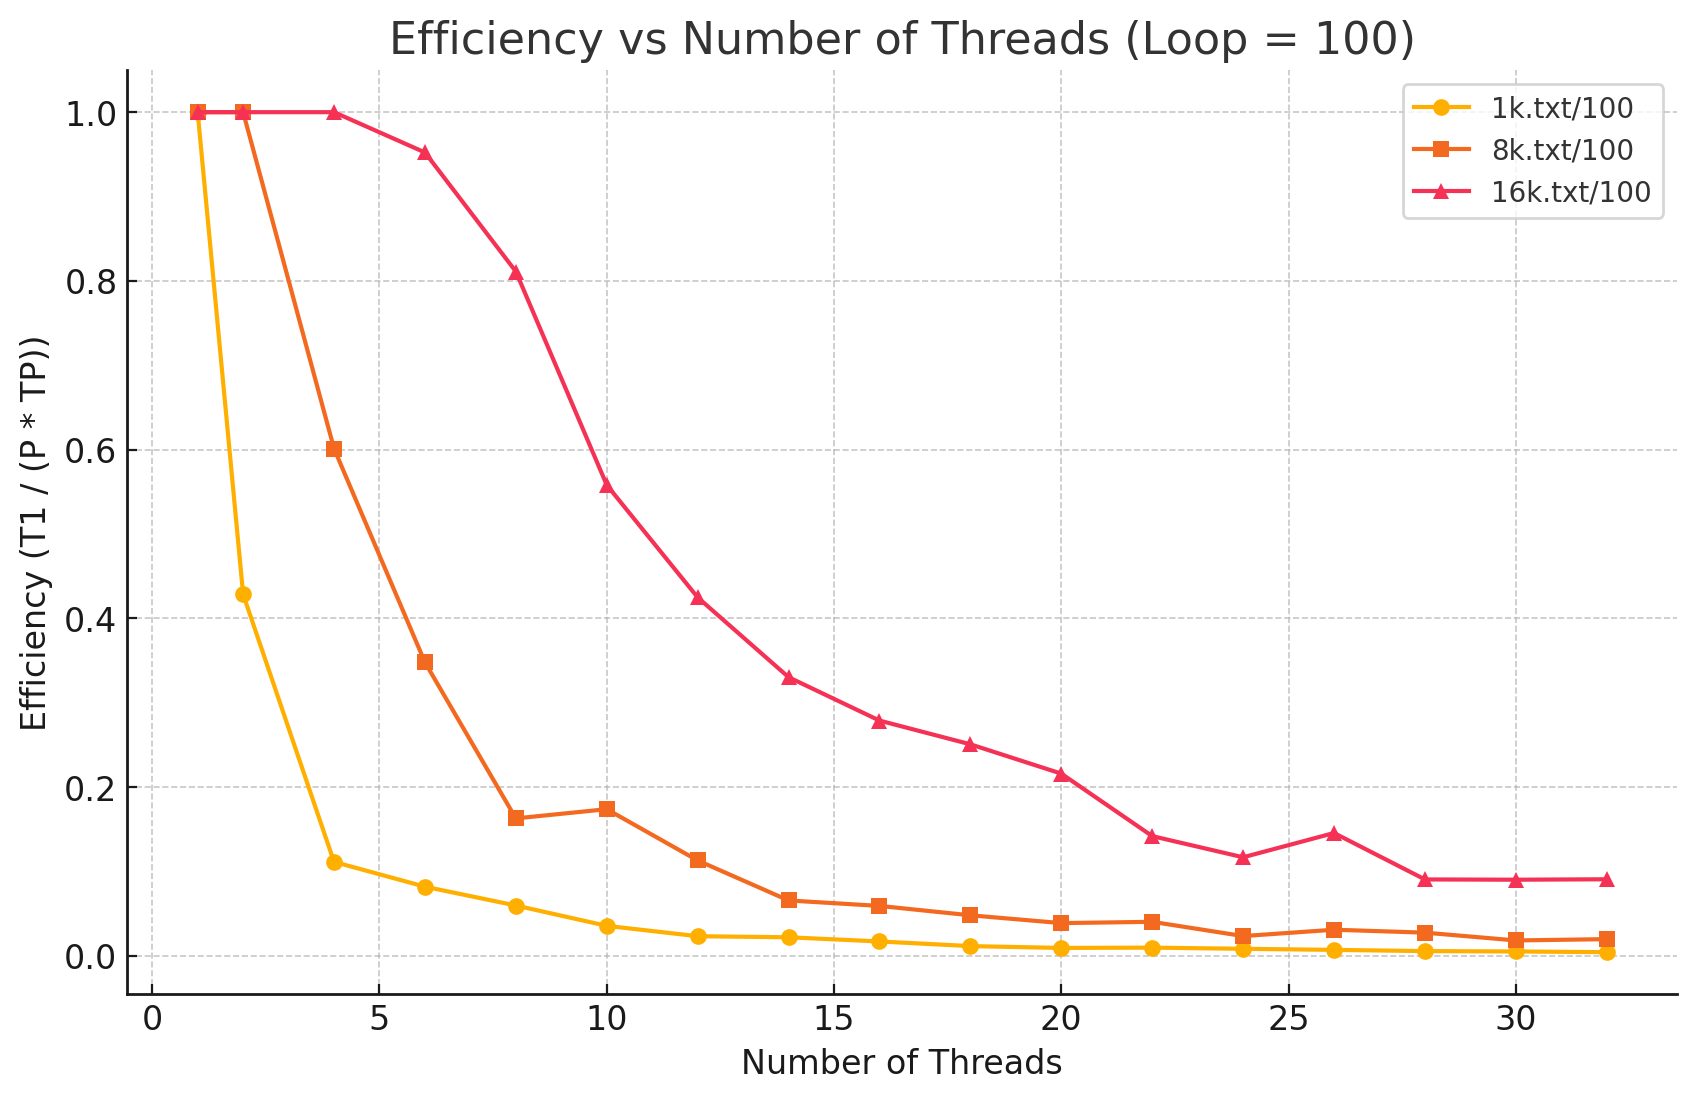
\includegraphics[width=\textwidth]{efficiency100.png}
        \caption{Number of Threads VS. Efficiency loop = 100}
        \label{fig:ThreadVsEfficiency}
    \end{subfigure}
    \hfill  % Horizontal space between figures
    \begin{subfigure}[t]{0.48\textwidth}  % Adjusted width for side-by-side
        \centering
        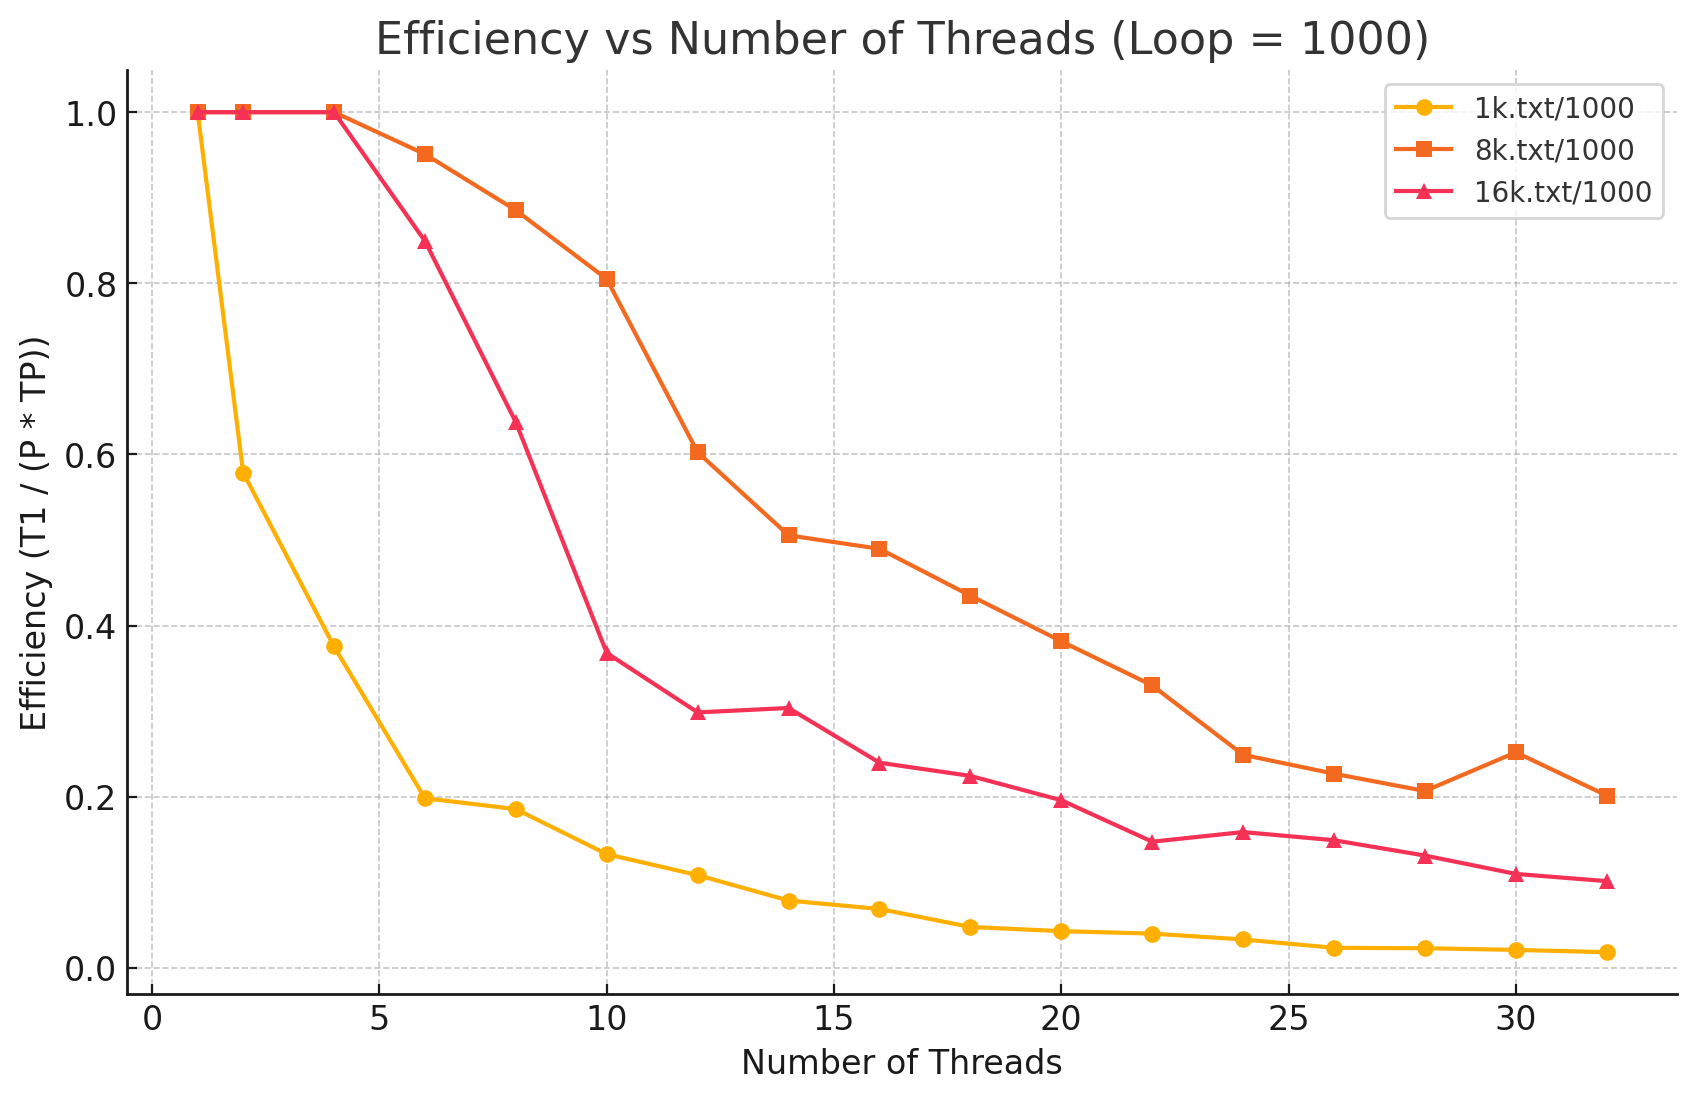
\includegraphics[width=\textwidth]{efficiencyloop1000.png}
        \caption{Number of Threads VS. Efficiency loop = 1000}
        \label{fig:ThreadVsEfficiency}
    \end{subfigure}

   \label{fig:ThreadVsEfficiency}
\end{figure}
\hfill  % Horizontal space between figures


\begin{figure}[H]
    \centering
    \begin{subfigure}[t]{0.48\textwidth}  % Adjusted width for side-by-side
        \centering
        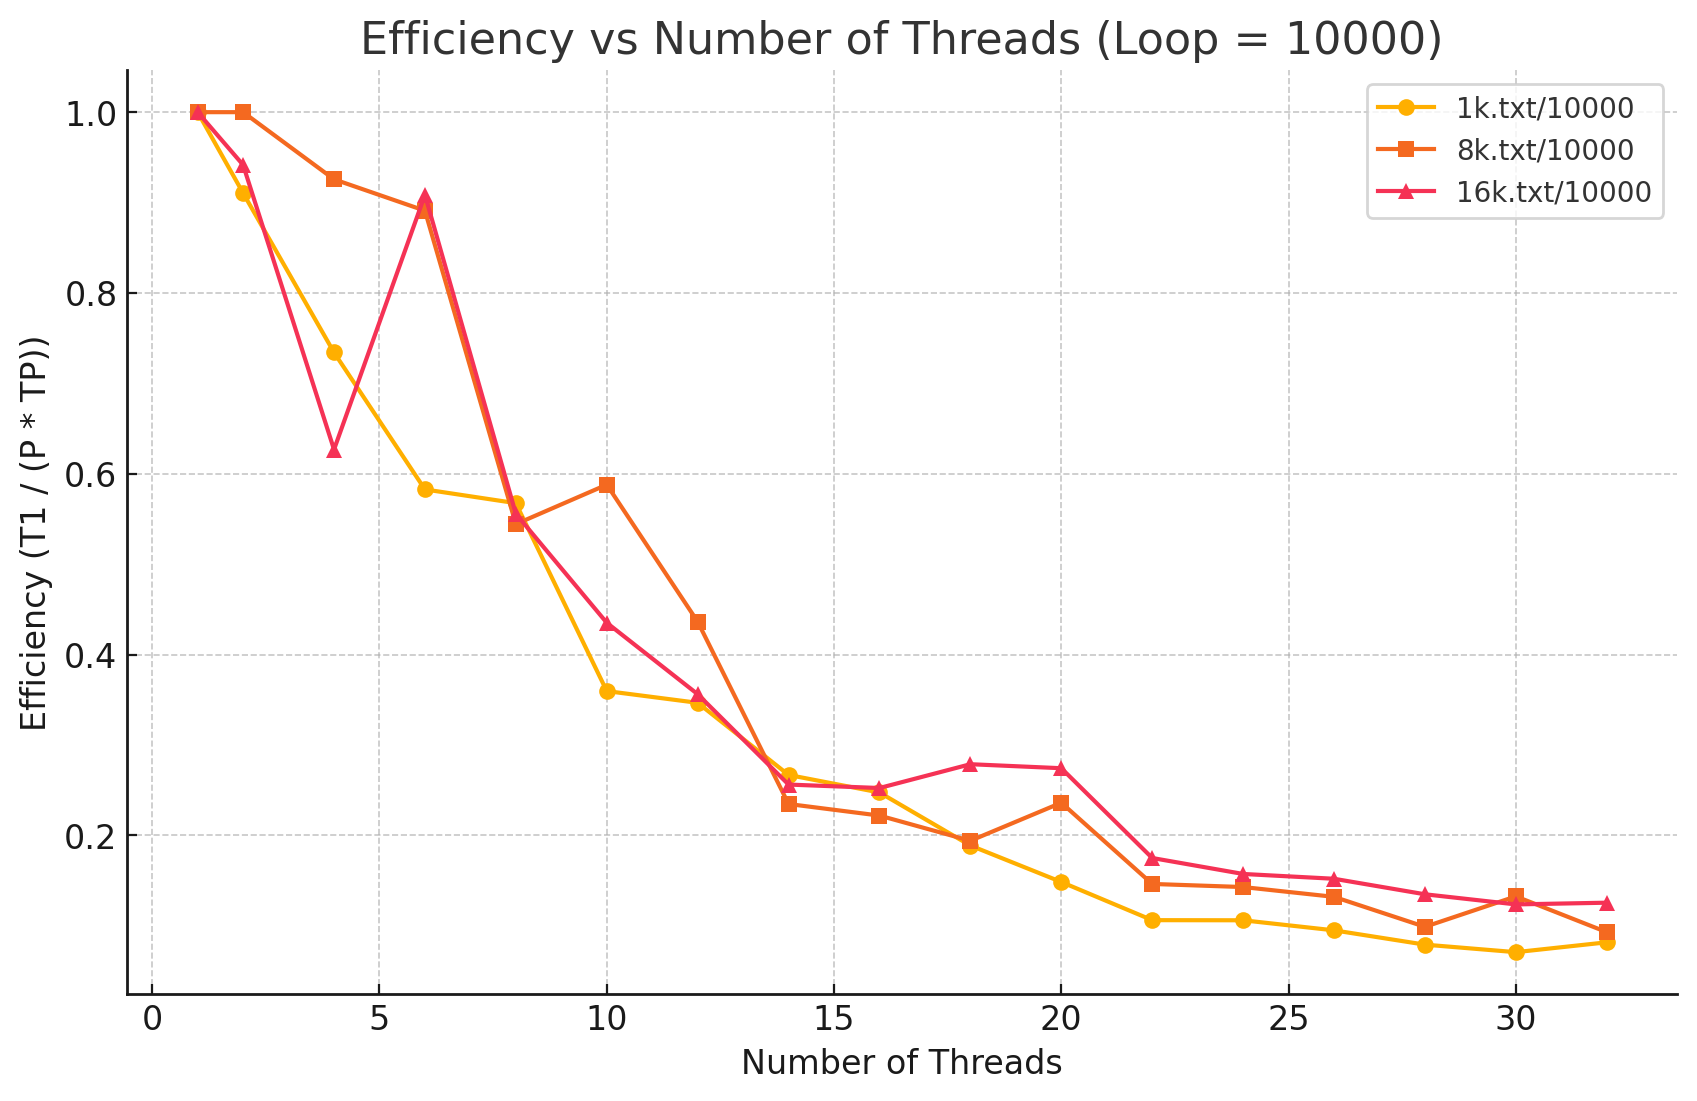
\includegraphics[width=\textwidth]{efficiency10000.png}
        \caption{Number of Threads VS. Efficiency loop = 10000}
        \label{fig:ThreadVsEfficiency}
    \end{subfigure}
    \hfill  % Horizontal space between figures
    \begin{subfigure}[t]{0.48\textwidth}  % Adjusted width for side-by-side
        \centering
        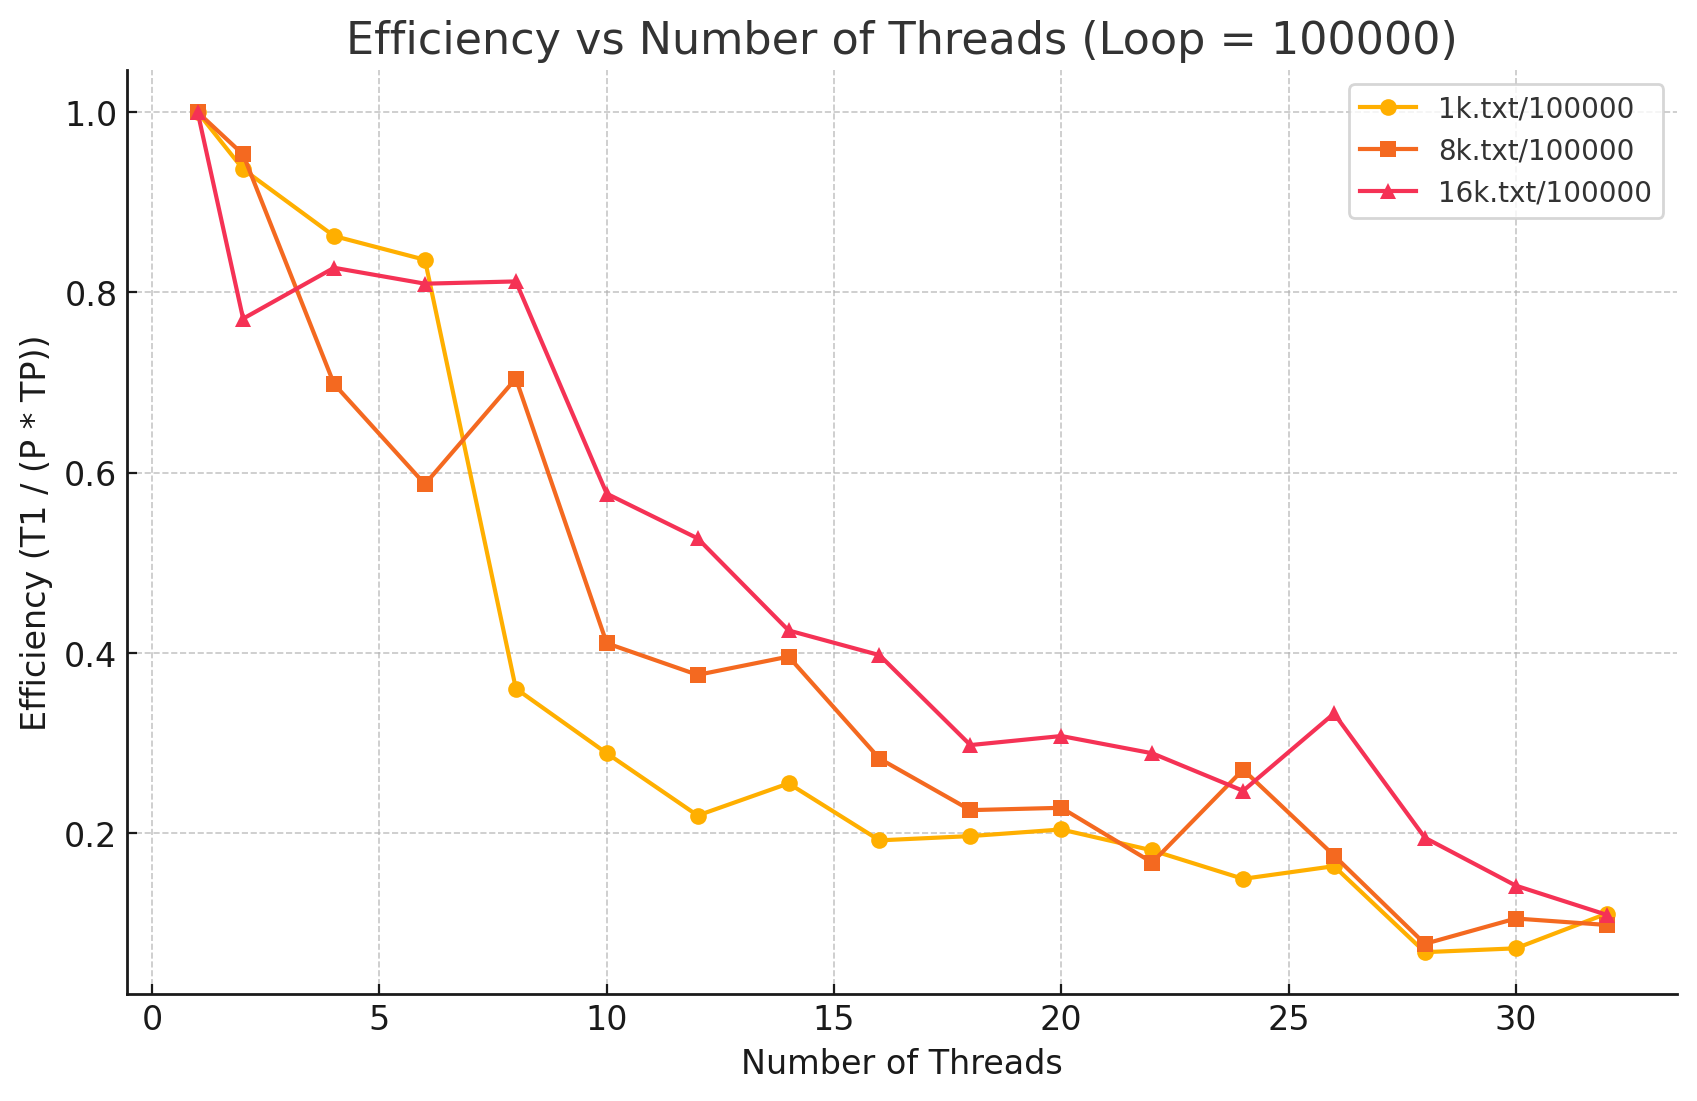
\includegraphics[width=\textwidth]{efficiency100000.png}
        \caption{Number of Threads VS. Efficiency loop = 100000}
        \label{fig:ThreadVsEfficiency}
    \end{subfigure}
   \label{fig:ThreadVsEfficiency}
\end{figure}
\hfill  % Horizontal space between figures



   $$E = \frac{S}{P} = \frac{\frac{T_1}{T_P}}{P} = \frac{T_1}{P \cdot T_P}$$

  

This formula expresses the proportion of the ideal performance achieved by the parallel program. The ideal efficiency is $100\%$, meaning that each thread is contributing fully to reducing the execution time.

The prefix sum implementation using the Blelloch algorithm and a spin barrier demonstrates several key aspects of efficiency. This section summarizes the efficiency factors observed from the tests conducted.

\subsubsection{Efficiency with different input sizes}
For large inputs, the workload is distributed evenly across threads, leading to better utilization of computational resources. The logarithmic depth of the Blelloch algorithm (\( O(\log n) \)) combined with parallelization allows the implementation to scale efficiently with thread count. However, while larger input sizes generally improve efficiency, the data shows that increasing the number of threads eventually leads to diminishing returns due to the overhead of managing and synchronizing threads.\\
Efficiency improves with larger inputs, but thread synchronization overhead becomes more prominent at higher thread counts.\\\\
For smaller inputs, the overhead from thread management and synchronization outweighs the computational benefits of parallelism. The implementation attempts to mitigate this inefficiency with a hybrid sequential approach, but even so, the overhead dominates the computational workload for small inputs, leading to lower efficiency.\\
Efficiency drops significantly with small inputs due to synchronization overhead dominating computation.

\subsubsection{Impact of Loop Count}
Increasing the loop count ideally should improve efficiency, particularly with larger inputs. As the workload per thread grows, the relative cost of synchronization decreases, allowing the system to achieve better CPU utilization. However, beyond a certain point, increasing the number of threads introduces significant overhead, even for higher loop counts, which limits the potential efficiency gains.\\
From test results, higher loop counts improve efficiency not by a lot, the overall efficiency still drops drastically comparing with smaller loop size, it drops even faster. It could be because of increased synchronization overhead as mroe threads are added. The cost of managing and synchronizing many threads eventually outweights the benefits., resource contention and thread management overhead becomes more significant.


\subsubsection{Scalability and Efficiency Trade-off}
While the implementation scales well up to a point, efficiency decreases as more threads are added due to the increasing cost of thread synchronization. This trade-off becomes especially noticeable with small inputs, where the synchronization overhead dominates the actual computation.
In conclusion:
Efficiency decreases beyond a certain thread count as synchronization overhead outweighs computational gains, particularly for small inputs.\\

\subsubsection{Conclusion}
The implementation achieves high efficiency with large inputs and high loop counts, particularly when the computational workload per thread is sufficient to mitigate the overhead of synchronization. However, as the number of threads increases beyond a certain threshold, synchronization overhead becomes more significant, especially with small inputs. Performance improves with more threads up to a point, but beyond that, synchronization costs, resource contention, and management overhead increase faster than the benefits of parallelism, leading to a performance bottleneck.

Small inputs and excessive threads introduce bottlenecks that limit efficiency, highlighting the importance of balancing workload and thread count to maximize performance.




 


\section*{Conclusions}

The experiments show that the Blelloch prefix sum algorithm performs efficiently for large input sizes. However, for smaller input sizes, the synchronization overhead limits the achievable speedup, and the CPU cores, memory bandwidth are also bottleneck of the current limited speedup we observe. Up to a point, adding threads no longer increase the speed-up due to multiple reasons.


  






\section*{6. References}


\subsection*{Technical Sources:}

\begin{itemize}

    \item \href{https://medium.com/nerd-for-tech/understanding-implementation-of-work-efficient-parallel-prefix-scan-cca2d5335c9b}{Understanding Implementation of Work-Efficient Parallel Prefix Scan}
    \item \href{https://www.cs.utexas.edu/~rossbach/cs380p/lab/prefix-sum-pthreads-cs380p.html}{Lab 1: Prefix Scan and Barriers}
    \item \href{https://www.cs.cmu.edu/~guyb/papers/Ble93.pdf}{Guy E. Blelloch: Prefix Sums and Their Applications}
    \item \href{https://www.cs.utexas.edu/~rossbach/cs380p/lectures/06-Conditions+Barriers.pdf}{CS380P Lecture: Conditions and Barriers}
    \item \href{https://en.cppreference.com/w/cpp/atomic/memory_order}{C++ Atomic Memory Order Reference}
    \item \href{https://medium.com/@joao_vaz/spin-lock-in-modern-c-with-atomics-memory-barriers-and-exponential-back-off-522798aca817}{Spin-Lock in Modern C++ with Atomics, Memory Barriers, and Exponential Back-Off}
    \item \href{https://coffeebeforearch.github.io/2020/11/07/spinlocks-6.html}{Spinlocks in C++ with CoffeeBeforeArch}
    \item \href{https://developer.nvidia.com/gpugems/gpugems3/part-vi-gpu-computing/chapter-39-parallel-prefix-sum-scan-cuda}{Chapter 39. Parallel Prefix Sum (Scan) with CUDA}
   \end{itemize}

\end{document}
